\documentclass[a4paper,12pt]{scrbook}

\usepackage{latexki}
\lecturer{Prof. Dr. F. Herrlich}
\semester{Sommersemester 2006}
\scriptstate{complete}


% Deutsche Sprache
\usepackage{ngerman}

% Verschiebt \sections auf die naechste seite falls sie zu tief sind. Muss vor
% hyperref kommen.
\usepackage[nobottomtitles]{titlesec}

% Schicke Schrift
\usepackage[utf8]{inputenc}
\usepackage[T1]{fontenc}
\usepackage{lmodern}

% schmaler rand
\usepackage{geometry}
\geometry{a4paper,tmargin=2cm,lmargin=2cm,rmargin=2cm}

\setlength\parskip{\smallskipamount}
\setlength\parindent{0pt}
\tolerance=900

% Vokabelliste erzeugen
\usepackage{index}
\newindex{default}{idx}{ind}{Vokabeln}

% links
\usepackage{color}
\usepackage{hyperref}

\definecolor{rltred}{rgb}{0.75,0,0}
\definecolor{rltgreen}{rgb}{0,0.5,0}
\definecolor{rltblue}{rgb}{0,0,0.75}

\hypersetup{
  pdftitle={Algebra II Prof. Herrlich},
  pdfsubject={Algebra II},
  pdfkeywords={Algebra II Herrlich A2},
  pdfproducer={pdfLaTeX},
  pdfpagemode={UseOutlines},
  colorlinks=true,
  bookmarksopen=true,
  bookmarksnumbered=true,
  urlcolor=rltblue,
  filecolor=rltgreen,
  linkcolor=rltblue,
  backref=true,
  pagebackref=true,
  pdfpagemode=None
}

% Mathe-Pakete
\usepackage{amssymb}
\usepackage{amsmath}
\usepackage{amsfonts}
\usepackage{stmaryrd}

% Für Diagramme
\usepackage[arrow,matrix,curve]{xy}

\usepackage{etex}
\usepackage{pictex}
\usepackage{graphicx}

% Theorem-Umgebung
\usepackage[hyperref,amsmath,thmmarks,thref]{ntheorem}

% keine kursiv schrift in theorems
\theorembodyfont{}

% Theoreme definieren
\theoremstyle{break}
    \newtheorem{Satz}{Satz}
    \newtheorem{SatzDef}[Satz]{Satz + Definition}
    \newtheorem{Def}{Definition}[chapter]
    \newtheorem{DefBem}[Def]{Definition + Bemerkung}
    \newtheorem{Bem}[Def]{Bemerkung}
    \newtheorem{BemDef}[Def]{Bemerkung + Definition}
    \newtheorem{Prop}[Def]{Proposition}
    \newtheorem{PropDef}[Def]{Proposition + Definition}
    \newtheorem{Folg}[Def]{Folgerung}
    \newtheorem{Bsp}[Def]{Beispiele}
    \newtheorem{DefProp}[Def]{Definition + Proposition}
    \newtheorem{anBew}[Def]{Beweis}
\theoremstyle{nonumberbreak}
    \newtheorem{Bew}{Beweis}
    \newtheorem{nnBem}{Bemerkung}
    \newtheorem{nnBsp}{Beispiele}
    \newtheorem{nnSatz}{Satz}
    \newtheorem{nnFolg}{Folgerung}
    \newtheorem{Beo}{Beobachtung}
    \newtheorem{Eri}{Erinnerung}
\theoremstyle{nonumberplain}
    \theoremsymbol{\ensuremath{\Box}}
    \newtheorem{proof}{Beweis}

\newcommand{\emp}[1]{\textbf{\emph{#1}}}
\newcommand{\defeqr}[0]{\mathrel{\mathop:}=}
\newcommand{\defeql}[0]{=\mathrel{\mathop:}}

\newcommand{\myref}[2]{%
\hyperref[#2]{#1~\ref*{#2}}%
}

\DeclareMathOperator{\Aut}{Aut}
\DeclareMathOperator{\Hom}{Hom}
\DeclareMathOperator{\Quot}{Quot}

\DeclareMathOperator{\Kern}{Kern}
\DeclareMathOperator{\Bild}{Bild}

\newcommand{\FakRaum}[2]{
  \raisebox{0.7ex}{\ensuremath{#1}}
  \ensuremath{\mkern-3mu}\big/\ensuremath{\mkern-3mu}
  \raisebox{-0.6ex}{\ensuremath{#2}}} 

\renewcommand{\labelenumi}{\theenumi}    
\renewcommand{\theenumi}{(\alph{enumi})}

\renewcommand{\OE}{O\!\!E}

% Weniger Abstand nach der Ueberschrift des Inhaltsverzeichnises
\makeatletter
\let\@my@starttoc\@starttoc
\renewcommand*{\@starttoc}[1]{%
  \addvspace{-1.5em}%
  \@my@starttoc{#1}%
}
\makeatother

% Einige Anstrengungen, um den § vor die Section-Nummer zu stellen
% \renewcommand{\thesection} allein führt zu einem Konflikt mit ntheorem-hyper
\makeatletter
\def\@seccntformat#1{\@ifundefined{#1@cntformat}%
{\csname the#1\endcsname\quad}% default
{\csname #1@cntformat\endcsname}% individual control
}
\def\section@cntformat{§\@arabic\c@section\quad}
\makeatother

\title{Algebra II}
\subtitle{Sommersemester 2006\\ Prof. Dr. F. Herrlich}
\author{Die Mitarbeiter von \url{http://lkwiki.nomeata.de/}}

\begin{document}
\maketitle

% Inhaltsverzeichnis
\pdfbookmark[1]{Inhaltsverzeichnis}{contents}
\setlength\parskip{0.6pt}
\tableofcontents

% Liste der benannten Saetze
\section*{Benannte Sätze}
\pdfbookmark[1]{Benannte Sätze}{contents}

\theoremlisttype{optname}
\listtheorems{Satz,SatzDef,Def,DefBem,BemDef,Prop,PropDef,Bsp,DefProp}

\setlength\parskip{\smallskipamount}


\chapter{Multilineare Algebra}

\section{Moduln}

Sei $R$ ein (kommutativer) Ring (mit Eins) (in der ganzen Vorlesung).

\begin{Def}
\label{1.1}
  \begin{enumerate}
    \item Eine abelsche Gruppe $(M,+)$ zusammen mit einer Abbildung
          $\cdot : R \times M \to M$ heißt \emp{$R$-Modul}\index{R-Modul} (genauer:
          $R$-Linksmodul), wenn gilt:
          \begin{enumerate}
            \item[(i)] $a \cdot (x+y) = a \cdot x + a \cdot y$
            \item[(ii)] $(a+b) \cdot x = a \cdot x + b \cdot x$
            \item[(iii)] $(a \cdot b) \cdot x = a \cdot (b \cdot x)$
            \item[(iv)] $1 \cdot x = x$
          \end{enumerate}
          für alle $a,b \in R,\;x,y \in M$.
    \item Eine Abbildung $\varphi: M \to M'$ zwischen $R$-Modulen $M$, $M'$
          heißt \emp{$R$-Modul-Homo\-morphismus}\index{R-Modul!-Homomorphismus} (kurz
          \emp{$R$-linear}\index{R-linear}), wenn für alle $x,y \in M, \; a,b \in R$
          gilt:\\
          $\varphi (a \cdot x + b \cdot y) = a \cdot \varphi (x) + b \cdot
          \varphi (y)$
  \end{enumerate}
\end{Def}

\begin{nnBsp}
  \begin{enumerate}
    \item[(1)] $R = K$ Körper. Dann ist $R$-Modul = $K$-Vektorraum und
               $R$-linear = linear
    \item[(2)] $R$ ist $R$-Modul. Jedes Ideal $I \subseteq R$ ist $R$-Modul
    \item[(3)] Jede abelsche Gruppe ist ein $\mathbb{Z}$-Modul.\\
               (denn: $n \cdot x = \underbrace{x + x + \cdots + x}_{n\text{-mal}}$
               definiert die Abbildung $\cdot: \mathbb{Z} \times M \to M$
               wie in \ref{1.1} gefordert)
  \end{enumerate}
\end{nnBsp}

\begin{BemDef}
  \begin{enumerate}
    \item Sind $M,M'$ $R$-Moduln, so ist Hom$_R(M,M') = \{\varphi: M \to M' :
          \varphi \text{ ist } R\text{-linear}\}$ ein $R$-Modul durch
          $(\varphi_1 + \varphi_2)(x) = \varphi_1(x) + \varphi_2(x)$ und
          $(a \cdot \varphi_1)(x) = a \cdot \varphi_1(x)$.
    \item $M^* = \Hom_R(M,R)$ heißt dualer Modul.\index{R-Modul!dualer}
  \end{enumerate}
\end{BemDef}

% fuer das grosse kartesische produkt im naechsten absatz
\newcommand{\BIGOP}[1]{\mathop{\mathchoice%
{\raise-0.22em\hbox{\huge $#1$}}%
{\raise-0.05em\hbox{\Large $#1$}}{\hbox{\large $#1$}}{#1}}}
\newcommand{\bigtimes}{\BIGOP{\times}} 

\begin{nnBsp}
  $R = \mathbb{Z}$\\
  Hom$_R(\mathbb{Z}/2\mathbb{Z}, \mathbb{Z}) = \{ 0 \}$, denn $0 = \varphi(0) =
  \varphi(1 + 1) = \varphi(1)+\varphi(1) \Rightarrow \varphi(1) = 0$
\end{nnBsp}

\begin{Bem}[Ähnlichkeiten von Moduln mit Vektorräumen]
  Die $R$-Moduln bilden eine \emp{abelsche Kategorie}\index{Kategorie!abelsche} \emp{$R$-Mod}\index{Kategorie!R-Mod}.
  \begin{enumerate}
    \item Eine Untergruppe $N$ eines $R$-Moduls $M$ heißt $R$-Untermodul von
          $M$, falls $R \cdot N \subseteq N$.
    \item Kern und Bild $R$-linearer Abbildungen sind $R$-Moduln.
    \item Zu jedem Untermodul $N \subseteq M$ gibt es einen Faktormodul $M/N$.
    \item Homomorphiesatz:\\
      Für einen surjektiven Homomorphismus $\varphi: M \rightarrow N$ gilt:
      $M/\Kern(\varphi) \cong N$.
    \item \emph{Direktes Produkt}: Sei ${\{M_{i}\}}_{i \in I}$ eine beliebige
          Menge von Moduln. Dann ist ihr direktes Produkt
     	  $\Pi_i M_i = \bigtimes_i M_i$ gegeben durch die Menge aller Tupel ${(m_i)}_{i
     	  \in I}$ mit $m_i \in M_i$ und die $R$-Aktion ${r(m_i)}_{i \in I} = {(rm_i)}_{i \in I}$.

	  \emph{Direkte Summe}: Das gleiche wie beim direkten Produkt, jedoch dürfen in den 
	  Tupeln nur endlich viele $m_i \neq 0$ sein.
  \end{enumerate}
\end{Bem}

\begin{Bew}
  \begin{enumerate}
    \stepcounter{enumi}
    \item $\Kern(\varphi)$: Sei $\varphi: M \rightarrow N$ lineare Abbildung. $m \in \Kern(\varphi)$, $r \in R$:\\
          $\varphi(rm) = r\varphi(m) = 0 \Rightarrow R \cdot \Kern(\varphi) \subseteq \Kern(\varphi)$; Untergruppe klar

	  $\Bild(\varphi)$: $n \in \Bild(\varphi) $, d. h. $\exists\, m: n = \varphi
   	  (m), m \in M \Rightarrow r \in R:
	  rn = r \varphi(m) = \varphi(rm) \in \Bild(\varphi)  \Rightarrow R
	  \cdot \Bild(\varphi) \subseteq \Bild(\varphi)$
    \item $M$ abelsch $\Rightarrow$ jedes $N$ Normalteiler $\Rightarrow M/N$ ist
          abelsche Gruppe.

    	  Wir definieren $R$-Aktion auf $M/N$ durch $r(m + N) = rm + N$. Das ist 
    	  wohldefiniert, denn\\
	  $r((m+n)+N)=r(m+n) + N= rm + \underbrace{rn}_{\in N} + N = rm + N$

	  $r((m+N) + (m' + N ) ) = r((m+m')+N) = r(m+m') + N = rm + N + rm' + N =
	  r(m+N) + r(m'+N)$\\
	  Die restlichen drei Eigenschaften gehen ähnlich.
	  
    \item
	$$\begin{xy}
              \xymatrix{
                M \ar[rr]^{\varphi} \ar[rd] &     &  N \\
                                            &  M/\Kern(\varphi) \ar@{-->}[ur]_{\exists!\, \tilde{\varphi}}  & }
          \end{xy}$$
	  Wohldefiniertheit von $\tilde{\varphi}$:\\
	  Sei $k \in \Kern(\varphi): \varphi(m+k) = \varphi(m)$

	  surjektiv: $\forall n \in N: n = \varphi(m) = \tilde{\varphi}(m + \Kern(\varphi))$

	  injektiv: $m, m' \in M$ mit $\varphi(m) = \varphi(m') = n \in N \Leftrightarrow 
	  \varphi(m-m') = 0 \Rightarrow m + \Kern(\varphi)(m) = \Kern(\varphi)(m')$

	  $\tilde{\varphi}$ ist $R$-linear: Klar, wegen $\varphi$ $R$-linear.
  \end{enumerate}
\end{Bew}

\begin{Bem}
  \begin{enumerate}
    \item Zu jeder Teilmenge $X \subseteq M$ eines $R$-Moduls $M$ gibt es den von
          $X$ erzeugten Untermodul $$\langle X \rangle = \displaystyle 
          \bigcap_{\substack{M' \subseteq M\; \text{ Untermodul} \\ X \subseteq M'}} M' = \left\{
          \sum_{i=1}^n a_i x_i: n \in \mathbb{N}, a_i \in R, x_i \in X \right\}$$
    \item $B \subset M$ heißt \emp{linear unabhängig}\index{linear unabhängig},
          wenn aus $\displaystyle \sum_{i=1}^n \alpha_i b_i = 0$ mit $n \in
          \mathbb{N}, b_i \in B, \alpha_i \in R$ folgt $\alpha_i = 0$ für alle
          $i$.
    \item Ein linear unabhängiges Erzeugendensystem heißt
          \emp{Basis}\index{Basis}.
    \item Nicht jedes $R$-Modul besitzt eine Basis.

          Beispiel: $\mathbb{Z}/2\mathbb{Z}$ als $\mathbb{Z}$-Modul: $\{\bar{1}\}$
          ist nicht linear unabhängig, da $\underbrace{42}_{\not= 0 \text{ in } \mathbb{Z}} \cdot 1 = 0$
    \item Ein $R$-Modul heißt \emp{frei}\index{R-Modul!freier}, wenn er eine
          Basis besitzt.
    \item Ein freier $R$-Modul $M$ hat die Universelle Abbildungseigenschaft eines Vektorraums. Ist $B$ eine
          Basis von $M$, $f: B \to M'$ eine Abbildung in einen $R$-Modul M', so
          gibt es genau eine $R$-lineare Abbildung $\varphi: M \to M'$ mit
          $\varphi|_B = f$.
    \item Sei $M$ freier, endlich erzeugter Modul. Dann ist $M^*$ wieder frei und hat dieselbe
          Dimension wie $M$.
  \end{enumerate}
\end{Bem}

\begin{Bew}
  \begin{enumerate}
    \item[(f)] Sei $\{y_i\}_{i \in I}$ Familie von Elementen von $M'$.\\
      Sei $x \in M$. Durch $x=\sum_{i}a_ix_i$ ist $\{a_i\}_{i  \in I}$
      eindeutig bestimmt.\\
      Wir setzen: $\varphi(x):=\sum_i a_iy_i=\sum_ia_i\varphi(x_i)$

      \textbf{Beh. 1:} Falls $\{y_i\}_{i\in I}\;(y_i \neq y_j \text{ für } i\neq
      j)$ Basis von $M'$ ist, dann ist $\varphi$ ein Isomorphismus.\\
      \textbf{Bew. 1:} Wir können den Beweis des Satzes rückwärts anwenden\\
      $\Rightarrow$ $\exists\, \psi: M' \rightarrow M \text{ mit } \psi(y_i)=x_i \forall i \in I$\\
      $\Rightarrow$ $\varphi \circ \psi = id_N, \psi \circ \varphi = id_M$

      \textbf{Beh. 2:} Zwei freie Moduln mit gleicher Basis sind isomorph.\\
      \textbf{Bew. 2:} klar
  \end{enumerate}
\end{Bew}

\begin{PropDef}
  Sei $0 \to M' \overset{\alpha}{\to} M \overset{\beta}{\to} M'' \to 0$ kurze exakte Sequenz von $R$-Moduln (d.h.
  $M' \subseteq M$ Untermodul, $M'' = M/M'$). Dann gilt für jeden $R$-Modul $N$:
  \begin{enumerate}
    \item $0 \to \Hom_R(N,M') \overset{\alpha_*}{\to} \Hom_R(N,M) \overset{\beta_*}{\to}
          \Hom_R(N,M'')$ ist exakt.
    \item $0 \to \Hom_R(M'',N) \overset{\beta^*}{\to} \Hom_R(M,N) \overset{\alpha^*}{\to}
          \Hom_R(M',N)$ ist exakt.
    \item Im Allgemeinen sind $\beta_*$ bzw. $\alpha^*$ nicht surjektiv.
    \item Ein Modul $N$ heißt \emp{projektiv}\index{R-Modul!projektiver} (bzw.
          \emp{injektiv}\index{R-Modul!injektiver}), wenn $\beta_*$ (bzw.
          $\alpha^*$) surjektiv ist.
    \item Freie Moduln sind projektiv.
    \item Jeder $R$-Modul M ist Faktormodul eines projektiven $R$-Moduls.
    \item Jeder $R$-Modul M ist Untermodul eines injektiven $R$-Moduls.
  \end{enumerate}
\end{PropDef}

\begin{Bew}
  \begin{enumerate}
  \item $$
    \begin{xy}
      \xymatrix{
        &                    &  N \ar[ld]_\varphi \ar[d]^\psi \ar[dr] & & \\
	0 \ar[r] & M' \ar[r]^{\alpha} & M \ar[r]^{\beta} & M'' \ar[r] & 0
      }
    \end{xy}
    $$

    $\alpha_*$ ist injektiv: Sei $\varphi \in \Hom_R(N,M')$, ist
    $\alpha_*(\varphi) = \alpha \circ \varphi = 0 \overset{\alpha \text{ inj.}}{\Rightarrow} \varphi = 0$.

    $\Bild(\alpha_*) \subseteq \Kern(\beta_*)$:
    $\beta_*(\alpha_*(\varphi)) = \underset{=0}{\underbrace{\beta \circ \alpha}} \circ \varphi = 0$

    $\Kern(\beta_*) \subseteq \Bild(\alpha_*)$:\\
    Sei $\beta \circ \psi = 0$ ($\psi \in \Kern(\beta_*)$). Für jedes $x \in N$ ist $\psi(x) \in
    \Kern(\beta) = \Bild(\alpha) \Rightarrow$ zu $x \in N \;
    \exists\, y \in M' \text{ mit } \psi(x) = \alpha(y)$; $y$ ist
    eindeutig, da $\alpha$ injektiv.
    
    Definiere $\varphi': N \to M'$ durch $x \mapsto y$.\\
    Zu zeigen: $\varphi'$ ist $R$-linear\\
    Seien $x,x' \in N \Rightarrow \varphi'(x+x')=z$ mit $\alpha(z) =
    \varphi(x+x') = \varphi(x) + \varphi(x') = \alpha(y) + \alpha(y') =
    \alpha(y +y')$ mit $\varphi'(x) = y, \; \varphi'(x') = y'
    \overset{\alpha \text{ inj.}}{\Rightarrow} z = y + y'$

    Genauso: $\varphi'(a \cdot x) = a \cdot \varphi'(x)$
  \item \[
    \begin{xy}
      \xymatrix{
        0 \ar[r] & M' \ar[r] & M \ar[rr]^{\beta} \ar[rd]_{\beta^*(\varphi)} &  &  M'' \ar[dl]^{\varphi} \ar[r] & 0 \\
        & & & N & }
    \end{xy}
    \]
    $\beta^*$ injektiv, denn für $\varphi \in \Hom(M'', N)$ ist
    $\beta^*(\varphi)=\varphi\circ \beta$\\
    Sei $\beta^*(\varphi)= 0 \Rightarrow \varphi \circ \beta = 0 \overset{\beta
      \text{ surj.}}{\Rightarrow}\varphi=0$.

    $\Bild(\beta^*) \subseteq \Kern(\alpha^*)$: $(\alpha^* \circ 
    \beta^*)(\varphi)= \alpha^*(\varphi\circ \beta)=\varphi \circ
    \underbrace{\beta \circ \alpha}_{=0}=0$

    $\Kern(\alpha^*)\subseteq\Bild(\beta^*)$: Sei $\psi \in \Kern(\alpha^*)$.
    Aber $\psi \in \Hom_R(M, N)$ mit $\psi \circ \alpha=0$\\
    Weil $\psi$ auf $\Bild(\alpha)$ verschwindet, kommutiert
    \[
    \begin{xy}
      \xymatrix{
        & M'' &\\
          M \ar[rd]_{\psi} \ar[ur]^{\beta} \ar[rr] &     &  M/\Bild(\alpha)
        \ar[dl]^\sigma \ar[ul]_{\cong}\\
        &  N  & }
    \end{xy}
    \]
    $\Rightarrow \beta^*(\sigma)= \psi \Longrightarrow$ Beh.
  \item Im Allgemeinen sind $\beta_*$ und $\alpha^*$ nicht surjektiv\\
    z.B.: \begin{enumerate}
    \item[1.] $0\rightarrow \mathbb Z \stackrel{\cdot2}{\stackrel{\alpha}\rightarrow} 
      \mathbb Z \stackrel\beta\rightarrow \mathbb Z / 2\mathbb Z\rightarrow 0$ mit $N:= \mathbb Z / 2\mathbb Z$\\
      Es gilt: Hom$(N, \mathbb Z)=\{0\}$\\
      $\Hom(N, \mathbb Z/2\mathbb Z)=\{0, id\}$ $\Rightarrow$ $\beta_*$ nicht surjektiv $\Rightarrow$ $N$ nicht projektiv!
    \item[2.] $0\rightarrow \mathbb Z \stackrel{\cdot4}{\stackrel{\alpha}\rightarrow} 
      \mathbb Z \stackrel\beta\rightarrow \mathbb Z / 4\mathbb Z\rightarrow 0$ mit $N:= 2\cdot \mathbb Z / 4\mathbb Z$\\
      $\Hom(\mathbb Z, N)= \{0, \psi\}$, wobei $\psi(1)=2$.\\
      Dann: $\alpha^*(\psi)=\psi\circ \alpha = 0$ $\Rightarrow$ $\alpha^*$ nicht surjektiv $\Rightarrow$ $N$ nicht injektiv!
    \end{enumerate}
    \stepcounter{enumi}
  \item Sei $N$ frei mit Basis $\{e_i,i \in I\}$.
    Sei $\beta: M \to M''$ surjektive $R$-lineare Abbildung und
    $\varphi: N \to M''$ $R$-linear. Für jedes $i \in I$ sei $x_i \in M$
    mit $\beta(x_i) = \varphi(e_i)$ (so ein $x_i$ gibt es, da $\beta$
    surjektiv). Dann gibt es genau eine $R$-lineare Abbildung $\psi: N
    \to M$ mit $\psi(e_i) = x_i$. Damit $\beta(\psi(e_i)) = \beta(x_i) =
    \varphi(e_i)$ für alle $i \in I \Rightarrow \beta \circ \psi =
    \varphi$
  \item \label{1.5fBew}
    Sei $M$ ein $R$-Modul. Sei $X$ ein Erzeugendensystem von $M$ als
    $R$-Modul (notfalls $X = M$). Sei $F$ der freie $R$-Modul mit Basis
    $X$, $\varphi: F \to M$ die $R$-lineare Abbildung, die durch $x
    \mapsto x$ für alle $x \in X$ bestimmt ist. $\varphi$ ist surjektiv,
    da $X \subseteq \Bild(\varphi)$ und $\langle X \rangle = M$.
    Nach Homomorphiesatz ist $M \cong F/\Kern(\varphi)$.
  \end{enumerate}
\end{Bew}

\begin{Prop}
\label{1.6}
  Ein $R$-Modul $N$ ist genau dann projektiv, wenn es einen $R$-Modul $N'$ gibt,
  so dass $F \defeqr N \oplus N'$ freier Modul ist.
\end{Prop}

\begin{Bew}
  ,,$\Rightarrow$``:\\
  Sei $F$ freier $R$-Modul und $\beta: F \to N$ surjektiv (wie in \myref{Beweis von
  1.5}{1.5fBew}). Dann gibt es $\tilde{\varphi}: N \to F$ mit $\beta \circ
  \tilde{\varphi} = id_N$ (weil $N$ projektiv ist).\\
  \textbf{Behauptung:}
  \begin{enumerate}
    \item[1.)] $F = \Kern(\beta) \oplus \Bild(\tilde{\varphi}) \cong N' \oplus N$
    \item[2.)] $\tilde{\varphi}$ injektiv
  \end{enumerate}
  \textbf{Beweis:}
  \begin{enumerate}
    \item[1.)] $\Kern(\beta) \cap \Bild(\tilde{\varphi}) = (0)$, denn:
               $\beta(\tilde{\varphi}(x)) = 0 \Rightarrow x = 0 \Rightarrow
               \tilde{\varphi}(x) = 0$.
  
               Sei $x \in F,\; y \defeqr
               \tilde{\varphi}(\beta(x)) \in \Bild(\tilde{\varphi})$.
               Für $z = x - y$ ist $\beta(z) = \beta(x) -
               \underbrace{\beta(\tilde{\varphi}}_{id}(\beta(x)))= 0 \Rightarrow x = \underbrace{z}_{\in
               \Kern(\beta)} + \underbrace{y}_{\in \Bild(\tilde{\varphi})}$
    \item[2.)] $\tilde{\varphi}(x) = 0 \Rightarrow \underbrace{\beta(\tilde{\varphi}(x))}_{= x} = 0$
  \end{enumerate}
  ,,$\Leftarrow$``:\\
  Sei $F = N \oplus N'$ frei, $\beta: M \to M''$ surjektiv, $\varphi: N \to M''$
  R-linear.

  Gesucht: $\psi: N \to M$ mit $\beta \circ \psi = \varphi$.

  Definiere $\tilde{\varphi}: F \to M''$ durch $\tilde{\varphi}(x + y) =
  \varphi(x)$ wobei jedes $z \in F$ eindeutig als $z = x + y$ mit $x \in N,\; y
  \in N'$ geschrieben werden kann.

  $F$ ist frei also projektiv $\Rightarrow \exists\, \tilde{\psi}: F \to M$ mit
  $\beta \circ \tilde{\psi} = \tilde{\varphi}$. Sei $\psi \defeqr
  \tilde{\psi}|_N$. Dann ist $\beta \circ \psi = \beta \circ \tilde{\psi}|_N =
  \tilde{\varphi}|_N = \varphi$
\end{Bew}
\section{Tensorprodukt}

\begin{Def}
  Seien $M, N, P$ $R$-Moduln.

  \begin{enumerate}
    \item Eine Abbildung $\Phi: M \times N \to P$ heißt
          \emp{$R$-bilinear}\index{R-bilinear}, wenn für jedes $x_0 \in M$ und
          jedes $y_0 \in N$ die Abbildungen 
          \[\Phi_{x_0}: N \to P, y \mapsto \Phi(x_0,y)\]
          \[\Phi_{y_0}: M \to P, x \mapsto \Phi(x,y_0)\] $R$-linear sind.
    \item Ein \emp{Tensorprodukt}\index{Tensorprodukt} von $M$ und $N$ (über $R$)
          ist ein $R$-Modul $T$ zusammen mit einer bilinearen Abbildung $\tau: M
          \times N \to T$, sodass\\
          (UAE) Für jede bilineare Abbildung $\Phi: M \times N \to P$ gibt es
          genau eine lineare Abbildung $\varphi: T \to P$ mit $\Phi = \varphi \circ
          \tau$
          \[
            \begin{xy}
              \xymatrix{
                M \times N \ar[rr]^{\tau} \ar[rd]_{\Phi}  &     &  T \ar@{-->}[dl]^{\exists!\varphi}  \\
                                                          &  P  &
              }
            \end{xy}
          \]
          ($\tau$ ist die ,,universelle`` bilineare Abbildung)
  \end{enumerate}
\end{Def}

\begin{nnBsp}
  \begin{enumerate}
    \item[1.)] $M, N$ freie $R$-Moduln mit Basis $\{e_i, i \in I\}$ bzw. $\{f_j, j
               \in J\}$. Dann ist $M \otimes N$ freier $R$-Modul mit Basis
               $\{e_i f_j, i \in I, j \in J\}$ ein Tensorprodukt mit
               $\tau(e_i,f_j) = e_i f_j$.

               Denn: Sei $\Phi: M \times N \to P$ bilinear. Setze
               $\varphi(e_i \cdot f_j) \defeqr \Phi(e_i,f_j$), das bestimmt eindeutig
               $\varphi: M \otimes N \to P$ ($R$-linear) mit $\Phi(e_i,f_j) =
               \varphi(\tau(e_i,f_j))$ für alle $i,j$.

               Sind $I, J$ endlich, so ist rg$(M \otimes N) = \mbox{rg}(M) \cdot
               \mbox{rg}(N)$, dagegen ist rg$(M \times N) = \mbox{rg}(M) +
               \mbox{rg}(N)$. $\tau$ ist also höchstens in Trivialfällen
               surjektiv. $\tau$ ist nicht injektiv: $\tau(x,0) = \tau(x,0 \cdot
               y) = 0 \cdot \tau(x,y) = 0$ (da linear im 2. Argument), genauso
               $\tau(0,y) = 0$. Bild$(\tau)$ ist kein Untermodul, aber $\langle
               \Bild(\tau) \rangle = M \otimes N$.

    \item[2.)] $0$ ist ein Tensorprodukt der $\mathbb{Z}$-Moduln
               $\mathbb{Z}/2\mathbb{Z}$ und $\mathbb{Z}/3\mathbb{Z}$.

               Denn: jede bilineare Abbildung $\Phi: \mathbb{Z}/2\mathbb{Z}
               \times \mathbb{Z}/3\mathbb{Z} \to P$ ist die Nullabbildung.
               $\Phi(\bar{1},\bar{1}) = \Phi(3 \cdot \bar{1},\bar{1}) = 3 \cdot
               \Phi(\bar{1},\bar{1}) = \Phi(\bar{1},3 \cdot \bar{1}) =
               \Phi(\bar{1},\bar{0})= 0$, genauso $\Phi(\bar{1},-\bar{1}) = 0$.
  \end{enumerate}
\end{nnBsp}

\begin{Satz}[Tensorprodukt]
  Zu je zwei $R$-Moduln $M,N$ gibt es ein Tensorprodukt. Dieses ist eindeutig
  bestimmt bis auf eindeutigen Isomorphismus.
\end{Satz}

\begin{anBew}
  Sei $F$ der freie $R$-Modul mit Basis $M \times N$.
  Sei $Q$ Untermodul, der erzeugt wird von den \[(x + x',y) - (x,y) - (x',y),\ \ \ \ \ \ \ \ 
  (\alpha x,y) - \alpha (x,y)\] \[(x,y + y') - (x,y) - (x,y'),\ \ \ \ \ \ \ \ 
  (x,\alpha y) - \alpha (x,y)\] für alle $x,x' \in M,\; y,y' \in N,\;\alpha \in
  R$

  Setze $T \defeqr F/Q$, $\tau: M \times N \to T, (x,y) \mapsto [(x,y)]
  \mbox{ mod } Q$. $\tau$ ist bilinear nach Konstruktion.
  Ist $\Phi: M \times N \to P$ bilinear, so setze $\tilde{\varphi}((x,y))
  \defeqr \Phi(x,y)$, $\tilde{\varphi}: F \to P$ ist linear. $Q \subseteq
  \Kern(\tilde{\varphi})$, weil $\Phi$ bilinear $\overset{\text{Hom.-Satz}}{\Rightarrow}
  \tilde{\varphi}$ induziert $\varphi: T \to P$ mit $\Phi = \varphi \circ \tau$.

  Noch zu zeigen: Eindeutigkeit\\
  Seien $(T, \tau)$, $(T', \tau')$ Tensorprodukte von $M$ und $N$. Dann gibt es eine $R$-lineare 
  Abbildung $\varphi: T \rightarrow T'$ mit $\tau'= \varphi \circ \tau$
  \[\begin{xy}
      \xymatrix{
                                                  & T \ar@/_/[dd]_{\varphi} \\
        M \times N \ar[ur]^{\tau} \ar[dr]_{\tau'} &                     \\
                                                  & T' \ar@/_/[uu]_{\psi}
      }
    \end{xy}\]
  und $\psi: T' \rightarrow T$ mit $\tau = \psi \circ\tau'$

  Behauptung: $\psi \circ \varphi = id_T$ und $\varphi \circ \psi = id_{T'}$. Dazu:
  \[\begin{xy}
      \xymatrix{
                                                 & T \ar@/_/[dd]_{id}
                                                 \ar@/^/[dd]^{\psi \circ \varphi} \\
        M \times N \ar[ur]^{\tau} \ar[dr]_{\tau} &                     \\
                                                 & T
      }
    \end{xy}\]
  ist kommutativ, d. h.\\
  $(\psi \circ \varphi ) \circ \tau = \psi \circ ( \varphi \circ \tau) = \psi \circ \tau' = \tau$
  mit $id: T \rightarrow T$ ist das Diagramm auch kommutativ. Wegen der Eindeutigkeit in der 
  Definition des Tensorprodukts muss gelten: $\psi \circ \varphi = id_T$
  ($\varphi \circ \psi = id_{T'}$ analog)
\end{anBew}

\begin{Bem}
  Für alle $R$-Moduln $M, N, M_1, M_2, M_3$ gilt:
  \begin{enumerate}
  	\item $M \otimes_R R \cong M$
  	\item $M \otimes_R N \cong N \otimes_R M$
  	\item $(M_1 \otimes_R M_2) \otimes_R M_3 \cong M_1 \otimes_R (M_2 \otimes_R M_3)$
  \end{enumerate}
\end{Bem}
\begin{Bew}
  \begin{enumerate}
    \item[a)] Zeige: $M$ ist Tensorprodukt der $R$-Moduln $M$ und $R$.\\
	  $\tau: M \times R \rightarrow M$, $(x,a) \rightarrow a \cdot x$ ist bilinear (wegen 
	  Moduleigenschaften). Sei $\Phi: M \times R \rightarrow P$ bilinear\\
	  Gesucht: $\varphi: M \rightarrow P$ linear mit $\Phi = \varphi \circ \tau$, d. h. 
	  $\Phi(x,a) = \varphi(a \cdot x)$\\
	  Setze $\varphi(x) := \Phi(x,1)$. $\varphi$ ist $R$-linear, da $\Phi( \cdot, 1)$ linear
	  ist, $\Phi(x,a) = a\Phi(x,1) = a\varphi(x) = \varphi(a \cdot x ) = \varphi(\tau(x,a))$\\
	  $\varphi$ ist eindeutig: es muss gelten: $\varphi(\tau(x,1)) = \Phi(x,1) =: \varphi(x)$, 
	  damit ist $\varphi$ eindeutig bestimmt (wegen $\varphi \circ \tau = \Phi$).
    \item[b)] $M \times N \cong N \times M$
    \item[c)] Finde lineare Abbildung: $(M_1 \otimes_R M_2) \otimes_R M_3 \rightarrow M_1 \otimes_R (M_2 \otimes_R M_3)$
	  \begin{enumerate}
	    \item[ 1. ] Für festes $z \in M_3$ sei $\Phi_z: M_1 \times M_2 \rightarrow M_1 \otimes_R (M_2 \otimes_R M_3)$,\\
		  $(x,y) \rightarrow x \otimes (y \otimes z) := \tau ( y,z )$\\
		  $\Phi_z$ bilinear: klar\\
		  $\Phi_z$ induziert eine lineare Abbildung: $\varphi_z: M_1 \otimes_R M_2 \rightarrow M_1 \otimes_R (M_2 \otimes_R M_3)$\\
		  Weiter ist $\Psi: ( M_1 \otimes_R M_2 ) \times M_3 \rightarrow M_1 \otimes_R (M_2 \otimes_R M_3)$,
		  $(w,z) \rightarrow \varphi_z (w)$\\
		  bilinear: linear in $w$, weil $\varphi_z$ linear; linear in $z$ weil $\Phi_z$ bilinear.\\
		  Induziert also lineare Abbildung $\psi: (M_1 \otimes_R M_2) \otimes_R M_3 \rightarrow M_1 \otimes_R (M_2 \otimes_R M_3)$
	    \item[2.] Umkehrabbildung genauso!
	  \end{enumerate}
  \end{enumerate}
\end{Bew}

\begin{Prop}
  Sei $M$ ein $R$-Modul, $I \subseteq R$ ein Ideal. Dann ist $I \cdot M = 
  \{ a \cdot x \in M: x \in M, a \in I \}$ Untermodul von $M$ und es gilt: \\
  $$\FakRaum{M}{I \cdot M} \cong M \otimes_R \FakRaum{R}{I}$$
\end{Prop}

\begin{Bew}
  Sei $\tilde{\varphi}: M \rightarrow M \otimes_R R/I$, 
  $ x \rightarrow x \otimes \overline{1}$\\
  $\tilde{\varphi}$  ist $R$-linear.\\
  $I \cdot M \subseteq \Kern(\tilde{\varphi}): \forall a \in I, x \in M$ ist
  $\tilde{\varphi}(ax) = ax \otimes \overline 1 = x \otimes \underbrace{ a \cdot \overline{1} }_{\overline a} = 0$\\
  $\tilde{\varphi}$ induziert also lineare Abbildung\\
  $\varphi: M/({I \cdot M}) \rightarrow M \otimes_R R/I$

  Umgekehrt: $\Psi: M \times R/I \rightarrow M /({I \cdot M})$, $(x, \overline a) \rightarrow \overline{ax}$

  $\Psi$ ist wohldefiniert: ist $\overline b = \overline a$, so ist $\overline{b \cdot x} - \overline{a \cdot x} =
  \overline{ \underbrace {( \underbrace{b-a}_{\in I}) \cdot x}_{ \in I \cdot M}} =0$

  $\Psi$ ist bilinear, induziert also $\psi: M \otimes_R R/I \rightarrow M/({I \cdot M})$ (linear). Es ist 
  $(\psi \circ \varphi)(\overline x )= \psi(x \otimes \overline 1 ) = \overline{1x} = \overline x$ und
  $(\varphi \circ \psi)(x \otimes \overline a ) = \varphi(\overline{a \cdot x }) = ax \otimes \overline 1 =
  x \otimes a\cdot \overline 1 = x \otimes \overline a$
\end{Bew}
\section{Flache Moduln}

\begin{Bem}
  Für jeden $R$-Modul $M$ ist die Zuordnung $M \mapsto M \otimes_R N$ ein Funktor
  \[\otimes_R N: \underline{R\mbox{-Mod}} \to \underline{R\mbox{-Mod}}\]
\end{Bem}

\begin{Bew} 
  Ist $\varphi: M \to M'$ $R$-linear, so setzte $\varphi_N: M \otimes_R N \to M'
  \otimes_R N, x \otimes y \mapsto \varphi(x) \otimes y$ und linear fortgesetzt: $\displaystyle
  \sum_{i=0}^n a_i(x_i \otimes y_i) \mapsto \sum_{i=0}^n a_i(\varphi(x_i) \otimes y_i)$
\end{Bew}

\begin{Prop}
\label{1.12}
  Der Funktor $\otimes_R N$ ist rechtsexakt, d.h. ist $0 \to M'
  \overset{\varphi}{\to} M \overset{\psi}{\to} M'' \to 0$ exakt,\\
  so ist $ M' \otimes_R N \overset{\varphi_N}{\to} M \otimes_R N \overset{\psi_N}{\to} M'' \otimes_R N \to 0$ exakt.
\end{Prop}

\begin{nnBsp} 
  Seien $R = \mathbb{Z}$ und $N = \mathbb{Z}/2 \mathbb{Z}$.\\
  Die Sequenz $0 \to \mathbb{Z} \overset{ \cdot 2}{\to} \mathbb{Z} \to \mathbb{Z}/2
  \mathbb{Z} \to 0$ ist exakt, und nach \myref{Prop.}{1.12} ist somit auch die
  Sequenz
  $\mathbb{Z} \otimes_{\mathbb{Z}} \mathbb{Z} / 2 \mathbb{Z}  \overset{ \cdot 2}{\to} \mathbb{Z} \otimes_{\mathbb{Z}} \mathbb{Z} / 2  \mathbb{Z} \to \mathbb{Z}/2
  \mathbb{Z} \otimes_{\mathbb{Z}} \mathbb{Z} / 2 \mathbb{Z} \to 0$ exakt,
  doch doch der erste Pfeil in dieser Sequenz ist die Nullabbildung
   $\varphi_N: \mathbb{Z}/2 \mathbb{Z} \to \mathbb{Z} / 2 \mathbb{Z}$ ($\cong
  \mathbb{Z} \otimes_{\mathbb{Z}} \mathbb{Z} / 2 \mathbb{Z}$ nach 1.9a) und
   somit nicht injektiv, d. h. die Sequenz läßt sich nicht zu einer exakten Sequenz
   $0 \to \mathbb{Z} \otimes_{\mathbb{Z}} \mathbb{Z} / 2 \mathbb{Z}  \overset{ \cdot 2}{\to} \mathbb{Z} \otimes_{\mathbb{Z}} \mathbb{Z} / 2  \mathbb{Z} \to \mathbb{Z}/2
  \mathbb{Z} \otimes_{\mathbb{Z}} \mathbb{Z} / 2 \mathbb{Z} \to 0$ verlängern.
\end{nnBsp}

\begin{Bew} 
  \textbf{1. Schritt:} $\Bild(\varphi_N) \subseteq \Kern(\psi_N)$,
  denn: $\psi_N(\varphi_N(x \otimes y)) = \psi_N(\varphi(x) \otimes y) =
  \underset{=0}{\underbrace{\psi(\varphi}}(x)) \otimes y = 0$. Der Homomorphiesatz
  liefert ein $\Psi: \FakRaum{M \otimes_R N}{\Bild(\varphi_N)} \to M'' \otimes_R N$.\\
  \textbf{2. Schritt:} $\Psi$ ist Isomorphismus.\\
  Wenn dies gezeigt ist, ist klar, daß $\Psi$ und damit $\psi_N$ surjektiv ist und $\Kern(\psi_N) =
  \Bild(\varphi_N)$ gilt.\\
  Zeige also, dass $\Psi$ Isomorphismus ist.\\
  Konstruiere Umkehrabbildung $\sigma: M'' \otimes_R N \to \bar{M} \defeqr \FakRaum{M
  \otimes_R N}{\Bild(\varphi_N)}$.\\
  Wähle zu jedem $x'' \in M''$ ein Urbild $\chi(x'') \in \psi^{-1}(x'') \subset M$.\\
  Definiere $\tilde{\sigma}: M'' \times N \to \bar{M}$ durch $(x'', y) \mapsto
  \chi(x'') \otimes y$\\
  $\tilde{\sigma}$ wohldefiniert:
  Sind $x_1,x_2 \in M$ mit $\psi(x_1) = \psi(x_2) = x''$, so ist $\underset{= \varphi(x')
  }{\underbrace{x_1 - x_2}} \in \Bild(\varphi) \Rightarrow \overline{x_1
  \otimes y} - \overline{x_2 \otimes y} = \underbrace{\overline{\varphi(x') \otimes y}}_{\in \Bild(\varphi_N)} = 0$\\
  Rest klar!!
\end{Bew}

% ---

\begin{DefProp}
\label{1.13}
  Sei $N$ ein $R$-Modul.
  \begin{enumerate}
    \item $N$ hei\ss t \emp{flach}\index{R-Modul!flacher}, wenn, wenn der Funktor $\otimes_R N$ exakt ist,
    d.h. für jede kurze exakte Sequenz von $R$-Moduln 
    $0\to M'\to M\to M''\to 0$
    auch $0\to M'\otimes_R N\to M\otimes_R N\to M''\otimes_R N\to 0$ exakt ist.
    \item $N$ ist genau dann flach, wenn für jeden $R$-Modul $M$ und jeden Untermodul $M'$ von $M$
    die Abbildung $i:M'\otimes_R N\to M\otimes_R N$ injektiv ist.
    \item Jeder projektive $R$-Modul ist flach.
    \item Ist $R=K$ ein Körper, so ist jeder $R$-Modul flach.
    \item Für jedes multiplikative Monoid $S$ ist $R_S$ flacher $R$-Modul.
  \end{enumerate}
\end{DefProp}

\begin{Bew}
\begin{enumerate}
\item[(b)] folgt aus \myref{Prop}{1.12}.
\item[(e)] Sei $M$ ein $R$-Modul, und sei $M'\subseteq M$ ein $R$-Untermodul.
Nach Ü2A4 ist $M\otimes_R R_S \cong M_S$.\\
Zu zeigen: Die Abbildung $M'_S\to M_S, \frac{a}{s}\mapsto \frac{a}{s}$ ist injektiv. \\
Sei also $a\in M'$ und $\frac{a}{s}=0$ in $M_S$, d.h. in $M$ gilt: $t\cdot a=0$ für ein $t\in S$.
$\Rightarrow t\cdot a = 0$ in $M'\Rightarrow \frac{a}{s}=0$ in $M'_S$.
\item[(d)] folgt aus (c), weil jeder $K$-Modul frei ist, also projektiv.
\item[(c)] Sei $N$ projektiv. Nach \myref{Prop.}{1.6} gibt es einen $R$-Modul
$N'$, sodass $N \oplus N'\defeql F$ frei ist.

\textbf{Beh. 1}: $F$ ist flach.\\
Dann sei $M$ ein $R$-Modul, und $M'\subseteq M$ ein Untermodul; dann ist $F\otimes_R M'\to F\otimes_R M$ injektiv.

\textbf{Beh. 2}: Tensorprodukt vertauscht mit direkter Summe.\\
$\begin{array}{lccccc}
\textrm{Dann ist }  &   M'\otimes_R F & \cong M'\otimes_R(N\oplus N')   &\cong (M'\otimes_R N)&\oplus &(M'\otimes_R N') \\
                    &   \downarrow &                                 &\downarrow               &   &\downarrow\\
  \textrm{und}       &   M\otimes_R R &                               &\cong (M\otimes_R N)&\oplus &(M\otimes_R N')\\
\end{array}$

Die Abbildung $M' \otimes_R F \to M \otimes_R F$ bildet $M'\otimes_R N$ auf $M\otimes_R N$ ab, 
$M'\otimes_R N\to M\otimes_R N$ ist also als Einschränkung einer injektiven Abbildung selbst injektiv.

\textbf{Bew. 1}: Sei $\{e_i:i\in I\}$ Basis  von $F$, also $F=\bigoplus_{i\in I} R e_i\cong \bigoplus_{i\in I} R$.
Wegen Beh. 2 ist $$M\otimes_R F\cong M\otimes_R \bigoplus_{i\in I}R\cong \bigoplus_{i\in I}(M\otimes_R R)=\bigoplus_{i\in I}M$$
Genauso: $M' \otimes_R F\cong \bigoplus_{i\in I}M'$.

Die Abbildung $M' \otimes_R F \to M\otimes_R F$ ist in jeder Komponente die Einbettung $M'\hookrightarrow M$, also injektiv.

\textbf{Bew. 2}: Sei $M=\bigoplus_{i\in I} M_i$, zu zeigen: $M \otimes_R N \cong \bigoplus_{i\in I}(M_i\otimes_R N)$.

Die Abbildung $M\times N \to \bigoplus_{i\in I} (M_i\otimes_R N), \left((x_i)_{i \in I}, y\right)\mapsto (x_i\otimes y)_{i\in I}$ ist bilinear, induziert
also eine $R$-lineare Abbildung $\varphi: M\otimes_R N\to \bigoplus_{i\in I}(M_i\otimes_R N)$.

Umgekehrt: Für jedes $i\in I$ induziert die Inklusion $M_i \hookrightarrow M$ eine $R$-lineare
Abbildung $\psi_i : M_i \otimes_R N\to M\otimes_R N$;
die $\psi_i$ induzieren $\psi: \bigoplus_{i\in I}(M_i\otimes_R N)\to M\otimes_R N$ (UAE der direkten Summe). \\
,,Nachrechnen``: $\varphi$ und $\psi$ sind zueinander invers. 
\end{enumerate}
\end{Bew}
\section{Tensoralgebra}

\begin{Def}
\label{1.14}
Eine \emp{$R$-Algebra}\index{R-Algebra} ist ein (kommutativer) Ring (mit Eins) $R'$
zusammen mit einem Ringhomomorphismus $\alpha: R\to R'$.
Ist $\alpha$ injektiv, so hei\ss t $R'/R$ auch \emp{Ringerweiterung}\index{Ringerweiterung}.
\end{Def}

\begin{Bem}
\label{1.15}
Sei $R'$ eine $R$-Algebra.
\begin{enumerate}
\item Die Zuordnung $M\to M\otimes_R R'$ ist ein kovarianter rechtsexakter
  Funktor $\otimes_R R': \underline{\text{$R$-Mod}} \to
  \underline{\text{$R'$-Mod}}$; dabei wird $M \otimes_R R'$ zum $R'$-Modul
  durch $b\cdot (x\otimes a)\defeqr x\otimes b\cdot a$.

\item Sei $V: \underline{\text{$R'$-Mod}} \to \underline{\text{$R$-Mod}}$ der
  ,,Vergiss-Funktor``, der jeden $R'$-Modul als $R$-Modul auffasst, mit der
  Skalarmultiplikation $a\cdot x\defeqr\alpha(a)\cdot x$ für $a\in R, x\in
  M$.

  Dann ist $\otimes_R R'$ ,,links adjungiert`` zu $V$, d.h. für alle $R$-Moduln
  $M$ und $R'$-Moduln $M'$ sind $\textrm{Hom}_R(M, V(M'))$ und
  $\Hom_{R'}(M\otimes_R R', M')$ isomorph (als $R$-Moduln).
\end{enumerate}
\end{Bem}

\begin{Bew}
\item[(b)] Die Zuordnungen $$\begin{array}{rcl}
    \textrm{Hom}_R(M, V(M')) & \to & \textrm{Hom}_{R'}(M\otimes_R R', M')\\
                     \varphi & \mapsto & (x\otimes a\mapsto a\cdot \varphi(x))\\
    (x\mapsto \psi(x\otimes 1))&\mapsfrom & \psi \\
  \end{array}$$
  sind zueinander invers.
\end{Bew}

\begin{nnBsp}
  Sei $R'$ eine $R$-Algebra, $F$ freier Modul mit Basis $\{e_i:i\in I\}$. Dann ist $F\otimes_R R'$ ein freier
  $R'$-Modul mit Basis $\{e_i\otimes 1:i\in I\}$.

  \textbf{denn}: Sei $f:\{e_i\otimes 1: i\in I\} \to M$ Abbildung ($M$ beliebiger $R'$-Modul).
  Dann gibt es genau eine $R$-lineare Abbildung $\varphi: F\to V(M)$ mit $\varphi(e_i)=f(e_i\otimes 1)$ (UAE für $F$).
  Mit \ref{1.15} (b) folgt: dazu gehört eine eindeutige $R'$-lineare Abbildung
  $\tilde\varphi: F\otimes_R R'\to M$ mit $\tilde\varphi(e_i\otimes 1)=\varphi(e_i)$.
\end{nnBsp}

\begin{Prop}
  \label{1.16}
  Seien $R', R''$ $R$-Algebren.
  \begin{enumerate}
  \item $R'\otimes_R R''$ wird zur $R$-Algebra durch $(a_1\otimes b_1)\cdot (a_2 \otimes b_2)\defeqr a_1a_2\otimes b_1 b_2$
  \item $\sigma': R'\to R'\otimes_R R'', a\mapsto a\otimes 1$ und \\
    $\sigma'': R''\to R'\otimes_R R'', b\mapsto 1\otimes b$
    sind $R$-Algebrenhomomorphismen.
  \item UAE: in der Kategorie der $R$-Algebren gilt:
    \[
    \begin{xy}
      \xymatrix{
        R' \ar[d]_{\sigma'} \ar[drr]^{\varphi'}    & & \\
        R' \otimes_R R'' \ar[rr]^{\exists!\varphi} & & A \\
        R'' \ar[u]^{\sigma''} \ar[urr]_{\varphi''} & &
      }
    \end{xy}
    \]
  \end{enumerate}

  \begin{Bew}
    Setze $\varphi(a \otimes b) = \varphi'(a) \cdot \varphi''(b)$.\\
    $\varphi$ ist die lineare Abbildung, die von der bilinearen Abbildung $\tilde{\Phi} : R' \times R'' \rightarrow A$, $(a, b) \mapsto \varphi'(a) \cdot \varphi''(b)$ induziert wird.

    Nachrechnen: $\varphi$ ist Ringhomomorphismus und eindeutig bestimmt.\\
    Beobachte: $a \otimes b = (a \otimes 1)(1 \otimes b)$\\
    also muss: $\varphi(a \otimes b) = \underbrace{(\varphi \circ \sigma')(a)}_{\varphi'(a)} \cdot \underbrace{(\varphi \circ \sigma'')(b)}_{\varphi''(b)}$.
  \end{Bew}

\end{Prop}

\begin{nnBsp}
$R'$ sei eine $R$-Algebra. Dann ist $R'[X] \cong R[X] \otimes_R R'$ (als $R'$-Algebren), denn:

Zeige, dass $R[X] \otimes_R R'$ die UAE des Polynomrings $R'[X]$ erfüllt.

Sei $A$ eine $R'$-Algebra und $a \in A$. Zu zeigen: $\exists!\, R'$-Algebrahomomorphismus $\varphi: R[X] \otimes_R R' \rightarrow A$ mit
$\varphi(X \otimes 1 ) = a$. Ein solcher wird als $R$-Algebra-Homomorphismus induziert von $\varphi': R[X] \rightarrow A, X \mapsto a$
und $\varphi'': R' \rightarrow A$ (der Strukturhomomorphismus $\alpha$ aus der Definition)\\
Noch zu zeigen: $\varphi$ ist $R'$-linear (richtig, weil $\varphi''$ Ringhomomorphismus)
\end{nnBsp}

\begin{DefBem}
  Sei $M$ ein $R$-Modul
  \begin{enumerate}
  \item[a)] $T^0(M) := R$, $ T^n(M) = M \otimes_R T^{n-1}(M), n \geq 1$
  \item[b)] $T(M) := \bigoplus^{\infty}_{n = 0 } T^n(M)$ wird zur $R$-Algebra durch\\
    $(x_1 \otimes \dots \otimes x_n) \cdot (y_1 \otimes \dots \otimes y_m) :=
    x_1 \otimes \dots \otimes x_n \otimes y_1 \otimes \dots \otimes y_m \in T^{n + m}(M)$
    (wenn auch nicht zu einer $R$-Algebra im Sinne von Definition \myref{Def.}{1.14},
    da die Multiplikation in $T(M)$ nicht immer kommutativ ist).
  \item[c)] $T(M)$ ist nicht kommutativ (im Allgemeinen), denn $ x \otimes y \neq y \otimes x$.
  \item[d)] $T(M)$ erfüllt UAE: Ist $R'$ eine $R$-Algebra (nicht notwendig kommutativ), und ist $\varphi: M \rightarrow R'$ $R$-linear, so $\exists !$ $R$-Algebra-Homomorphismus \\
    $\tilde{\varphi}:T(M) \rightarrow R'$ mit $\tilde{\varphi}|_{\underbrace{T^1(M)}_{=M}}=\varphi$
  \end{enumerate}
\end{DefBem}

\section{Symmetrische und äußere Algebra}

\begin{Def} Seien $M,N$ $R$-Moduln, $n \geq 0$, und sei $\Phi: M^n \rightarrow N$ $R$-multilinear.
  \begin{enumerate}
  \item[a)] $\Phi$ heißt \emp{symmetrisch}\index{Abbildung!symmetrische}, wenn für alle $(x_1, \dots, x_n) \in M^n$ und alle $\sigma \in S_n$ gilt:\\
    $\Phi(x_1, \dots , x_n) = \Phi( x_{\sigma(1)},  \dots, x_{\sigma(n)})$.
    (Wenn $n = 0$ oder $n = 1$ ist, ist also jedes $\Phi$ symmetrisch.)
  \item[b)] $\Phi$ heißt \emp{alternierend}\index{Abbildung!alternierende}, wenn für alle $(x_1, \dots, x_n ) \in M^n$ gilt:\\
    Ist $x_i = x_j$ für ein Paar $(x_i,x_j)$ mit $i \neq j$, so ist $\Phi(x_1, \dots , x_n) = 0$\\
    Wenn $2$ in $R$ invertierbar ist (z. B. also wannimmer $R$ ein Körper von Charakteristik $\neq 2$
    ist), ist dies äquivalent zu $\Phi(x_1, \ldots, x_n) = -\Phi(x_1, \ldots, x_j, \ldots, x_i, \ldots, x_n)$
    für alle $(x_1, \dots, x_n ) \in M^n$.
    (Wenn $n = 0$ oder $n = 1$ ist, ist also jedes $\Phi$ alternierend.)
  \item[c)] $\mbox{Sym}^n_M(N) := \{ \Phi: M^n \rightarrow N: \Phi \text{ multilinear, symmetrisch}\}$\\
    $\mbox{Alt}^n_M(N) := \{ \Phi: M^n \rightarrow N: \Phi \text{ multilinear, alternierend}\}$\\
    $\mbox{Sym}^n_M(N)$ und  $\mbox{Alt}^n_M(N)$ sind $R$-Moduln.
  \end{enumerate}
\end{Def}

\begin{Satz}[Symmetrische und äußere Potenz]
Zu jedem $R$-Modul $M$ und jedem $n \geq 0$ gibt es $R$-Moduln $S^n(M)$ und $\Lambda^n(M)$ (genannt die $n$-te \emp{symmetrische}\index{Potenz!symmetrische} bzw. \emp{äußere Potenz}\index{Potenz!äußere} von $M$)
  und eine symmetrische bzw. alternierende multilineare Abbildung $M^n \rightarrow S^n(M)$ bzw.  $M^n \rightarrow \Lambda ^n(M)$ mit folgender UAE:
$$
\xymatrix{
M^n \ar[rr] \ar[rd]_{\Phi\in \textrm{Sym}_M^n(N)}  &     &  S^n(M) \ar[dl]^{\exists!\varphi\textrm{\ linear}}  &
\text{bzw.} &
M^n \ar[rr] \ar[rd]_{\Psi\in \textrm{Alt}_M^n(N)}  &     &  \Lambda^n(M) \ar[dl]^{\exists!\psi\textrm{\ linear}}  \\
  &  N  & & &
  &  N  & \\
}
$$
Mit $S^0(M) := R =: \Lambda^0(M)$ heißt $S(M):= \bigoplus_{n\geq 0} S^n(M)$ die \emp{symmetrische Algebra}\index{Algebra!symmetrische} über $M$\\
$\Lambda (M) := \bigoplus_{n\geq 0} \Lambda^n(M)$ die \emp{äußere Algebra}\index{Algebra!äußere} über $M$ (oder \emp{Graßmann-Algebra}\index{Graßmann-Algebra})
\end{Satz}
 
\begin{Bew}
  Sei $\mathbb{J}^n(M)$ der Untermodul von $T^n(M)$, der erzeugt wird von allen\\
  $x_1 \otimes \dots \otimes x_n -x_{\sigma(1)} \otimes \dots \otimes x_{\sigma(n)}$, $x_i \in M$, $ \sigma \in S_n$ und \\
  $\mathbb{I}^n(M)$ der Untermodul von $T^n(M)$, der erzeugt wird von allen\\
  $x_1 \otimes \dots \otimes x_n$ für die $x_i = x_j$ für ein Paar $(i,j)$ mit $i \neq j$.\\
  Setze $S^n(M) := \FakRaum{T^n(M)}{\mathbb{J}^n(M)}$ und
  $\Lambda^n(M) := \FakRaum{T^n(M)}{\mathbb{I}^n(M)}$ \\
  Sei $\Phi: M^n \rightarrow N$ multilinear und symmetrisch. $\Phi$ induziert 
  $\tilde{\varphi}:T^n(M) \rightarrow N$ $R$-linear (weil $\Phi$ multilinear), da $\Phi$ symmetrisch ist, ist
  $\mathbb{J}(M) \subseteq \Kern(\tilde{\varphi})$. $\tilde{\varphi}$ induziert also $\varphi:S^n(M) \rightarrow N$
  $R$-linear; genauso falls $\Psi : M^n \rightarrow N$ alternierend.
\end{Bew}

\begin{Prop}
  Sei $M$ freier $R$-Modul mit Basis $e_1, \dots, e_r$. Dann gilt für jedes $n \geq 0$:
  \begin{enumerate}
  \item[a)] $S^n(M)$ ist freier Modul mit Basis $\{e_1^{\nu_1} \cdot \ldots \cdot e_r^{\nu_r}: \sum_{i=1}^{r}{\nu_i} =  n \}$
  \item[b)] $S(M) \cong R[X_1, \dots, X_r]$
  \item[c)] $\Lambda^n(M)$ ist freier $R$-Modul mit Basis \\
    $\{e_{i_1} \wedge \dots \wedge e_{i_n}: 1 \leq i_1 < i_2 < \dots < i_n \leq r \}$
  \item[d)] $\Lambda^n(M) = 0$ für $n > r$ 
  \end{enumerate}
\end{Prop}
 
\begin{Bew}
  \begin{enumerate}
  \item[b)] folgt aus a)
  \item[d)] folgt aus c)
  \item[c)] $\Lambda^r(M)$ wird erzeugt von $e_1 \wedge \dots \wedge e_r$: klar.\\
    $\Lambda^r(M)$ ist frei (vom Rang 1), denn aus $a \cdot e_1 \wedge \dots \wedge e_r = 0$ folgt $a=0$.

    Für $n < r$ bilden  $\{e_{i_1} \wedge \dots \wedge e_{i_n}: 1 \leq i_1 < i_2 < \dots < i_n \leq r \}$
    ein Erzeugendensystem.\\
    Zu zeigen: $\{e_{i_1} \wedge \dots \wedge e_{i_n}: 1 \leq i_1 < i_2 < \dots < i_n \leq r \}$ ist linear unabhängig.\\
    Sei dazu $\sum_{1 \leq i_1 < \dots < i_n \leq r} a_{\underline{i}}e_{i_1} \wedge \dots \wedge e_{i_n} = 0$\\
    Für $\underline{j} = (j_1, \dots, j_n)$ mit $1 \leq j_1 < \dots < j_n \leq r$ sei $\sigma_j \in S_n$ mit 
    $\sigma_j(\nu) = j_{\nu}$ für $\nu = 1, \dots n$ Dann ist $ 0= (\sum a_i e_{i_1} \wedge \dots \wedge e_{i_n}) \wedge 
    e_{\sigma_j(n+1)}  \wedge \dots \wedge e_{\sigma_j(r) } = a_j e_1 \wedge \dots \wedge e_r$ $\Rightarrow a_j = 0 \Rightarrow$ l.u. 
  \end{enumerate}
\end{Bew}
\section{Differentiale}

\begin{DefBem}
  Sei $A$ eine kommutative $R$-Algebra, $M$ ein $A$-Modul.

  \begin{enumerate}
    \item Eine $R$-lineare Abbildung $\delta: A \to M$ heißt
          \emp{Derivation}\index{Derivation}, wenn für alle $f,g \in A$ gilt:
          \[\delta(f \cdot g) = f \cdot \delta(g) + g \cdot \delta(f)\]
    \item $\mbox{Der}_R(A,M) \defeqr \{ \delta: A \to M: \delta \;
          R\text{-lineare Derivation}\}$ ist ein $A$-Modul.
    \item $M \mapsto \mbox{Der}_R(A,M)$ ist ein Funktor (Unterfunktor von $\Hom_R(A,\cdot)$).
  \end{enumerate}
\end{DefBem}

\begin{nnBsp}
  \begin{enumerate}
  \item[1.)] $A = R[X], d = \frac{d}{dX}$ ist eine $R$-Derivation $d: A \to
    A$, definiert durch $d(\sum_{i=0}^n a_i X^i) \defeqr \sum_{i=1}^n a_i
    i X^{i-1}$
    
    \textbf{Beh.:} In dieser Situation gilt $\mbox{Der}_R(A,A) = A \cdot d$ \\
    \textbf{Bew.:} Dass $A \cdot d \subseteq \mbox{Der}_R(A,A)$ gilt, ist klar. Wir müssen
    also die umgekehrte Inklusion nachweisen.\\
    Sei $\delta: A \to A$ eine $R$-lineare Derivation. Sei $f \defeqr \delta(X)$. \\
    Dann ist $\delta(1) = \delta(1 \cdot 1) =1 \cdot \delta(1) + 1
    \cdot \delta(1) \Rightarrow \delta(1) = 0
    \Rightarrow \forall r \in R:\delta(r) = 0$ (denn $\delta$ ist $R$-linear).\\
    Ferner ist $\delta(X^2) = 2 \cdot X \cdot \delta(X) = 2 \cdot X \cdot f$. Allgemeiner gilt
    $\delta(X^n) = n \cdot X^{n-1} \cdot f$ für jedes $n \geq 1$ (Beweis durch Induktion nach
    $n$, mit Induktionsschritt $\delta(X^n) = \delta\left(XX^{n-1}\right) = X
    \cdot \delta(X^{n-1}) + X^{n-1} \cdot \delta(X) = n \cdot X^{n-1}\cdot f$).
    Da $\delta$ eine $R$-lineare Abbildung ist, folgt hieraus
    $ \delta(\sum a_i X^i) = \sum a_i i X^{i-1} \cdot f$ für jede endliche Summe $\sum a_i X^i$
    mit $a_i \in R$. Daher ist $\delta = f \cdot d$, was zu zeigen war.
    
  \item[2.)] $A = R \llbracket X \rrbracket, d = \frac{d}{dX}$ wie in 1.) mit
    $\infty$ statt $n$.

    \textbf{Beh.:} Auch hier gilt $\mbox{Der}_R(A,A) = A \cdot d$ \\
    \textbf{Bew.:} Wie in \textbf{1.)} ist $A \cdot d \subseteq \mbox{Der}_R(A,A)$ offensichtlich.
    Sei also $\delta: A \to A$ eine $R$-lineare Derivation. Sei $f \defeqr \delta(X)$. \\
    Wie in \textbf{1.)} können wir zeigen, dass $\delta(X^n) = n \cdot X^{n-1} \cdot f$ für jedes
    $n \geq 1$ gilt. Für jede Potenzreihe $P \in A$ und jedes $n \geq 1$ ist also
    $\delta\left(X^nP\right)
    = X^n \delta\left(P\right) + P \underbrace{\delta\left(X^n\right)}_{=n \cdot X^{n-1} \cdot f}
    = X^n \delta\left(P\right) + P n \cdot X^{n-1} \cdot f
    = X^{n-1}\left(\delta\left(P\right) + P n f\right)$ durch $X^{n-1}$ teilbar. \\
    Wie in \textbf{1.)} können wir zeigen, dass $ \delta(\sum a_i X^i) = \sum a_i i X^{i-1} \cdot f$
    für jede endliche Summe $\sum a_i X^i$ mit $a_i \in R$ gilt. Das heißt,
    $\delta\left(S\right) = f\cdot d\left(S\right)$ für jedes Polynom $S \in R\left[X\right]$. \\
    Sei nun $Q \in A = R\left[\left[X\right]\right]$ eine Potenzreihe. Für jedes $n\geq 1$ läßt sich $Q$
    schreiben als Summe $Q = S + X^nP$, wobei $S \in R\left[X\right]$ ein Polynom und $P \in A$
    eine Potenzreihe ist. Damit ist $\delta\left(Q\right) = \delta\left(S + X^nP\right)
    = \delta\left(S\right) + \delta\left(X^n P\right) \equiv \delta\left(S\right) \mod X^{n-1}$
    (denn $\delta\left(X^nP\right)$ ist durch $X^{n-1}$ teilbar). Andererseits ist
    $d\left(Q\right) = d\left(S+X^nP\right) = d\left(S\right) + d\left(X^n P\right) \equiv d\left(S\right)
    \mod X^{n-1}$ (denn $d\left(X^n P\right)$ ist durch $X^{n-1}$ teilbar). Somit ist
    $\delta\left(Q\right) \equiv \delta\left(S\right) = f\cdot \underbrace{d\left(S\right)}_{\equiv
    d\left(Q\right)\mod X^{n-1}} \equiv f \cdot d\left(Q\right)\mod X^{n-1}$. Da dies für alle
    $n\geq 1$ gilt, muß folglich $\delta\left(Q\right) = f \cdot d\left(Q\right)$ sein. Da dies für alle
    Potenzreihen $Q$ gilt, ist also $\delta = f \cdot d$, und wieder ist der Beweis vollendet.

  \item[3.)] $A = R[X_1,\dots,X_n]$, $\partial_i = \frac{\partial}{\partial
      X_i}$ ist Derivation genauso wie für 1.)\\
    $\mbox{Der}_R(A,A)$ ist freier $A$-Modul mit Basis $\partial_1, \dots , \partial_n$.
  \end{enumerate}
\end{nnBsp}

Die in Beispiel 1.) observierte Tatsache, dass $\delta\left(r\right) = 0$ für jedes $r\in R$ ist,
gilt allgemein für jede Derivation $\delta : A \to M$ aus jeder kommutativen $R$-Algebra $A$
in jeden $A$-Modul $M$. Insbesondere gilt also stets $\delta\left(1\right) = 0$.

\begin{PropDef} \label{1.21}
  Der Funktor $M \mapsto \mbox{Der}_R(A,M)$ ist ,,darstellbar``, d.h. es gibt
  einen $A$-Modul $\Omega_{A/R}$ und eine Derivation $d: A \to \Omega_{A/R}$ mit
  folgender UAE:\\
  Zu jedem $A$-Modul $M$ und jeder $R$-linearen Derivation $\delta: A \to M$
  existiert genau eine $A$-lineare Abbildung $\varphi: \Omega_{A/R} \to M$ mit
  $\delta = \varphi \circ d$.
  \[
    \begin{xy}
      \xymatrix{
         A \ar[rr]^{d} \ar[rd]_{\delta}  &     &  \Omega_{A/R} \ar@{-->}[dl]^{\exists!\varphi}  \\
                                         &  M  &
      }
    \end{xy}
  \]
\end{PropDef}

\begin{Bew}
  Sei $F$ der freie $A$-Modul mit Basis $A$, dabei sei $X_f$ das zu $f \in A$
  gehörige Basiselement von $F$.
  Sei $U$ der Untermodul von $F$, der erzeugt wird von allen
  \[\left. \begin{array}{l}
       X_{f+g} - X_f - X_g\\
       X_{\lambda f} - \lambda X_f\\
       X_{f \cdot g} - f \cdot X_g - g \cdot X_f
     \end{array} \right\} \text{für alle } f,g \in A, \lambda \in R\]
  Sei $\Omega_{A/R} \defeqr F/U$, und definiere eine Abbildung
  $d: A \to \Omega_{A/R}, f \mapsto [X_f] \defeql d f$. Diese Abbildung $d$
   ist Derivation nach Konstruktion (,,universelle Derivation``).

  \textbf{UAE:} Sei $M$ $A$-Modul, $\delta: A \to M$ Derivation. Sei $\Phi: F \to
  M$ die $A$-lineare Abbildung mit $\Phi(X_f) = \delta(f)$. Dann ist $U \subseteq
  \Kern(\Phi)$, weil $\delta$ Derivation, d.h. $\Phi$ induziert $\varphi:
  F/U \to M$.
\end{Bew}

\begin{nnBsp}
  Sei $A = R[X_1, \dots , X_n]$. Dann ist $\Omega_{A/R}$ ein freier $A$-Modul mit Basis
  $d X_1, \dots d X_n$.\\
  \textit{Beweis:} Für $f = \sum_{\nu = (\nu_1, \dots , \nu_n)} a_{\nu} X_1^{\nu_1} \cdot \dots \cdot X_n^{\nu_n} \in A$ $(a_{\nu} \in R)$ ist $d f = \sum_{i=1}^n \frac{\partial f}{\partial X_i} d X_i$\\
  $\Rightarrow$ die $d X_i$ erzeugen $\Omega_{A/R}$.

  Nach \myref{Prop.}{1.21} ist \fbox{$\mbox{Der}_R(A,A) = \Hom_A(\Omega_{A/R},A)$}.
  \[
    \begin{xy}
      \xymatrix{
         A \ar[rr]^{d} \ar[rd]_{\delta}  &     &  \Omega_{A/R} \ar@{-->}[dl]^{\exists!\varphi}  \\
                                         &  A  &
      }
    \end{xy}
  \]
  Zu zeigen: die $dX_i$ sind linear unabhängig.\\
  Sei also $\sum_{i = 1}^n a_i d X_i = 0$ mit $a_i \in A$. Für jedes $j$ ist
  $\frac{\partial}{\partial X_j} : A \to A$ eine Derivation, und somit existiert genau
  eine lineare $A$-lineare Abbildung $\varphi_j : \Omega_{A/R} \to A$ mit
  $\frac{\partial}{\partial X_j} = \varphi_j \circ d$ (gemäß der UAE von $d$).
  Aus $\sum_{i = 1}^n a_i d X_i = 0$ folgt (durch Anwendung ebendieser
  Abbildung $\varphi_j$) nun $\sum_{i = 1}^n a_i \frac{\partial}{\partial X_j} X_i = 0$.
  Wegen $\sum_{i = 1}^n a_i \underbrace{\frac{\partial}{\partial X_j} X_i}_{=1\mbox{ wenn }i=j\mbox{ und }0\mbox{ sonst}}
  = a_j$ ist also $a_j = 0$. Da dies für jedes $j$ gezeigt ist, folgt hieraus die
  lineare Unabhängigkeit der $dX_i$.
\end{nnBsp}

\begin{nnBsp}
  Sei $X \subseteq \mathbb{R}^n$ offen (für ein $n \geq 1$), $A \defeqr
  \mathcal{C}^{\infty}(X)$ die $\mathbb{R}$-Algebra der beliebig oft
  differenzierbaren Funktionen auf $X$.\\
  \textbf{Beh.:} $\mbox{Der}_{\mathbb{R}}(A,A)$ ist ein freier $A$-Modul mit
  Basis $\partial_1, \dots , \partial_n$ (mit $\partial_i \defeqr 
  \frac{\partial}{\partial X_i}$ partielle Ableitung nach $X_i$).\\
  Dann ist auch $\Omega_{A/\mathbb{R}}$ freier $A$-Modul mit Basis $d X_1, \dots , d
  X_n$.\\
  \textbf{Beh.1:} Für jedes $x \in X$ wird das Ideal $I_x = \{ f \in A: f(x) = 0
  \}$ erzeugt von $X_i - x_i \; i = 1 , \dots , n$ (Taylor-Entwicklung), wobei
  $x = (x_1, \dots , x_n)$.\\
  Sei nun $\partial: A \to A$ Derivation. Zu zeigen: $\partial = \sum_{i = 1}^n
  \partial(X_i) \partial_i$.\\
  Setze $\partial' \defeqr \partial - \sum_{i = 1}^n \partial(X_i) \partial_i$.\\
  \textbf{Beh.2:} Für jedes $x \in X$ ist $\partial'(I_x) \subseteq I_x$.\\
  \textbf{Bew.2:} Sei $f \in I_x$. Also $f = \sum_{i = 1}^n g_i (X_i - x_i)$ (siehe
  Beh. 1) mit $g_i \in A$. Also ist $\partial'(f) = \underset{\in
  I_x}{\underbrace{\sum_{i = 1}^n
  \partial'(g_i)(X_i - x_i)}} + \sum_{i = 1}^n g_i \underset{=0, \text{ da } \partial_j(X_i-x_i)=\delta_{ij}}{\underbrace{\partial'(X_i -
  x_i)}} \in I_x$. Also ist $\partial'(I_x) \subseteq I_x$ gezeigt.\\
  Sei nun $g \in A, x \in X$.
  Schreibe $g = \underset{\in I_x}{\underbrace{g - g(x)}} + g(x) \Rightarrow
  \partial'(g) = \partial'(g - g(x)) \in I_x$\\
  d.h. $\partial'(g)(x) = 0 \Rightarrow \partial'(g) = 0 \Rightarrow \partial' =
  0$. Daher ist $\partial = \sum_{i = 1}^n \partial(X_i) \partial_i$.
\end{nnBsp}

\begin{Prop}
\begin{enumerate}
\item[a)]
$\Omega_{\cdot/R}$ ist ein Funktor \underline{$R$-Alg} $\rightarrow$ \underline{$R$-Mod}.

\begin{Bew}
Sei $\varphi: A \rightarrow B$ ein $R$-Algebra-Homomorphismus. Wir suchen einen natürlichen $R$-Modulhomomorphismus $d\varphi : \Omega_{A/R} \to \Omega_{B/R}$.
Wir wollen, daß $d\varphi$ folgendes Diagramm kommutativ macht:
$$
\begin{xy}
\xymatrix{
A \ar[rr]^{d_A} \ar[d]_{\varphi} & & \ar@{-->}[d]^{\exists!\, d\varphi \text{ $A$-linear}} \Omega_{A/R} \\
B \ar[rr]^{d_B}                  & & \Omega_{B/R}
}
\end{xy}
$$

Die Abbildung $d_B \circ \varphi : A \rightarrow \Omega_{B/R}$ erfüllt:

$d_B \circ \varphi(\lambda \cdot a) = d_B(\lambda \varphi(a)) = \lambda d_B(\varphi(a))$ $\forall$ $\lambda \in R, a \in A$.\\
$d_B \circ \varphi(a_1 \cdot a_2) = d_B(\varphi(a_1) \cdot \varphi(a_2)) = \varphi(a_1) \cdot d_B(\varphi(a_2)) + \varphi(a_2) \cdot d_B(\varphi(a_1))$.

Die Abbildung $d_B \circ \varphi$ ist also eine Derivation, wenn $\Omega_{B/R}$ vermöge $\varphi$ als $A$-Modul aufgefasst wird. Gemäß der UAE gibt es also genau einen $R$-Modulhomomorphismus $d\varphi : \Omega_{A/R} \to \Omega_{B/R}$, für den obiges Diagramm kommutativ wird. Dadurch wird $\Omega_{\cdot /R}$ zu einem Funktor.
\end{Bew}

\item[b)] Sei $\varphi: A \rightarrow B$ ein $R$-Algebra-Homomorphismus. 
Man kann den $A$-Modul $\Omega_{A/R}$ aufwerten zum $B$-Modul durch $\otimes_A B$:
$$
\begin{xy}
\xymatrix{
A \ar[rr]^-{d_A} \ar[d]_{\varphi}  & & \ar@{-->}[d]^{\exists!\, \alpha \text{ $B$-linear}} \Omega_{A/R} \otimes_A B \\
B \ar[rr]^{d_B}                   & & \Omega_{B/R}
}
\end{xy}
$$
(wobei die oberen horizontale Abbildung strenggenommen nicht $d_A$, sondern
$a\mapsto d_A\left(a\right)\otimes 1$ ist).
Die Abbildung $\alpha$ ist dabei durch $\alpha\left(\omega \otimes b\right) = b \cdot d\varphi(\omega)$ definiert. \\

Betrachten wir $B$ als $A$-Modul (statt als $R$-Modul), so liefert Proposition \myref{Prop.}{1.21} einen $B$-Modul
$\Omega_{B/A}$ und eine $A$-lineare Derivation $d_{B/A} : B \to \Omega_{B/A}$ mit folgender UAE: \\
  Zu jedem $B$-Modul $M$ und jeder $A$-linearen Derivation $\delta: B \to M$
  existiert genau eine $B$-lineare Abbildung $\eta: \Omega_{B/A} \to M$ mit
  $\delta = \eta \circ d_{B/A}$. \\
Nun können wir aber die UAE von $d_B$ (nicht die von $d_{B/A}$) auf den
$B$-Modul $\Omega_{B/A}$ und die $R$-lineare Derivation $d_{B/A} : B \to \Omega_{B/A}$
anwenden. Dadurch erfahren wir, dass genau eine $B$-lineare Abbildung
$\beta : \Omega_{B/R} \to \Omega_{B/A} $ mit $d_{B/A} = \beta \circ d_{B}$ existiert. \\
Für dieses $\beta$ ist

$$\Omega_{A/R} \otimes_A B \overset{\alpha}{\rightarrow} \Omega_{B/R} \overset{\beta}{\rightarrow} \Omega_{B/A} \rightarrow 0$$
eine exakte Sequenz von $B$-Moduln.

\begin{Bew}
Dass $\beta$ surjektiv ist, folgt leicht aus der Konstruktion von $\Omega_{\cdot/\cdot}$.\\

Als nächstes zeigen wir $\beta \circ \alpha = 0$ (d.h. $\Bild(\alpha) \subseteq \Kern(\beta)$):\\
Wir haben $d_{B/A}\varphi(a) = 0$ für jedes $a \in A$. \\
(Denn da $d_{B/A}$ eine $A$-lineare Derivation ist, sendet sie alle
,,konstanten $A$-Funktionen`` auf $0$.)
Wegen $d_{B/A} = \beta \circ d_{B}$ ist also
$\left(beta\circ d_B\circ \varphi\right) \left(a\right) = 0$
für jedes $a\in A$. Da $d_B \circ \varphi = \alpha \circ d_A$, wird dies zu
$\left(\beta \circ \alpha \circ d_A\right)\left(a\right) = 0$.
Das heißt, $\beta\circ \alpha=0$ auf der Menge $d_A\left(A\right)$. Da
der $B$-Modul $\Omega_{A/R} \otimes_A B$ aber von $d_A\left(A\right)$
erzeugt ist, und $\beta\circ \alpha$ eine $B$-lineare Abbildung ist, folgt
hieraus, dass $\beta\circ \alpha=0$ auf ganz $\Omega_{A/R} \otimes_A B$ ist.
Damit ist $\Bild(\alpha) \subseteq \Kern(\beta)$ gezeigt. \\

Es bleibt nur noch, $\Kern(\beta) \subseteq \Bild(\alpha)$ zu verifizieren.\\
Wir bezeichnen $d_B$ mit $d_{B/R}$, um Verwechselungen mit $d_{B/A}$ zu vermeiden.\\
Sei $\omega = \sum_{i=1}^n{b_i} d_{B/R}(c_i) \in \Kern(\beta)$ mit $b_i,c_i \in B$.\\
Aufgrund von $d_{B/A} = \beta \circ d_{B/R}$ ist dann $\beta(\omega) = \sum_{i=1}^n{b_i d_{B/A}}(c_i)$.
Da $\omega \in \Kern(\beta)$ ist, ist also $ \sum_{i=1}^n{b_i d_{B/A}}(c_i) = 0$.\\
Nun sei an die Moduln $F$ und $U$ aus dem Beweis von \myref{Prop.}{1.21} erinnert,
die dort in Abhängigkeit von einem Ring $R$ und einem $R$-Modul $A$ definiert wurden.
Wir bezeichnen diese Moduln mit $F_A$ und $U_{A/R}$, um die Abhängigkeit von $A$
bzw. von $A$ und $R$ zu verdeutlichen. Indem wir die gleiche Konstruktion für $B$ statt
$A$ durchführen, erhalten wir Moduln $F_B$ und $U_{B/R}$, und wenn wir auch $R$
durch $A$ ersetzen, erhalten wir einen Modul $U_{B/A}$. So ist beispielsweise $F_B$
der freie $B$-Modul mit Basis $\{ X_b : b \in B \}$. \\
Aus $ \sum_{i=1}^n{b_i d_{B/A}}(c_i) = 0$ in $\Omega_{B/A} = F_B / U_{B/A}$ folgt
nun $\sum_{i=1}^n{b_i X_{c_i}} \in U_{B/A}$. Nach Definition von $U_{B/A}$ folgt
hieraus
$\sum_i b_i X_{c_i} = \sum_j b_j \underbrace{(X_{f_j + g_j} - X_{f_j} - X_{g_j})}_{\in U_{B/R}} + \sum_k b'_k (X_{\varphi(\lambda_k) g_k} - \varphi(\lambda_k) X_{g_k}) + \sum_l b''_l \underbrace{(X_{f_l g_l} - f_l X_{g_l} - g_l X_{f_l})}_{\in U_{B/R}}$ für gewisse $b_j, b'_k, b''_l \in B$, $f_j,f_l,g_k,g_j,g_l \in B$, $\lambda_k \in A$.

Projizieren wir diese Gleichung nach $F_B / U_{B/R} = \Omega_{B/R}$, so erhalten wir \\
$\sum_{i=1}^n{b_i} d_{B/R}(c_i) = \sum_k b'_k (d_{B/R}(\varphi(\lambda_k) g_k) - \varphi(\lambda_k) d_{B/R}(g_k))$. \\
Wegen $\sum_{i=1}^n{b_i} d_{B/R}(c_i) = \omega$ wird dies zu \\
$\omega = \sum_k b'_k (d_{B/R}(\varphi(\lambda_k) g_k) - \varphi(\lambda_k) d_{B/R}(g_k))$\\
$= \sum_k b'_k (\varphi(\lambda_k) d_{B/R}(g_k) + g_k d_{B/R}(\varphi(\lambda_k)) - \varphi(\lambda_k) d_{B/R}(g_k))$\\
$= \sum_k b'_k g_k d_{B/R}(\varphi(\lambda_k))
 = \alpha(\sum_k d\lambda_k \otimes b'_k g_k) \in \Bild(\alpha)$. \\
Damit ist $\Kern(\beta) \subseteq \Bild(\alpha)$ nachgewiesen.
\end{Bew}
\end{enumerate}
\end{Prop}
\section{Der de Rham-Komplex}

$A$ (kommutative) $R$-Algebra.

$\Omega_A := \Omega_{A/R}$, $\Omega^i_A := \Lambda^i\Omega_A$ für $i \geq 0$.

\begin{SatzDef}
\begin{enumerate}
\item[a)] Für jedes $i \geq 0$ gibt es eine eindeutig bestimmte $R$-lineare Abbildung $d_i : \Omega^i_A \rightarrow \Omega^{i+1}_A$ mit
\begin{enumerate}
\item[(i)] $d_i(f \cdot \omega) = df \wedge \omega + f d_i(\omega)$ für alle $f \in A, \omega \in \Omega^i_A$
\item[(ii)] $d_{i+1} \circ d_i = 0$
\end{enumerate}

\item[b)]
Die Sequenz $\Omega^\bullet_A$:
$$A \overset{d_0}{\rightarrow} \Omega_A \overset{d_1}{\rightarrow} \Omega^2_A \overset{d_2}{\rightarrow} \cdots \overset{d_{n-1}}{\rightarrow} \Omega^n_A  \overset{d_n}{\rightarrow} \cdots$$
heißt \emp{de Rham-Komplex}\index{de Rahm-Komplex} zu $A$.

\item[c)]
Für jedes $i\geq 0$ hei\ss t $H_{dR}^i(A)\defeqr \FakRaum{\Kern(d_i)}{\Bild(d_{i-1})}$ ($R$-Modul)
der $i$-te de Rahm-Kohomologie-Modul von $A$. Dabei sei $d_{-1}=0$, d.h. $H_{dR}^0(A)=\Kern(d)=R$.

\end{enumerate}

\begin{Bew}
\textbf{1. Fall} $A = R[X_1, \ldots X_n]$

Dann ist $\Omega^k_A$ freier $A$-Modul mit Basis $d X_{i_1} \wedge \cdots \wedge d X_{i_k}$, $1 \leq i_1 < \cdots < i_k \leq n$

für $f \in A$ ist $df = d_A f = d_0 f = \sum_{i=1}^n \partial_i f d X_i$

Setze: $d_1(\sum_{i=1}^n f_i d X_i) = \sum_{i=1}^n d f_i \wedge d X_i \in \Omega^2_A$

konkretes Beispiel: $d_1(f_1 dX_1 + f_2 dX_2)$

$= (\frac{\partial f_1}{\partial x_1} dX_1 + \frac{\partial f_1}{\partial x_2} dX_2) \wedge dX_1 + (\frac{\partial f_2}{\partial x_1} dX_1 + \frac{\partial f_2}{\partial x_2} dX_2) \wedge dX_2 = (\frac{\partial f_2}{\partial x_1} - \frac{\partial f_1}{\partial x_2}) dX_1 \wedge dX_2$

Erklärung: $dX_1 \wedge dX_1 = 0$, $dX_2 \wedge dX_1 = - dX_1 \wedge dX_2$

allgemein setze $d_k$:

$d_k(\displaystyle\sum_{1 \leq i_1 < \cdots < i_k \leq n} f_{i_1 \ldots i_k} dX_{i_1} \wedge \cdots \wedge dX_{i_k}) = \sum_{1 \leq i_1 < \cdots < i_k \leq n} d(f_{i_1 \ldots i_k}) \wedge dX_{i_1} \wedge \cdots \wedge dX_{i_k}$

Diese $d_k$ erfüllen (i):

Sei $\omega = \sum_{\underline{i}} f_{\underline{i}} dX_{i_1} \wedge \cdots \wedge dX_{i_k} \in \Omega^k_A$, $f \in A$.

$\Rightarrow$ $d_k(f \omega) = \sum_{\underline{i}} d(f f_{\underline{i}}) \wedge dX_{i_1} \wedge \cdots \wedge dX_{i_k}$

$= \underbrace{ \sum_{\underline{i}} f df_{\underline{i}} \wedge dX_{i_1} \wedge \cdots \wedge dX_{i_k} }_{= f \cdot d_k(\omega)} + \underbrace{ \sum_{\underline{i}} f_{\underline{i}} df \wedge dX_{i_1} \wedge \cdots \wedge dX_{i_k} }_{d f \wedge \omega}$

(ii) folgt zwingend aus: $d_k(dX_{i_1}\wedge \cdots \wedge dX_{i_k}) = 0$ (Induktion über $k$)

Eindeutigkeit der $d_k$: $d_0=d$ ist vorgegeben.\\
$d_1$: wegen (ii) ist $d_1(dX_i)=0$ für alle $i=1, \ldots, n$\\
wegen (i) ist $d_1(fdX_i)=df\wedge dX_i+f\underbrace{d_1(dX_i)}_{=0}$

$d_2$: zeige: $d_2(dX_{i_1}\wedge dX_{i_2})=0$ folgt aus (ii),\\
da $dX_1\wedge dX_2=d_1(X_1 dX_2)=d_1(-X_2dX_1)$\\
wegen (i) ist $d_2(fdX_1\wedge dX_2)=df\wedge dX_1+dX_2$\\
(Induktion)

Zu zeigen: $d_{k+1}\circ d_k(f\underbrace{dX_{i_1}\wedge \cdots \wedge dX_{i_k}}_{\defeql \omega})=0$ für alle $f\in A, 1\leq i_1<\dots<i_k\leq n$\\
$d_{k+1}\circ d_k(f\omega)
\stackrel{(ii)\ \textrm{für}\ d_k}{=}d_{k+1}(df\wedge \omega +fd_k\omega)
\stackrel{\textrm{Eind.}}{=}d_{k+1}(df\wedge \omega) 
=d_{k+1}\left(\left(\sum_{i=1}^{n}\partial f_i dX_i\right)\wedge \omega\right)
\stackrel{(*)}{=}\sum_{i=1}^{n}d(\partial_if\wedge dX_i\wedge \omega)
=\sum_{i=1}^n \sum_{j=1}^n \partial_j (\partial_i f)dX_j\wedge dX_{i}\wedge \omega = 0$,
denn es ist $\partial_j(\partial_i f) = \partial_i(\partial_j f)$ für alle $i$ und $j$
und $dX_i\wedge dX_j=-dX_j\wedge dX_i$ für alle $i$ und $j$.

\textbf{2. Fall} $A$ beliebige $R$-Algebra.

Schreibe $A$ als Faktoralgebra eines Polynomrings $P$ (in eventuell unendlich vielen Variablen).\\
vornehm: Es gibt einen surjektiven $R$-Algebren-Homomorphismus $\varphi:P\to A$.\\
$\Omega$ ist Funktor, $\Lambda^i$ auch, $\varphi$ induziert also einen Homomorphismus 
$\varphi_i: \Omega_P^{i}\to \Omega_A^{i}$.

\[
\begin{xy}
\xymatrix{
\Omega_P^i\ar[rr]^{d_{i,P}}\ar[d]^{\varphi_i}&&\Omega_P^{i+1}\ar[d]^{\varphi_{i+1}}\\
\Omega_A^i\ar@{-->}[rr]^{d_{i,A}}&&\Omega_A^{i+1}\\
}
\end{xy}
\]

Es gilt: 
\begin{itemize}
\item $\Kern(\varphi_i)\subseteq \Kern(\varphi_{i+1}\circ d_{i,P})$
\item $\varphi_i$ surjektiv (Ü4A3a für $i=1$)
\end{itemize}

Dann induziert $d_{i,P}$ eine Abbildung $d_{i,A}: \Omega_A^{i}\to \Omega_A^{i+1}$.\\
Die Eigenschaften (i) und (ii) werden ,,vererbt``.

\end{Bew}
\end{SatzDef}

\begin{nnBsp}
%% kein Label!!!
$A=K[X_1, \ldots, X_n]$, $\textrm{char}(K)=0$.

\textbf{Beh.}: $H_{dR}^i(A) = 0$ für alle $i>0$.\\
\textbf{Bew.: } $i=n$: Ü4A2\\
$i>n$: $\Omega_A^i=0$\\
$i=1$: Sei $\omega=\sum_{\nu=1}^nf dX_\nu\in \Kern(d_1)$, also:
$0=\sum_{\nu=1}^n df_\nu \wedge dX_\nu=\sum_{\nu=1}^n\sum_{\mu=1}^n\frac{\partial f_\nu}{\partial X_\mu}dX_\mu\wedge dX_\nu$\\
Für alle $\nu\neq \mu$ ist also $\frac{\partial f_\nu}{\partial X_\mu}=\frac{\partial f_\mu}{\partial X_\nu}$ 
(da $dX_\mu\wedge dX_\nu = -dX_\nu\wedge dX_\mu$).\\
Zu zeigen: $\omega = df$ für ein $f\in A$, d.h. $f_\nu=\frac{\partial f}{\partial X_\nu}$, $\nu=1, \ldots, n$.\\
Schreibe $f_\nu=\sum_{\underline{i}} a_{\underline{i}}^{(\nu)}X_1^{i_1}\cdots X_n^{i_n}$.\\
Ansatz: $f=\sum_{\underline{i}} a_{\underline{i}} X_1^{i_1}\cdots X_n^{i_n}$.
$\Rightarrow \frac{\partial f}{\partial X_\nu}
=\sum_{\underline{i}=(i_1, \cdots, i_n), i\nu\geq 1}a_{\underline{i}} X_1^{i_1}\cdots X_n^{i_n}$

Wähle also $a_{\underline{i}}$ so, dass $i_\nu\cdot a_{\underline{i}} = a_{\underline{i}-\underline{e_\nu}}^{(\nu)}$, 
$e_\nu=(0,\ldots,0,\underbrace{1}_{\nu},0,\ldots, 0)$

Es bleibt zu zeigen: $\frac{1}{i_\nu} a_{\underline{i}-\underline{e_\nu}}^{(\nu)}
=\frac{1}{i_\mu} a_{\underline{i}-e_\mu}^{(\mu)}$ für alle $\nu\neq \mu$.

Äquivalent: ($\ast$) $i_\mu\cdot a_{\underline{i}-e_{\nu}}^{(\nu)}=i_\nu \cdot a_{\underline{i}-\underline{e_\mu}}^{(\mu)}$

Beweis von ($\ast$): $\sum_{\underline{i}} i_\mu a_{\underline{i}-\underline{e_\nu}}X^{i-e_\mu-e_\nu}$
$= \sum_{\underline{i}, i_\mu\geq 1} i_\mu a_{i}^{(\nu)} X^{i-e_\mu}$
$= \sum_{\underline{i}, i_\nu\geq 1}i_\nu a_{\underline{i}}^{(\mu)}X^{\underline{i}-\underline{e_\nu}}$\\
$= \sum_{\underline{i}} i_\nu a_{\underline{i}-e_\nu}^{(\mu)}X^{\underline{i}-\underline{e_\nu}-\underline{e_\mu}}$,
da $\frac{\partial f_\nu}{\partial X_\mu} = \frac{\partial f_\mu}{\partial X_\nu}$.
\end{nnBsp}

\begin{nnBsp}
%% kein Label !!!
$A=K[X, X^{-1}]=K[X,Y]/(XY-1)=\{f=\sum_{\nu=-n_0}^{n_1} a_\nu X^\nu: a_\nu\in K, n_0, n_1\in \mathbb{N}\}$

$\Omega_A=AdX$, $df=(\sum_{\nu\neq 0}\nu a_\nu X^{\nu-1})dX$
$\Rightarrow \Omega^2 = 0 \Rightarrow \Bild(d)=\{fdx:f\in A, a_{-1}=0\}$,
d.h. $H_{dR}^{1}(A) = K\frac{dx}{x}$
\end{nnBsp}

\chapter{Noethersche Ringe und Moduln}

\section{Der Hilbertsche Basissatz}

\begin{Def}
  Sie $R$ ein (kommutativer) Ring (mit Eins), $M$ ein $R$-Modul.
  \begin{enumerate}
    \item $M$ erfüllt die \emp{aufsteigende Kettenbedingung} (ACC), wenn jede
          aufsteigende Kette von Untermodulen stationär wird. D.h. sind
          $(M_i)_{i \in \mathbb{N}}$ Untermoduln von $M$ mit $M_i \subseteq 
          M_{i+1}$ für alle $i$, so gibt es ein $n \in \mathbb{N}$ mit $M_i =
          M_n$ für alle $i > n$.
    \item $M$ heißt \emp{noethersch}\index{R-Modul!noetherscher}, wenn $M$ (ACC) erfüllt.
    \item $R$ heißt \emp{noethersch}\index{Ring!noetherscher}, wenn er als $R$-Modul noethersch ist.
\end{enumerate}
\end{Def}

\begin{nnBsp}
  \begin{enumerate}
    \item[1.)] $k$ Körper. Ein $k$-Vektorraum $V$ ist noethersch $\Leftrightarrow \dim_k(V) < \infty$. \newline
      [$k$ hat nur die Ideale $\{0\}, k$.]
    \item[2.)] $R = \mathbb{Z}$ \newline
      [alle Untermodule: $n\mathbb{Z}$, mit $\mbox{ggT}(n,m)$ zusammenbauen]
    \item[3.)] $R = k[X]$ \newline
      [Ideale von einem Polynom erzeugt, um größer zu machen: ggT der Polynome nehmen.] 
  \end{enumerate}
\end{nnBsp}

\begin{Bem}
\label{2.2}
  Sei $0 \to M' \overset{\alpha}{\to} M \overset{\beta}{\to} M'' \to 0$ kurze
  exakte Sequenz von $R$-Moduln. Dann gilt:
  \[M \mbox{ noethersch} \Leftrightarrow M' \mbox{ und } M'' \mbox{ noethersch}\]
\end{Bem}

\begin{Bew} 
  ``$\Rightarrow$``:
  \begin{enumerate}
    \item[(i)] $M_0' \subseteq M_1' \subseteq \dots  \subseteq M_i' \subseteq
               \dots$ Kette von Untermoduln von $M' \Rightarrow \alpha(M_0')
               \subseteq \alpha(M_1') \subseteq \dots$ wird stationär
               $\overset{\alpha \text{ injektiv}}{\Longrightarrow} M_0'
               \subseteq M_1' \subseteq \dots$ wird stationär.
    \item[(ii)] Sei $M_0'' \subseteq M_1'' \subseteq \dots \subseteq M_i''
                \subseteq \dots$ Kette von Untermoduln von $M'' \Rightarrow
                \beta^{-1}(M_0'') \subseteq \beta^{-1}(M_1'') \subseteq \dots
                \subseteq \beta^{-1}(M_i'') \subseteq \dots$ wird stationär
                $\Rightarrow \underset{= M_0''
                }{\underbrace{\beta(\beta^{-1}(M_0''))}} \subseteq \dots \subseteq
                \underset{=M_i''}{\underbrace{\beta(\beta^{-1}(M_i''))}}
                \subseteq \dots$ wird stationär, da $\beta$ surjektiv ist.
  \end{enumerate}
  ``$\Leftarrow$``:\\
  Sei $M_0 \subseteq M_1 \subseteq \dots \subseteq M_i \subseteq \dots$
  Kette von Untermoduln von $M$. Sei $M_i' \defeqr \alpha^{-1}(M_i), M_i''
  \defeqr \beta(M_i)$.\\
  Nach Voraussetzung gibt es $n \in \mathbb{N}$, so dass für $i \ge n$ gilt:
  $M_i' \cong M_n', M_i'' \cong M_n''$. Weiter gilt:
  \[
  \begin{xy}
    \xymatrix{
      & 0 \ar@{->}[r] & M_n' \ar@{=}[d] \ar@{->}[r]^{\alpha} & M_n
      \ar@{->}[d]^{\gamma}
      \ar@{->}[r]^{\beta} & M_n''  \ar@{=}[d] \ar@{->}[r] & 0 & \mbox{ist exakt}\\
      \mbox{für ein } i \ge n& 0  \ar@{->}[r] & M_i' \ar@{->}[r]^{\alpha} & M_i
      \ar@{->}[r]^{\beta} & M_i'' \ar@{->}[r] & 0 &
      \mbox{ist exakt}}
  \end{xy}\]
  $\gamma$ injektiv (Einbettung).\\
  Zu zeigen: $\gamma$ surjektiv.\\
  Sei $x \in M_i$, dazu gibt es ein $y \in M_n$ mit $\beta(y) = \beta(x)
  \Rightarrow z \defeqr y-x \in \Kern(\beta) = \Bild(\alpha)
  = \alpha(M_i') = \alpha(M_n') \Rightarrow x = \gamma(y - z)$ und $y-z \in M_n$.
\end{Bew}

\begin{Folg}
\label{2.3}
  Jeder endlich erzeugbare Modul über einem noetherschen Ring ist noethersch.
\end{Folg}

\begin{Bew}
  \textbf{1. Fall:} $F$ freier Modul vom Rang $n$.\\
  Induktion über $n$.\\
  $n$ = 1: Dann ist $F \cong R$ als $R$-Modul, also noethersch nach
  Voraussetzung.\\
  $n \ge 1$: Sei $e_1, \dots , e_n$ Basis von $F$. Dann ist $F \cong
  \bigoplus_{i = 1}^n R \cdot e_i$. Dann ist $0 \to \bigoplus_{i = 1}^{n-1} R \cdot
  e_i \to F \to R \cdot e_n \to 0$ exakt. Nach Induktionsvoraussetzung ist
  $\bigoplus_{i = 1}^{n-1} R \cdot e_i$ noethersch, $R \cdot e_n$ ist nach
  Voraussetzung noethersch $\overset{\text{\ref{2.2}}}{\Longrightarrow}
  F$ noethersch.\\
  \textbf{2. Fall:} $M$ werde erzeugt von $x_1, \dots , x_n$. Dann gibt es
  (genau) einen surjektiven $R$-Modul\-homo\-mor\-phismus $\beta: \bigoplus_{i = 1}^n
  R \cdot e_i \to M$ mit $\beta(e_i) = x_i \overset{\text{\ref{2.2}}}{\Longrightarrow} M$ noethersch.
\end{Bew}

\begin{Prop}
  Sei $R$ ein Ring.
  \begin{enumerate}
    \item\label{2.4a}
      Für einen $R$-Modul $M$ sind äquivalent:
      \begin{enumerate}
        \item[(i)] M ist noethersch
        \item[(ii)] jede nichtleere Teilmenge von Untermoduln von $M$ hat ein
                    (bzgl. $\subseteq$) maximales Element.
        \item[(iii)] jeder Untermodul von $M$ ist endlich erzeugt.
      \end{enumerate}
    \item $R$ ist genau dann noethersch, wenn jedes Ideal in $R$ endlich
          erzeugbar ist.
  \end{enumerate}
\end{Prop}

\begin{Bew} 
  \begin{enumerate}
    \item
      \textbf{(i) $\Rightarrow$ (ii):} Sei $\emptyset \not= \mathcal{M}$ eine
      Familie von Untermoduln von $M$. Sei $M_0 \in \mathcal{M}$. Ist $M_0$
      nicht maximal, so gibt es ein $M_1 \in \mathcal{M}$ mit $M_0
      \subsetneq M_1$. Ist $M_1$ nicht maximal, so gibt es ein $M_2 \in
      \mathcal{M}$ mit $M_1 \subsetneq M_2$. $\dots$\\
      Die Kette $M_0 \subsetneq M_1 \subsetneq M_2 \subsetneq \dots$ muss
      stationär werden, d.h. $\exists n \mbox{ mit } M_n$ ist maximal in
      $\mathcal{M}$.

      \textbf{(ii) $\Rightarrow$ (iii):} Sei $N \subseteq M$ ein Untermodul,
      $\mathcal{M}$ Familie der endlich erzeugbaren Untermoduln von $N$.
      $\mathcal{M} \not= \emptyset$, da $\{0\} \in \mathcal{M}$. Nach
      Voraussetzung enthält $\mathcal{M}$ ein maximales Element $N_0$. Wäre
      $N_0 \not= N$ so gäbe es ein $x \in N \setminus N_0$. Dann wäre der
      von $N_0$ und $x$ erzeugte Untermodul $N_1 \subset N$ endlich erzeugt
      und $N_0 \subsetneq N_1$. Widerspruch zu $N_0$ maximal.

      \textbf{(iii) $\Rightarrow$ (i):} Seien $M_0 \subseteq M_1 \subseteq
      \dots \subseteq M_i \subseteq \cdots$ Untermoduln von $M$.
      Sei  $N \defeqr \bigcup_{i \ge 0} M_i$. $N$ ist Untermodul \checkmark.\\
      $N$ ist nach Voraussetzung endlich erzeugt, z.B. von $ x_1, \dots ,
      x_n$. Jedes $x_k$ liegt in einem $M_{i(k)}$, also liegen alle in $M_m$
      mit $m = \max\{i(k): k = 1, \dots , n\} \Rightarrow N = M_m \Rightarrow
      M_i = M_m$ für $i \ge m$.

    \item ist Spezialfall von \ref{2.4a} für $R = M$.
  \end{enumerate}
\end{Bew}

\begin{Satz}[Hilbert'scher Basissatz]
\label{Satz4}
  Ist $R$ noetherscher Ring, so ist auch $R[X]$ noethersch.
\end{Satz}

\begin{Bew} 
  Sei $\mathcal{J}$ ein nicht endlich erzeugbares Ideal in $R[X]$.

  Sei $(f_{\nu})_{\nu \in \mathbb{N}}$ Folge in $\mathcal{J}$ wie folgt:
  $f_1$ sei maximales Element in $\mathcal{J} \setminus \{0\}$ von minimalen
  Grad. Für $\nu \ge 2$ sei $f_{\nu}$ ein Element in $\mathcal{J} \setminus
  \underset{\defeql \mathcal{J}_{\nu}}{\underbrace{(f_1, \dots , f_{\nu - 1})}}$
  von minimalen Grad.

  Nach Voraussetzung ist $\mathcal{J}_{\nu} \not= \mathcal{J}$ für alle $\nu$.
  Für $d_{\nu} \defeqr \deg(f_{\nu})$ gilt $d_{\nu} \le d_{\nu + 1}$.

  Sei $a_{\nu} \in R$ der Leitkoeffizient von $f_{\nu}$ (d.h. $f_{\nu} =
  a_{\nu} X^{d_{\nu}} + \dots$). Sei $I_{\nu}$ das von $a_1, \dots , a_{\nu -1}$
  in $R$ erzeugte Ideal $\Rightarrow I_{\nu} \subseteq I_{\nu + 1} \Rightarrow
  \exists n$ mit $I_{n+1} = I_n \Rightarrow \exists \lambda_1, \dots ,
  \lambda_{n-1} \in R$ mit $a_n = \sum_{i=1}^{n-1} \lambda_i a_i$.

  Setze $g \defeqr f_n - \sum_{i=1}^{n-1} \lambda_i f_i X^{d_n - d_i}
  \Rightarrow g \notin \mathcal{J}_n$ (sonst wäre $f_n \in \mathcal{J}_n$) aber
  $\deg(g) < d_n = \deg(f_n)$ Widerspruch.
\end{Bew}

\begin{Folg} 
  Sie $R$ noetherscher Ring. Dann gilt:
  \begin{enumerate}
    \item \label{2.5a} $R[X_1, \dots , X_n]$ ist noethersch für jedes $n \in
    \mathbb{N}$
    \item Jede endlich erzeugte $R$-Algebra $A$ ist noethersch (als Ring)
  \end{enumerate}
\end{Folg}

\begin{Bew} 
  \begin{enumerate} 
    \item
      \textbf{$n=1$:} \myref{Satz}{Satz4}\\
      \textbf{$n>1$:} $R[X_1, \dots , X_n] = R[X_1, \dots , X_{n-1}][X_n]$
    \item Es gibt surjektiven $R$-Algebra-Homomorphismus $\varphi: R[X_1, \dots
      , X_n] \to A \overset{\text{\ref{2.5a}, \ref{2.3}}}{\Longrightarrow} A$ ist noethersch als $R[X_1, \dots ,
      X_n]$-Modul. Sei $I_0 \subseteq I_1 \subseteq \cdots I_k \subseteq
      \cdots$ Kette von Idealen in $A$. Jedes $I_k$ ist $R[X_1, \dots ,
      X_n]$-Modul $\Rightarrow$ Die Kette wird stationär
\end{enumerate}
\end{Bew}
\section{Ganze Ringerweiterungen}

\begin{Def} 
  Sei $S/R$ eine Ringerweiterung (d.h. $R \subseteq S$).
  \begin{enumerate} 
    \item $b \in S$ heißt \emp{ganz} über $R$, wenn es ein \emp{normiertes}
          Polynom $f \in R[X]$ gibt mit $f(b) = 0$.
    \item $S$ heißt \emp{ganz}\index{Ringerweiterung!ganze} über $R$, wenn jedes
    $b \in S$ ganz über $R$ ist.
\end{enumerate}
\end{Def}

\begin{nnBsp} 
  $\sqrt{2} \in \mathbb{R}$ ist ganz über $\mathbb{Z}$.\\
  $\frac{1}{2} \in \mathbb{Q}$ ist nicht ganz über $\mathbb{Z}$ (Nullstelle von
  $2X -1$).
\end{nnBsp}

\begin{Prop}
\label{2.7}
  Sei $S/R$ Ringerweiterung. Für $b \in S$ sind äquivalent:
  \begin{enumerate} 
  \item[(i)] $b$ ist ganz über $R$.
  \item[(ii)] $R[b]$ ist endlich erzeugbarer $R$-Modul.
  \item[(iii)] $R[b]$ ist enthalten in einem Unterring $S' \subseteq S$, der
    als $R$-Modul endlich erzeugt ist.
\end{enumerate}
\end{Prop}

\begin{Bew} 
  \textbf{(i) $\Rightarrow$ (ii):} Nach Voraussetzung gibt es $a_0, \dots ,
  a_{n-1} \in R$, sodass $b^n = a_{n-1}
  b^{n-1} + \dots + a_0$\\
  $\Rightarrow b^n$ ist in dem von $1, b, \dots , b^{n-1}$
  erzeugtem $R$-Untermodul von $S$ enthalten. Sei $M$ dieser Untermodul.\\
  $\Rightarrow b^{n+1} = a_{n-1} b^n + \dots + a_0 b = a_{n-1}
  (\sum_{i=0}^{n-1} a_i b^i) + \dots + a_0 b \in M$\\
  $\overset{\text{Induktion}}{\Rightarrow} b^k \in M$ für alle $k \ge
  0 \Rightarrow M = R[b]$. Daraus folgt, dass $R[b]$ ein endlich erzeugbarer
  $R$-Modul ist.\\

  \textbf{(ii) $\Rightarrow$ (iii):} Trivial (setze $S' = R[b]$).

  \textbf{(iii) $\Rightarrow$ (i):} $S'$ werde als $R$-Modul von $s_1, \dots ,
  s_n$ erzeugt $\Rightarrow b \cdot s_i \in S'$, d.h. es gibt Elemente $a_{i k}$
  von $R$, die $b \cdot s_i = \sum_{k = 1}^n a_{i k} s_k$ für $i=1,\dots,n$
  erfüllen. Also ist
  $ \sum_{k = 1}^n (a_{i k} -\delta_{i k} \cdot b) \cdot s_k = 0$ für
  $i=1, \dots, n$.\\
  Für die Matrix $A = (a_{i k} - \delta_{i k} \cdot b)_{i,k =1, \dots, n} \in S
  ^{n \times n}$ gilt also $A \cdot \begin{pmatrix}s_1 \\ \vdots \\ s_n
  \end{pmatrix} = 0$. Die Determinante
  $\det(A)$ ist normiertes Polynom in $b$ vom Grad $n$ mit Koeffizienten in $R$.

  \textbf{Beh.:} $\det(A)$ = 0.\\
  \textbf{Bew.:} Cramersche Regel:\\
  $A^{\#} \defeqr (b_{i j}) \text{ mit } b_{i j} = (-1)^{i+j} \det(A'_{j
  i}), i,j= 1, \dots, n$ wobei $A'_{j i}$ durch Streichen der $j$-ten Zeile und
  der $i$-ten Spalte aus $A$ hervor geht.\\
  $A \cdot A^{\#} = (c_{i k}) \text{ mit } c_{i k} = \sum_{j = 1}^n a_{i j} b_{j
  k} = \sum_{j = 1}^n a_{i j} (-1)^{j+k} \det(A'_{k j}) = \begin{cases}
  i=k: & \det(A) \text{ (Laplace)}\\
  i \not= k: & \det(A_k^i) = 0
  \end{cases}$\\
  $\det(A_k^i) = 0:$ in der $k$-ten Zeile steht $a_{i 1}, \dots , a_{i n}
  \Rightarrow i$-te und $k$-te Zeile sind gleich.\\
  $\Rightarrow A \cdot A^{\#} = \det(A) \cdot E_n = A^{\#} \cdot A
  \Rightarrow 0 = A^{\#} \cdot A \cdot \begin{pmatrix}s_1 \\ \vdots \\ s_n 
  \end{pmatrix} = \det(A) \cdot \begin{pmatrix}s_1 \\ \vdots \\ s_n 
  \end{pmatrix} \Rightarrow \det(A) \cdot s_i = 0$ für $i = 1, \dots,
  n$.
  Da $1 \in S'$, gibt es $\lambda_i \in R$ mit $1 = \sum_{i=1}^n \lambda_i s_i
  \Rightarrow \det(A) \cdot 1 = \sum_{i=1}^n \lambda_i \cdot \det(A)
  \cdot s_i = 0 \Rightarrow \det(A) = 0$.
\end{Bew}

\begin{Prop}
\label{2.8}
  Ist $S/R$ Ringerweiterung, so ist $\bar{R} \defeqr \{ b \in S: b \text{ ganz 
  über } R \}$ ein Unterring von $S$.
\end{Prop}

\begin{Bew} 
  Seien $b_1, b_2 \in \bar{R}$.\\
  Zu zeigen: $b_1 \pm b_2, b_1 \cdot b_2 \in \bar{R}$\\
  Nach \ref{2.7} genügt es zu zeigen: $R[b_1, b_2]$ ist endlich erzeugt als
  $R$-Modul.

  Dazu: $R[b_1]$ ist endlich erzeugt als $R$-Modul (von $x_1, \dots, x_n$) nach
  \ref{2.7}.  $R[b_1, b_2] = (R[b_1])[b_2]$ ist endlich erzeugt als
  $R[b_1]$-Modul (von $y_1, \dots, y_m$).  Dann erzeugen die $x_i y_j \; R[b_1,
  b_2]$ als $R$-Modul.
\end{Bew}

\begin{Def} 
  Sei $S/R$ Ringerweiterung.
  \begin{enumerate} 
    \item $\bar{R}$ (wie in \ref{2.8}) heißt der \emp{ganze
          Abschluss}\index{Abschluss!ganzer} von $R$ in $S$.
    \item Ist $R = \bar{R}$, so heißt $R$ \emp{ganz
          abgeschlossen}\index{Ring!ganz abgeschlossener} in $S$.
    \item Ein nullteilerfreier Ring $R$ heißt \emp{normal}\index{Ring!normaler}, wenn er ganz
          abgeschlossen in Quot$(R)$ ist.
    \item Ist $R$ nullteilerfrei, so heißt der ganze Abschluss $\bar{R}$ von $R$
          in Quot$(R)$ die \emp{Normalisierung}\index{Normalisierung} von $R$.
  \end{enumerate}
\end{Def}

\begin{Bem}
\label{2.10}
  Jeder faktorielle Ring ist normal.
\end{Bem}

\begin{Bew} 
  Sei $K=\mbox{Quot}(R), x= \frac{a}{b} \in K^\times, a,b \in R$ teilerfremd.
  Sei $x$ ganz über $R$. Dann gibt es $\alpha_0, \dots, \alpha_{n-1} \in R$ mit
  $x^n + \alpha_{n-1} x^{n-1} + \dots + \alpha_0 = 0 \overset{\cdot b^n}{\Rightarrow}
  a^n + \alpha_{n-1} b a^{n-1} + \dots + \alpha_1 b^{n-1} a + \alpha_0 b^n = 0
  \Rightarrow b \mid a^n$ Widerspruch zu teilerfremd. $\Rightarrow$ $x \in R$ $\Rightarrow$ $R$ normal.
\end{Bew}
\section{Der Hilbert'sche Nullstellensatz}

\begin{Satz}[Hilbert'scher Nullstellensatz]
\label{Satz5}
Sei $K$ ein Körper und $\mathfrak{m}$ ein maximales Ideal in $K[X_1, \dots,
X_n]$.\\
Dann ist $L \defeqr \FakRaum{K[X_1, \dots, X_n]}{\mathfrak{m}}$ eine
algebraische Körpererweiterung von $K$.
\end{Satz}

\begin{Bew}
  Für $n=1$ ist das aus Algebra I bekannt. Nimm das als Induktionsanfang einer
  vollständigen Induktion nach $n$.

  $L$ wird als $K$-Algebra erzeugt von den Restklassen $x_1, \dots, x_n$ der
  $X_1, \dots, X_n$. Wenn $x_1, \dots, x_n$ algebraisch über $K$ sind, so auch
  $L$. Wir nehmen an, dass sei nicht der Fall, sei also ohne Einschränkung
  $x_1$ transzendent über $K$.

  Da $L$ Körper, liegt $K' \defeqr K(x_1)$ in $L$, so dass $L \subset K'[X_2,
  \dots, X_n]$ ein Faktorring von $K'[X_2, \dots, X_n]$ nach einem maximalen
  Ideal ist.

  $\overset{\text{I.V.}}{\Rightarrow} x_2, \dots, x_n$ sind algebraisch über $K'
  \Rightarrow \exists a_{i \nu} \in K'=K(x_1)$ mit $x_i^{n_i} + \sum_{\nu =
  0}^{n_i -1} a_{i \nu} x_i^{\nu} = 0$ für $i = 2, \dots, n$.
  Nennen wir den Hauptnenner der $a_{i \nu}$ von nun $b \in K[X_1]$ $\Rightarrow$
  $x_2, \dots, x_n$ sind ganz über $K[x_1, b^{-1}] \defeql R$.

  \textbf{Beh.:} $R$ ist Körper.\\
  \textbf{denn:} Sei $a \in R \setminus \{0\}$ und $a^{-1}$ das Inverse von $a$
  in $L$. Da $L$ ganz über $R$ ist, gibt es $\alpha_0, \dots, \alpha_{m-1} \in
  R$ mit $(a^{-1})^m + \sum_{i = 0}^{m-1} \alpha_i (a^{-1})^i = 0$ $\overset{
  \cdot a^m}{\Rightarrow}$ $1 = -\sum_{i=0}^{m-1} \alpha_i a^{m-i} = a
  (-\sum_{i=0}^{m-1} \alpha_i a^{m-i-1})$ $\Rightarrow$ $R$ ist Körper $\Rightarrow$
  Widerspruch! $R$ kann niemals Körper sein.
\end{Bew}

\begin{Def}
  Sei $I \trianglelefteq K[X_1, \dots, X_n]$ ein Ideal. Dann heißt die Teilmenge
  $V(I) \subseteq K^n$, die durch
  $$V(I) \defeqr \{(x_1, \dots, x_n) \in K^n: f(x_1, \dots, x_n) = 0 \; \forall f \in I\}$$
  bestimmt ist, die \emp{Nullstellenmenge}\index{Nullstellenmenge} von $I$ in $K^n$.
\end{Def}

\begin{nnBsp} 
  \begin{enumerate}
    \item[1.)] aus der LA bekannt: affine Unterräume des $K^n$ sind
               Nullstellenmenge von linearen Polynomen.
    \item[2.)] Anschaulicher Spezialfall von 1.):\\
               Punkte in $K^n: (x_1, \dots, x_n): V(X_1-x_1, X_2 - x_2, \dots,
               X_n - x_n)$.
  \end{enumerate}
\end{nnBsp}

\begin{BemDef}
  \begin{enumerate}
    \item \label{2.12a}Für 2 Ideale $I_1 \subseteq I_2$ gilt $V(I_1) \supseteq V(I_2)$.
    \item Definiert man für eine beliebige Teilmenge $V \subseteq K^n$ das
      \emp{Verschwindungsideal}\index{Verschwindungsideal} von $V$ durch
      $$I(V) \defeqr \{ f \in K[X_1,\dots, X_n]: f(x_1, \dots, x_n) = 0 \; \forall (x_1, \dots, x_n) \in V\},$$
      so gilt $V \subseteq V(I(V))$;

      ist $V$ bereits Nullstellenmenge $V(I)$ eines Ideals $I$ von $K[X_1, \dots, X_n]$,\\
      so gilt sogar $V = V(I(V))$.
  \end{enumerate}
\end{BemDef}

\begin{Bew}
  \begin{enumerate}
    \item Sei $x \in V(I_2) \Rightarrow f(x) = 0 \; \forall f \in I_2 \supseteq I_1 \Rightarrow x \in V(I_1)$
    \item ''$\subseteq$'': Definition von $V$ und $I$\\
          ''$\supseteq$'': Sei $V = V(I)$ für $I \trianglelefteq K[X_1, \dots, X_n]$.
	  Nach Definition $I \subseteq I(V) \overset{\text{\ref{2.12a}}}{\Rightarrow} V(I(V)) \subseteq V(I) = V$
  \end{enumerate}
\end{Bew}

\begin{nnSatz}[Schwacher Nullstellensatz]
\label{SatzSchwach}
  Ist $K$ algebraisch abgeschlossenen, so ist für jedes echte Ideal $I \trianglelefteq K[X_1, \dots, X_n]: V(I) \not= \emptyset$.
\end{nnSatz}

\begin{Bew}
  Sei $I \trianglelefteq K[X_1, \dots, X_n]$ echtes Ideal. Nach Algebra I gibt es dann maximales Ideal $\mathfrak{m} \supseteq I$. Weiter gilt: $V(\mathfrak{m}) \subseteq V(I)$, so können wir ohne Einschränkung annehmen, dass $I = \mathfrak{m}$ maximal ist.

  Nach \myref{Satz}{Satz5} ist $K[X_1, \dots, X_n]/\mathfrak{m}$ eine algebraische Körpererweiterung von $K$.\\
  Da $K$ algebraisch abgeschlossen $\Rightarrow K[X_1, \dots, X_n]/\mathfrak{m} \cong K$.\\
  Seien nun $x_i$ die Restklasse von $X_i$ in $K[X_1, \dots, X_n]/\mathfrak{m}$ und $x = (x_1, \dots, x_n)$.\\
  Für $f \in K[X_1, \dots, X_n]$ ist $f(x) = f(\bar{X_1}, \dots, \bar{X_n}) = \bar{f} \text{ mod } I \Rightarrow f(x) = 0 \forall \; f \in I \Rightarrow x \in V(I)$.
\end{Bew}

\begin{nnSatz}[Starker Nullstellensatz]
  Ist $K$ algebraisch abgeschlossen, so gilt für jedes Ideal $I \trianglelefteq K[X_1, \dots, X_n]$:
  $$I(V(I)) = \{ f \in K[X_1, \dots, X_n]: \exists d \ge 1: f^d \in I \} \defeql \sqrt[d]{I}$$
\end{nnSatz}

\begin{Bew}[Rabinovitsch-Trick]
  Sei $g \in I(V(I))$ und $f_1, \dots, f_m$ Idealerzeuger von $I \trianglelefteq K[X_1, \dots, X_n]$.\\
  Zu zeigen: $\exists d \geq 1 \text{ mit } g^d = \sum_{i = 1}^m a_i f_i$ für irgendwelche $a_i$.

  Sei $J \subseteq K[X_1, \dots, X_n, X_{n+1}]$ das von $f_1, \dots, f_m, gX_{n+1}-1$ erzeugte Ideal.

  \textbf{Beh.:} $V(J) = \emptyset$\\
  \textbf{Bew.:} Sei $x = (x_1, \dots, x_n, x_{n+1}) \in V(J)$.
  Dann ist $f_i(x') = 0$ für $x' = (x_1, \dots, x_n)$ und $i = 1, \dots, m \Rightarrow x' \in V(I)$.

  Nach Wahl von $g \in I(V(I))$ ist also $g(x') = 0$\\
  $\Rightarrow$ $(gX_{n+1}-1)(x) = g(x') x_{n+1} - 1 = -1 \not= 0$. $\Rightarrow$ $V(J) = \emptyset$.

  Nach schwachen Nullstellensatz ist $J = K[X_1, \dots, X_{n+1}]$\\
  $\Rightarrow$ $\exists b_1, \dots, b_m$ und $b \in K[X_1, \dots, X_{n+1}]$ mit $\sum_{i=1}^m b_i f_i + b(gX_{n+1} - 1) = 1$.

  Sei $R \defeqr R[X_1, \dots, X_{n+1}]/ (gX_{n+1} - 1) \cong K[X_1, \dots, X_n][\frac{1}{g}]$. Unter dem Isomorphismus werden die $f_i$ auf sich selbst, die $b_i$ auf $\tilde{b_i} \in R$ abgebildet $\Rightarrow \sum_{i = 1}^m \tilde{b_i} f_i = 1 \text{ in } R$.
  Multipliziere mit dem Hauptnenner $g^d$ der $\tilde{b_i} \Rightarrow \sum_{i = 1}^m \underset{\in K[X_1, \dots, X_n]}{\underbrace{(g^d \tilde{b_i})}} f_i = g^d \Rightarrow I(V(I)) \subseteq \sqrt[d]{I}$.

  ''$\supseteq$'': klar.
\end{Bew}
\section{Graduierte Ringe und Moduln}

\begin{DefBem}
\label{2.13}

\begin{enumerate}

\item Ein Ring $S$ zusammen mit einer Zerlegung $S=\bigoplus_{i\geq 0}S_i$
in abelsche Gruppen $S_i$ heißt \emp{graduierter Ring}\index{Ring!graduierter}, wenn für alle $i, j\in \mathbb{N}$:
$$S_i\cdot S_j\subseteq S_{i+j}$$

\item Ist $S=\bigoplus_{i\geq 0} S_i$ graduierter Ring, so heißen die Elemente
von $S_i$ \emp{homogen}\index{homogen!Elemente} vom Grad $i$.

Für $f=\sum_{i=0}^{\infty} f_i$ heißen die $f_i$ die homogenen Komponenten von $f$.

\item Ist $S=\bigoplus_{i\geq 0} S_i$ graduierter Ring, so ist $S_0$ Unterring mit $1\in S_0$.
\end{enumerate}

\end{DefBem}

\begin{Bew}
\begin{enumerate}
\item[(c)] $S_0\cdot S_0\subseteq S_{0+0}=S_0$

Sei $1=\sum_{i\geq 0}e_i$ mit $e_i\in S_i$. Sei $f\in S_n$ mit $n\geq 1, f\neq 0$.
$\Rightarrow f=f\cdot 1 = \sum_{i\geq 0}fe_i$ mit $f\cdot e_i\in S_{n+i}$.
Da $f$ nur auf eine Weise als Summe von homogenen Elementen geschrieben werden
kann, ist $e_i=0$ für $i\geq 0$ und $e_0=1$.
\end{enumerate}
\end{Bew}

\begin{DefBem}
\label{2.14}
Sei $S=\bigoplus_{i\geq 0} S_i$ graduierter Ring.
\begin{enumerate}

\item Ein Ideal $I\subseteq S$ heißt \emp{homogen}\index{homogen!Ideal}, wenn es von homogenen Elementen erzeugt wird.

\item Ein Ideal $I\subseteq S$ ist genau dann homogen, wenn
für jedes $f\in I$, $f=\sum_{i\geq 0} f_i$ ($f_i\in S_i$) gilt: $f_i\in I$.

\item Sei $I\subseteq S$ homogenes Ideal, erzeugt von homogenen Elementen $(h_\nu)_{\nu\in J}$.
Dann hat jedes homogene $f\in I$ eine Darstellung $f=\sum_{\nu}g_\nu h_\nu$ mit $g_\nu$ 
homogen.

\item Ist $I$ homogenes Ideal in $S$, so ist $\FakRaum{S}{I}$ graduierter Ring mit $\left(\FakRaum{S}{I}\right)_i = \FakRaum{S_i}{(I\cap S_i)}$

\end{enumerate}
\end{DefBem}

\begin{Bew}
\begin{enumerate}
\item[(b)] ``$\Leftarrow$'': \checkmark\\
``$\Rightarrow$'': Sei $(h_{\nu})_{\nu\in J}$ homogenes Erzeugendensystem von $I$,
$f\in I$. Dann gibt es $g_\nu\in S$ mit $f=\sum_{\nu}g_\nu h_\nu$.
Sei $g_\nu=\sum_{i\geq 0}g_{\nu,i}$ Zerlegung in homogene Komponenten.

$\Rightarrow f=\sum_{\nu, i} g_{\nu,i}h_\nu
\Rightarrow f_i=\sum_\nu g_{\nu,i-\textrm{deg} f_\nu}h_\nu$ 
(mit $g_{\nu,j}=0$ für $j< 0$) $\Rightarrow f_i\in I$

\item[(d)] $\varphi: S = \bigoplus_{i \geq 0}S_i\to \bigoplus_{i \geq 0} S_i/(I\cap S_i)$ ist
surjektiver Ringhomomorphismus. $\textrm{Kern}(\varphi)$ wird erzeugt von $I\cap S_i$, $i\geq 0$.
Da $I$ homogen, ist $\textrm{Kern}(\varphi)=I$. Aus dem Homomorphiesatz folgt dann:
$S/I\cong \bigoplus_{i\geq 0}S_i/(I\cap S_i)$
\end{enumerate}
\end{Bew}

\begin{nnBsp}
\begin{enumerate}

\item[(1)] $S=k[X,Y]$, $I=(Y-X^2)$ ist \emph{nicht} homogen.
$S/I\cong k[X]$, $\bigoplus_i S_i/(I\cap S_i)=\bigoplus_i S_i=S$, da $I$ keine homogenen Elemente enthält.

\item[(2)] $S_{+} \defeqr \bigoplus_{i> 0}S_i$ ist homogenes Ideal.\\
Ist $S_0$ Körper, so ist $S_{+}$ das einzige maximale homogene Ideal.

\item[(3)] $S=k[X,Y]$, $\textrm{deg}(X)=1$, $\textrm{deg}(Y)=2$. 
Dann ist $I=(Y-X^2)$ homogenes Ideal!

\end{enumerate}
\end{nnBsp}

\begin{DefBem} \label{2.15}
Für einen graduierten Ring $S=\bigoplus_{i\geq 0} S_i$ sind äquivalent:
\begin{enumerate}
\item[(i)] $S$ noethersch.
\item[(ii)] $S_0$ ist noethersch und $S_{+}$ endlich erzeugbares Ideal.
\item[(iii)] $S_0$ ist noethersch und $S$ ist endlich erzeugbare $S_0$-Algebra.
\end{enumerate}
\end{DefBem}

\begin{Bew}
,,\textbf{(i) $\Rightarrow$ (ii)}``: $S_0\cong S/S_{+}$; $S_{+}$ endlich erzeugbar, da $S$ noethersch.
$S_0$ also noethersch.

,,\textbf{(iii) $\Rightarrow$ (i)}``: $S\cong \underbrace{S_0[X_1, \ldots, X_n]}_
{\textrm{noethersch nach \myref{Satz}{Satz4}}}/I$ für ein $n\geq 0$
und ein Ideal $I\subset S_0[X_1, \ldots, X_n]$. $S$ ist also noethersch.

,,\textbf{(ii) $\Rightarrow$ (iii)}``: Sei $f_1, \ldots, f_r$ homogenes Erzeugersystem von $S_+$, 
$S'\defeqr S_0[f_1, \ldots, f_r]\subset S$ die von den $f_i$ erzeugte
$S_0$-Unteralgebra von $S$.

\textbf{Beh.:} $S' = S$\\
Zeige dazu: $S_i\subset S'$ für alle $i$.

Beweis der Behauptung durch Induktion über $i$:

$i=0$: \checkmark

$i> 0$: $g\in S_i\stackrel{2.14(c)}{\Rightarrow}g=\sum_{\nu=1}^{r} g_{\nu}f_\nu$ mit
$g_\nu\in S_{i-\textrm{deg}(f_\nu)}$\\
$f_\nu\in S_{+} \Rightarrow \textrm{deg}(f_\nu)> 0 \Rightarrow i-\textrm{deg} f_\nu < i$
$\overset{\text{I.V.}}{\Longrightarrow}$ $g_\nu\in S'$, also ist $g\in S'$

\end{Bew}

\begin{DefBem}
\label{2.16} Sei $S=\bigoplus_{i\geq 0}S_i$ graduierter Ring.
\begin{enumerate}

\item Ein \emp{graduierter}\index{R-Modul!graduierter} $S$-Modul ist ein $S$-Modul $M$ zusammen mit
einer Zerlegung $M=\bigoplus_{i\in\mathbb{Z}} M_i$ in abelsche Gruppen $M_i$,
sodass für alle $i\in\mathbb{N}, j\in\mathbb{Z}$  gilt:
$$S_i\cdot M_j\subseteq M_{i+j}$$

\item Eine $S$-lineare Abbildung $\varphi:M\to M'$ zwischen graduierten $S$-Moduln
heißt \emp{graderhaltend}\index{Abbildung!graderhaltende}, wenn $\varphi(M_i)\subseteq
M_i'$ für alle $i\in \mathbb{Z}$

\item Ein Ideal $I\subseteq S$ ist homogen $\Leftrightarrow I$ ist als $S$-Modul
graduiert (mit der geerbten Graduierung)

\item $\varphi: M \to M'$ vom Grad $d \Leftrightarrow \varphi(M_i) \subseteq
      M_{i+d}$ für alle $i$.\\
      Kern$(\varphi)$ ein graduierter Untermodul.
      
\item Ist $I \subseteq S$ homogenes Ideal, so ist $\varphi: S \to S/I =
\bigoplus_{i \ge 0} S_i / (I \cap S_i)$ graderhaltend.\\
Kern$(\varphi)$ ein graduierter Untermodul.

\end{enumerate}
\end{DefBem}

\begin{nnBsp}
Sei $M$ graduierter $S$-Modul (z.B.: $M=S$). Für $l \in \mathbb{Z}$ sei
$M(l)$ der $S$-Modul $M$ mit der Graduierung $(M(l))_i\defeqr M_{l+i}$
(insbes.: $(M(l))_0 = M_l$)

$S_j(M(l))_i=S_j\cdot M_{l+i}\subseteq M_{j+l+i}=(M(l))_{i+j}$

$M(l)$ heißt ($l$-facher) \emp{Twist}\index{Twist} von $M$.
\end{nnBsp}

\begin{Bew}
  \begin{enumerate}
    \item[(e)] Sei $\varphi: M \to M'$ lineare Abbildung von $S$-Moduln vom Grad
    $d$. Sei $x \in \Kern(\varphi), x = \sum_{i \in \mathbb{Z}} x_i
    \Rightarrow 0 = \varphi(x) = \sum_{i \in \mathbb{Z}} \underset{\in M'_{i +
    d}}{\underbrace{\varphi(x_i)}}$ ist Zerlegung in homogene Komponenten
    $\Rightarrow \varphi(x_i) = 0 \; \forall i \Rightarrow x_i \in \Kern(\varphi) \; \forall i \Rightarrow \Kern(\varphi)$ ist graduiert
  \end{enumerate}
\end{Bew}

\begin{Beo}
  Ist $\varphi: M \to M'$ vom Grad $d$, so ist $\varphi: M \to M'(d)$
  graderhaltend. Dabei ist $M'(d) = M'$ als $S$-Modul, aber $(M'(d))_i = M_{d
  +i}$. Genauso ist $\varphi: M(-d) \to M'$ graderhaltend.
\end{Beo}

\begin{nnBsp}
  $M = S (=k[X_1, \dots, X_n]), f \in S$ homogen vom Grad $d \Rightarrow
  \varphi_f: S \to S, g \mapsto f \cdot g$ ist linear vom Grad $d$.
\end{nnBsp}

\begin{Prop}
  Sei $S = k[X_1, \dots, X_n], k$ ein Körper, $S = \bigoplus_{d = 0}^{\infty} S_d$.
  $$\dim S_d^{(n)} = {n+d-1 \choose d} = \frac{1}{(n-1)!} \cdot (n+d-1) \cdots (d+1)$$
  Das ist ein Polynom vom Grad $n-1$ in $d$ (mit Leitkoeffizient $\frac{1}{(n-1)!}$).
\end{Prop}

\begin{Bew}
  Induktion über $n$:
  \begin{description}
    \item[$n=1$:] $S = k[X]$, $\dim S_d^{(1)} = {d \choose d} = 1$. \checkmark
    \item[$n=2$:] $S = k[X_1,X_2]$, $\dim S_d^{(2)} = {d+1 \choose d} = d+1$. \checkmark
    \item [$n>2$:] Induktion über $d$:
      \begin{description}
        \item[$d=0$:] $\dim S_0^{(n)} = {n-1 \choose 0} = 1$. \checkmark
        \item[$d=1$:] $\dim S_1^{(n)} = {n \choose 1} = n$. \checkmark
        \item[$d>1$:] $\dim S_d^{(n)}$ ist die Anzahl der Monome vom Grad $d$ in $X_1, \dots, X_n$.
          
          In $S_d^{(n)}$ gibt es $\dim S_d^{(n-1)}$ Monome in denen $X_n$ nicht
          vorkommt und $\dim S_{d-1}^{(n)}$ Monome in denen $X_n$ vorkommt

          $\overset{\text{I.V.}}{\Longrightarrow} \dim S_d^{(n)} = {n+d-2 \choose d} + {n+d-2
            \choose d-1} = \frac{(n+d-2)!}{(d-1)! (n-2)!} (\frac{1}{d} + \frac{1}{n-1}) =
          \frac{(n+d-2)!}{(d-1)! (n-2)!} \frac{n+d-1}{d(n-1)} = \frac{(n+d-1)!}{d!
            (n-1)!} = {n+d-1 \choose d}$
        \end{description}
      \end{description}
\end{Bew}

\begin{Satz}[Hilbert-Polynom]
\label{Satz6}
  Sei $k$ ein Körper, $S=k[X_1, \dots, X_n], M$ ein endlich erzeugbarer
  graduierter $S$-Modul.

  Dann gibt es ein Polynom $P_M \in \mathbb{Q}[T]$ vom Grad $\le n -1 $ und ein
  $d_0 \in \mathbb{N}$, sodass $P_M(d) = \dim_k M_d$ für alle $d \ge d_0$.

  $P_M$ heißt das \emp{Hilbert-Polynom}\index{Hilbert!-Polynom} von $M$.
\end{Satz}

\begin{Bew}
  Induktion über $n$:

  $n=0$: $M$ ist endlich dimensionaler $k$-Vektorraum, also $M_d=0$ für alle $d
  \gg 0, P_M = 0$ tut's.

  $n\geq1$: Sei $\varphi: M \to M$ die $S$-lineare Abbildung $x \mapsto X_n x$,
  $\varphi$ ist vom Grad $1$, Kern$(\varphi)$ ist also graduierter Untermodul,
  ebenso ist Bild$(\varphi)$ graduierter Untermodul, also auch $M/X_n M$.

  Dann ist \[ 0 \to \underset{=\Kern(\varphi)}{\underbrace{K}} \to M(-1) \overset{\varphi}{\to} M \to \FakRaum{M}{X_n M} \to 0 \]
  exakte Sequenz von graderhaltenden Homomorphismen zwischen graduierten endlich
  erzeugbaren $S$-Moduln.

  Beachte: $M$ ist noetherscher Modul, da $S$ noethersch und $M$ endlich
  erzeugbar, also ist $K$ auch endlich erzeugbar.

  Alle $M_d, K_d,(M/X_n M)_d$ sind endlich dimensionale $k$-Vektorräume
  $\Rightarrow$ für jedes $d \in \mathbb{Z}$ gilt: $\dim_k K_d -
  \dim_k M(-1)_d + \dim_k M_d - \dim_k (M/X_n M)_d = 0$
  bzw.
  $$\dim_k M_d - \dim_k M_{d-1} = \dim_k (M/X_n M)_d - \dim_k K_d$$

  \textbf{Beh.:} $M/X_n M$ und $K$ sind (in natürlicher Weise) $k[X_1, \dots, X_{n-1}]$-Moduln.

  \textbf{Bew.:} klar für $M/X_n M$.\\
  für $K$: Seien $y_1, \dots, y_r$ Erzeuger von $K$ als $S$-Modul. Sei $y =
  \sum_{i = 1}^r f_i y_i \in K, f_i \in S$. Dann ist ohne Einschränkung $f_i
  \in k[X_1, \dots, X_{n-1}]$, da $X_n \cdot y = 0$ für alle $i$.
  \bigskip

  Nach I.V. gibt es $\tilde{P} \in \mathbb{Q}[T]$ mit $\deg(\tilde{P})
  \le n-2$ und $\tilde{P} = \dim_k (M/X_n M)_d - \dim_k K_d =
  \dim_k M_d - \dim_k M_{d-1} \defeql H(d) - H(d-1)$.

  Sei ${T \choose k} \defeqr \frac{1}{k!} T (T-1) \dots (T-k+1) \in
  \mathbb{Q}[T], \deg{T \choose k} = k$.\\
  Schreibe $\tilde{P} = \sum_{k = 0}^{n-1} c_k {T \choose k}$. Es gilt ${T
  \choose k} - {T-1 \choose k-1} = {T \choose k+1}$. Setze $P_1(T) \defeqr
  \sum_{k=0}^{n-2} c_k {T \choose k+1}, \deg(P_1) \le n-1$ und
  $P_1(d)-P_1(d-1) = \tilde{P}(d)$. $P_M \defeqr P_1 +c$, sodass $P_M(d_0) = \dim_k M_{d_0}$.
\end{Bew}

\begin{Def}
\label{2.18}
Sei $S$ endlich erzeugte graduierte $k$-Algebra, $S_0 = k$, $M$ endlich
erzeugbarer graduierter $S$-Modul. Dann heißt die formale Potenzreihe
$$H_M(t) \defeqr \sum_{i=0}^{\infty} (\dim_k M_i) t^i$$
\emp{Hilbert-Reihe}\index{Hilbert!-Reihe} zu $M$.
\end{Def}

\begin{nnBsp}
  \begin{enumerate}
    \item[1.)] $M = S = k[X] \Rightarrow \dim M_i = 1 \text{ für alle }i
               \Rightarrow H_M(t) = \sum_{i=0}^{\infty}t^i = \frac{1}{1-t}$.
    \item[2.)] $M = S = k[X_1, \dots, X_n]$

               \textbf{Beh.:} $H_M(t) = \frac{1}{(1-t)^n}$\\
               \textbf{Bew.:} $\frac{1}{(1-t)^n} = \left( \sum_{i=0}^{\infty}
               t^i\right)^n = \sum_{i=0}^{\infty} c_i t^i$ mit $c_i =
               \#$Partitionen von $i$ durch höchstens $n$ Summanden = Anzahl der
               Monome vom Grad $i$ in $X_1, \dots, X_n$.
    \item[3.)] $M = S = k[Y] (\cong k[X^d]), \deg Y = d > 0 \Rightarrow
               H_M(t) = \sum_{i = 0}^{\infty} t^{d \cdot i} = \frac{1}{1-t^d}$\\
               $\dim M_i = \begin{cases}1: & d \mid i\\ 0: & \text{sonst} \end{cases}$
  \end{enumerate}
\end{nnBsp}

\begin{nnSatz}[$6'$]
  Wie in \myref{Definition}{2.18} seien $S$ endlich erzeugbare graduierte $k$-Algebra, $M$ endlich erzeugbarer graduierter $S$-Modul.\\
  $f_1, \dots, f_r$ homogene Erzeuger von $S$ als $k$-Algebra, $d_i \defeqr \deg f_i$.\\
  Dann gibt es ein Polynom $F(t) \in \mathbb{Z}[t]$, sodass gilt:
  $$H_M(t) = \frac{F(t)}{(1-t^{d_1}) \cdot (1-t^{d_2}) \cdot ... \cdot 
  (1-t^{d_r})}$$
\end{nnSatz}

\begin{Bew}
  Induktion über $r$:

  $r=0$: $S = S_0 = k$ $\Rightarrow$ $\dim_k M_i = 0$ für $i \gg 0$
  $\Rightarrow$ $F(t) \defeqr H_M(t)$ ist Polynom in $\mathbb{Z}[t]$.

  $r>0$: Multiplikation mit $f_r$ gibt exakte Sequenz von graderhaltenden
  $S$-Modul-Homomorphismen:
  $$0 \to K \to M \overset{\cdot f_r}{\to} M(d_r) \to (M/f_r M)(d_r) \to 0$$
  Wie in Beweis von \myref{Satz}{Satz6} sind $K$ und $Q \defeqr (M/f_r M)$ Moduln
  über $S' \defeqr k[f_1, \dots, f_{r-1}] \subset S$ $\Rightarrow$ für jedes $i
  \ge 0$ ist
  $$ -\dim M_i + \dim M_{i + d_r} = \dim Q_{i+d_r} - \dim K_i$$
  $$\Rightarrow \sum_{i=0}^{\infty} \dim M_{i+d_r} t^{i+d_r} - t^{d_r}
  \sum_{i=0}^{\infty} \dim M_i t^i = \sum_{i=0}^{\infty} \dim
  Q_{i+d_r} t^{i+d_r} - t^{d_r} \sum_{i=0}^{\infty} \dim K_i t^i$$
  $$\Rightarrow H_M(t) - \sum_{i=0}^{d_r -1} \dim M_i t^i - t^{d_r} H_M(t)
  = H_Q(t) - \sum_{i=0}^{d_r - 1} \dim Q_i t^i - t^{d_r} H_K(t)$$
  $$(1 - t^{d_r})H_M(t) = H_Q(t) - t^{d_r} H_K(t) + \sum_{i=0}^{d_r-1} \dim M_i t^i - \sum_{i=0}^{d_r - 1} \dim Q_i t^i$$
  Nach Induktionsvoraussetzung gibt es $F_1(t), F_2(t) \in \mathbb{Z}[t]$ mit
  $$(1-t^{d_r})H_M(t)= \frac{F_1(t)}{\prod_{i=1}^{r-1}(1-t^{d_i})} - \frac{t^{d_r} F_2(t)}{\prod_{i=1}^{r-1}(1-t^{d_i})} +
  \underbrace{\sum_{i=0}^{d_r-1} \dim M_i t^i - \sum_{i=0}^{d_r - 1} \dim Q_i t^i}_{=: G(t)}$$
  $\Rightarrow$ Behauptung mit $F(t) = F_1(t) - t^{d_r}F_2(t) + G(t)\cdot \displaystyle\prod_{i=1}^{r-1}(1-t^{d_i})$
\end{Bew}
\section{Invarianten endlicher Gruppen}

\begin{DefBem}
\label{2.19}
  Sei $k$ ein Körper, $n \ge 0$, $k[\mathfrak{X}] \defeqr k[X_1, \dots, X_n]$.

  Sei $G \subseteq \mbox{Aut}(k[\mathfrak{X}])$ eine Untergruppe der $k$-Algebra-Automorphismen.
  \begin{enumerate}
    \item $k[\mathfrak{X}]^G \defeqr \{f \in k[\mathfrak{X}]: \sigma (f) = f \mbox{ für alle } \sigma
          \in G\}$ heißt \emp{Invariantenring}\index{Invariantenring} von $k[\mathfrak{X}]$
          bezüglich $G$.
    \item $k[\mathfrak{X}]^G$ ist $k$-Algebra.
    \item $G$ heißt \emp{linear}, wenn jedes $\sigma \in G$ graderhaltend ist. Dann
          ist $\sigma|_{k[\mathfrak{X}]_1}$ ein $k$-Vektorraum-Automorphismus und $\sigma \mapsto
          \sigma|_{k[\mathfrak{X}]_1}$ ist ein Gruppenhomomorphismus $G \to \text{GL}_n(k)$.
  \end{enumerate}
\end{DefBem}

\begin{nnBsp}
  \begin{enumerate}
    \item[1.)] $n=2$, $G = \{id, \sigma\}$ mit $\sigma(X) = Y$, $\sigma(Y) = X
               \Rightarrow k[X,Y]^G$ wird erzeugt von $X+Y$ und $X \cdot Y$.\\
               $X^k+Y^k - (X + Y)^k = -kX^{k-1} Y - ... - kX Y^{k-1} = -kX Y
               (X^{k-2} + Y^{k-2}) - ...$
    \item[2.)] $n=2$, $G = \{ id, \varphi\}$ mit $\varphi(X) = -X$, $\varphi(Y) =
               -Y$ (wobei $\mbox{char }k \not= 2$).\\
               $k[X,Y]^G$ wird erzeugt von $X^2, Y^2, XY$.
  \end{enumerate}
\end{nnBsp}

\begin{Satz}[Endliche Erzeugbarkeit des Invariantenrings]
  Seien $k$, $G$, $k[\mathfrak{X}]$ wie in \myref{Def.}{2.19}, $G$ linear und endlich.
  \begin{enumerate}
    \item (Hilbert) Angenommen, $\mbox{char }k$ sei kein Teiler von $\left|G\right|$. Dann
          ist $k[\mathfrak{X}]^G$ eine endlich erzeugbare $k$-Algebra.
    \item (E. Noether) Angenommen, $\mbox{char }k$ sei kein Teiler von $\left|G\right|!$.
          Ist $m = |G|$, so wird $k[\mathfrak{X}]^G$ von Elementen vom Grad
          $\le m$ erzeugt.
  \end{enumerate}
\end{Satz}

\begin{Bew}
  \begin{enumerate}
    \item 
      Sei $S \defeqr k[\mathfrak{X}]^G$ (graduierte Unteralgebra von $k[\mathfrak{X}]$).\\
      $S_+ = \bigoplus_{i > 0} S_i$, $I \defeqr S_+ k[\mathfrak{X}]$ (Ideal in $k[\mathfrak{X}]$) 
      $\Rightarrow I$ ist endlich erzeugt (da $k[\mathfrak{X}]$ noethersch ist).
      Somit enthält auch das Erzeugendensystem $\left\lbrace s \in S_+ \mid s\mbox{ ist homogen} \right\rbrace$
      von $I$ eine endliche Teilmenge, die $I$ erzeugt (denn wannimmer ein Ideal $J$ eines Ringes $R$ endlich
      erzeugt ist, enthält jedes Erzeugendensystem von $J$ eine endliche Teilmenge, die $J$ erzeugt).\\
      Seien also $f_1, \dots, f_r \in S_+$ homogene Erzeuger von $I$. Sei $S' \defeqr k[f_1, \dots, f_r] \subseteq S$.

      \textbf{Beh.:} $S=S'$.\\
      \textbf{Bew.:} Zeige mit Induktion: $S_d \subset S'$ für jedes $d \ge 0$.

      $d = 0$: $S_0 = k = S'_0$.

      $d \geq 1$: Sei $f \in S_d$. Dann ist $f \in S_+ \subseteq I$ $\Rightarrow$ $f =
      \sum_{i=1}^r g_i f_i$ mit $g_i \in k[\mathfrak{X}]_{d- d_i}$, $d_i = \deg(f_i)$ $\Rightarrow$ $\deg(g_i) < d$.\\
      Jetzt definieren wir die ,,Mittelung``: Die Abbildung $\varphi: k[\mathfrak{X}] \to S$, $h \mapsto
      \frac{1}{|G|} \sum_{\sigma \in G} \sigma(h)$ ist eine $S$-lineare, graderhaltende
      Projektion.\\
      $\Rightarrow$ Wegen $f \in S_+ \subset S$ ist $ f = \varphi(f) = \sum_{i=1}^r \varphi(g_i) f_i$
      (da $f = \sum_{i=1}^r g_i f_i$) mit $\varphi(g_i) \in S$, $\deg(\varphi(g_i)) < d$.\\
      Also nach Induktionsvoraussetzung $\varphi(g_i) \in S' \Rightarrow f \in S'$.\\
      Damit ist induktiv gezeigt, daß $S_d \subset S'$ für jedes $d \ge 0$ ist. Somit ist
      $S = \sum_{d\geq 0} S_d \subset \sum_{d\geq 0} S' = S'$.
      $\Rightarrow$ $k[f_1,\ldots,f_r] = S' = S = k[\mathfrak{X}]^G$, was zu zeigen war.
  \end{enumerate}
\end{Bew}

Bevor wir den Beweis mit Teil (b) fortsetzen, fügen wir ein Beispiel ein:

\begin{nnBsp}
  $S_n$ operiert auf $k[X_1, \dots, X_n]$ durch $\sigma(X_i) \defeqr X_{\sigma(i)}$. Die Elemente von $k[X_1, \dots, X_n]^{S_n}$ sind die symmetrischen Polynome.

  \textbf{Beh.1:}\\
  $k[X_1, \dots, X_n]^{S_n}$ wird (als $k$-Algebra) erzeugt von den ,,elementarsymmetrischen`` Polynomen:

  $s_1 \defeqr X_1 + \dots + X_n$\\
  $s_2 \defeqr X_1X_2 + X_1X_3 + \dots + X_{n-1}X_n = \sum_{1 \leq i < j \leq n} X_i X_j$\\
  $s_3 \defeqr \sum_{1 \leq i < j < k \leq n} X_i X_j X_k$\\
  $\vdots$\\
  $s_n \defeqr X_1 \cdot \ldots \cdot X_n$

  (dies gilt für Körper jeglicher Charakteristik, und sogar allgemeiner für kommutative Ringe).

  \textbf{Beh.2:} $k[X_1, \dots, X_n]^{S_n}$ wird erzeugt von den Potenzsummen\\
  $f_k \defeqr \sum_{i=1}^n X_i^k$, $k = 1, \dots, n$
  wenn $\mbox{char }k$ kein Teiler von $n$ ist. (Man bemerke, dass $f_1 = s_1 = \sum X_i$.)
\end{nnBsp}

\begin{nnBem}
  Die Abbildung $\varphi: k[\mathfrak{X}] \to k[\mathfrak{X}]^G$, $f \mapsto \frac{1}{|G|}\sum_{\sigma \in G} \sigma(f)$ ist $k$-lineare (und sogar $k\left[\mathfrak{X}\right]^G$-lineare) graderhaltende Projektion.
\end{nnBem}

\begin{Bew}
  \begin{enumerate}
    \item[(b)] Für jedes $\nu = (\nu_1, \dots, \nu_n) \in \mathbb{N}^n$ setze $X^{\nu}
    \defeqr X_1^{\nu_1} \cdot ... \cdot X_n^{\nu_n}$ und $|\nu| \defeqr \sum \nu_i$.
    Sei $\tilde{S}$ die von den $\varphi(X^{\nu})$, $|\nu| \le |G|$ erzeugte
    Unteralgebra von $k[\mathfrak{X}]^G$.

    Zu zeigen: $\varphi(X^{\nu}) \in \tilde{S}$ für alle $\nu \in \mathbb{N}^n$.\\
    Wir definieren Hilfspolynome in $2n$ Variablen: Für jedes $d \geq 0$ sei
    $F_d \defeqr \sum_{\sigma \in G}(\underset{\defeql Z_{\sigma}}{\underbrace{\sum_{i=1}^n
        \sigma(X_i)Y_i}})^d \in k[X_1, \dots, X_n, Y_1, \dots, Y_n]$.\\
    Für jedes $\sigma \in G$ sei $Z_{\sigma} = \sum_{i=1}^n \sigma\left(X_i\right)Y_i$.
    Dann ist also $F_d = \sum_{\sigma \in G} Z_{\sigma}^d$.
    Schreiben wir $G$ in der Form $G=\{\sigma_1, \dots, \sigma_m\}$, mit $|G| = m$,
    so wird hieraus $F_d = \sum_{i=1}^m Z_i^d$, wobei $Z_j \defeqr Z_{\sigma_j}$.

    Umformungen:
    Sei $\gamma_{\nu} = \frac{d!}{\nu_1! \cdot ... \cdot \nu_n! }$ für jedes
    $\nu \in \mathbb{N}^n$ mit $|\nu|=d$. Jedes $\sigma\in G$ erfüllt dann
    $Z_{\sigma}^d = \left(\sum_{i=1}^n \sigma\left(X_i\right)Y_i\right)^d$
    $= \sum_{|\nu|=d} \gamma_{\nu} \sigma(X^{\nu}) Y^{\nu}$. Aus
    $F_d = \sum_{\sigma \in G} Z_{\sigma}^d$ wird mithin
    \begin{enumerate}
    \item[(1)] $F_d = \sum_{\sigma \in G} \sum_{|\nu|=d} \gamma_{\nu}
      \sigma(X^{\nu}) Y^{\nu} = \sum_{|\nu| = d} \gamma_{\nu}(\sum_{\sigma \in G}
      \sigma(X^{\nu})Y^{\nu}) = \sum_{|\nu| = d} \gamma_{\nu} m \varphi(X^{\nu})
      Y^{\nu}$.
    \end{enumerate}

      Sei nun $d \geq 0$ beliebig.
      Doch nach Beh.2 wird der Polynomring $k\left[W_1, \dots, W_m\right]^{S_m}$
      (wobei die $W_i$ neue Variablen sind) erzeugt von den $m$ Potenzsummen
      $p_j := \sum_{i=1}^m W_i^j$ für $j = 1, 2, \dots , m$. Also muß das
      Polynom $\sum_{i=1}^m W_i^d$ ein Polynom in diesen $m$ Potenzsummen
      $p_j$ sein (da es in $k\left[W_1, \dots, W_m\right]^{S_m}$ liegt). Es gibt also für jedes
      $\mu \in \mathbb{N}^m$ mit $\sum_{i=1}^m i \mu_i = d$ ein Skalar $a_\mu \in k$,
      so daß die Gleichung $\sum_{i=1}^m W_i^d = \sum_{\mu \in \mathbb{N}^m} a_{\mu}
      p_1^{\mu_1} \cdot \dots \cdot p_m^{\mu_m}$ gilt, wobei die Summe (aus
      Homogeneitätsgründen) sich nur über alle $\mu \in \mathbb{N}^m$ mit
      $\sum_{i=1}^m i \mu_i = d$ erstreckt. Setzen wir in dieser Gleichung die $m$
      Terme $Z_1, \dots , Z_m$ für die $m$ Variablen $W_1, \dots , W_m$ ein, so erhalten wir
      
      $F_d = \sum_{\mu \in \mathbb{N}^m} a_{\mu} F_1^{\mu_1} \cdot \dots \cdot F_m^{\mu_m}$
      
      (denn durch die Einsetzung wird $\sum_{i=1}^m W_i^d$ zu $\sum_{i=1}^m Z_i^d = F_d$
      ausgewertet, und $p_j = \sum_{i=1}^m W_i^j$ zu $\sum_{i=1}^m Z_i^j = F_j$ für jedes $j$).
      Mit anderen Worten:
      
    \begin{enumerate}
    \item[(2)] $F_d = \sum_{\mu \in \mathbb{N}^m} a_{\mu} \prod_{j=1}^m F_j^{\mu_j} \overset{(1)}{=} \sum_{\mu \in \mathbb{N}^m} a_{\mu} \prod_{j=1}^m (\sum_{|\nu| = j} \gamma_{\nu} m \varphi (X^{\nu}) Y ^{\nu})^{\mu_j} \overset{\text{sortieren nach}}{\underset{\text{Potenzen von $Y$}}{=}} \sum_{\lambda \in \mathbb{N}^m} P_{\lambda}(X)Y^{\lambda}$ mit $P_{\lambda} \in \tilde{S}$.
    \end{enumerate}

      Für jedes $\lambda \in \mathbb{N}^m$ können wir nun zwischen (1) und (2) die Koeffizienten
      vor $Y^{\lambda}$ vergleichen (wobei wir $X_1, \dots , X_n$ als Konstanten betrachten), und
      erhalten hierdurch:\\
      $P_{\lambda}= \begin{cases} 0 &, |\lambda| \not= d\\ \gamma_{\lambda} m \varphi(X^{\lambda})&, |\lambda|=d \end{cases}$.

      Hieraus folgt $\varphi(X^{\lambda}) \in \tilde{S}$ für alle $\lambda \in \mathbb{N}^m$, die
      $\left|\lambda\right| = d$ erfüllen. Da $d$ beliebig gewählt war, ist also
      $\varphi(X^{\lambda}) \in \tilde{S}$ für alle $\lambda \in \mathbb{N}^m$. Das gesamte Bild
      von $\varphi$ ist also in $\tilde{S}$ enthalten. Da das Bild von $\varphi$ aber
      $k\left[\mathfrak{X}\right]^G$ ist, heißt dies, dass $k\left[\mathfrak{X}\right]^G$ in
      $\tilde{S}$ enthalten, d. h., von Elementen vom Grad $\leq m$ erzeugt ist.
  \end{enumerate}
\end{Bew}

\begin{nnBsp}
$n=2$, $G=\langle \sigma \rangle$, $\sigma(X) = Y$, $\sigma(Y) = -X \Rightarrow G \cong \mathbb{Z}/4\mathbb{Z}$\\
Durchrechnen aller Monome mit Grad $\leq |G|$:

{\footnotesize
\begin{tabular}{|cccc|c|}
  \hline
  $f = id(f)$ & $\sigma(f)$ & $\sigma^2(f)$ & $\sigma^3(f)$ & $\sum_{\sigma \in G} \sigma(f) = 4 \varphi(f)$ \\
  \hline
  $X$ & $Y$ & $-X$ & $-Y$ & $0$ \\
  $Y$ & $-X$ & $-Y$ & $X$ & $0$ \\
  $X^2$ & $Y^2$ & $X^2$ & $Y^2$ & $2(X^2+Y^2)$ \\
  $Y^2$ & $X^2$ & $Y^2$ & $X^2$ & $2(X^2+Y^2)$ \\
  $XY$ & $-YX$ & $XY$ & $-YX$ & $0$ \\
  $X^3$ & $Y^3$ & $-X^3$ & $-Y^3$ & $0$ \\
  $Y^3$ & $-X^3$ & $-Y^3$ & $X^3$ & $0$ \\
  $X^2Y$ & $-XY^2$ & $-X^2Y$ & $X Y^2$ & $0$ \\
  $X Y^2$ & $X^2Y$ & $-XY^2$ & $-X^2Y$ & $0$ \\
  $X^4$ & $Y^4$ & $X^4$ & $Y^4$ & $2(X^4+Y^4)$ \\
  $XY^3$ & $-X^3Y$ & $XY^3$ & $-X^3Y$ & $2XY(Y^2-X^2)$ \\
  $X^2Y^2$ & $X^2Y^2$ & $X^2Y^2$ & $X^2Y^2$ & $4(X^2Y^2)$ \\
  \hline
\end{tabular}}

$\Rightarrow$ $k[X,Y]^G$ wird erzeugt von $I_1 = X^2+Y^2, \; I_2 = X^2Y^2, \; I_3 = XY(X^2-Y^2)$ (und $I_4 = X^4 + Y^4 = I_1^2-2I_2$). Zwischen $I_1,I_2,I_3$ besteht die Gleichung $I_3^2 = I_2(X^4+Y^4-2X^2Y^2)=I_1(I_1^2-4I_2)$
\end{nnBsp}
\section{Nakayama, Krull und Artin-Rees}

\begin{DefBem}

Sei $R$ ein Ring.
\begin{enumerate}
\item $$\mathcal{J}(R) \defeqr \bigcap_{\mathfrak{m}\text{ maximales Ideal in }R}\mathfrak{m}$$ heißt \emp{Jacobson-Radikal}\index{Jacobson-Radikal} von $R$.
\item $\mathcal{J}(R)$ ist Radikalideal.
\item \label{2.20c} Für jedes $a \in \mathcal{J}(R)$ ist $1-a$ eine Einheit in $R$.
\end{enumerate}

\end{DefBem}

\begin{Bew}

\begin{enumerate}
  \stepcounter{enumi}
\item Sei $x \in R, \; x^n \in \mathcal{J}(R)$; zu zeigen: $x \in \mathcal{J}(R)$.\\
  Sei $\mathfrak{m}$ maximales Ideal von $R$, dann ist $x^n \in \mathfrak{m} \overset{\mathfrak{m} \text{ prim}}{\Rightarrow} x \in \mathfrak{m} \Rightarrow x \in \mathcal{J}(R)$
\item Ist $1-a \notin R^{\times}$, so gibt es ein maximales Ideal $\mathfrak{m}$ mit $1-a \in \mathfrak{m}$,\\
aber: $a$ ist auch $\in \mathfrak{m}$, also auch $1 = 1-a+a \in \mathfrak{m} \Rightarrow$ Widerspruch.
\end{enumerate}
  
\end{Bew}

\begin{nnBsp}
  $\mathcal{J}(\mathbb{Z}) = 0, \quad \mathcal{J}(k[X]) = 0$

  $R$ lokaler Ring $\Rightarrow \mathcal{J}(R) = \mathfrak{m}$ (es gibt nur ein maximales Ideal in $R$)
\end{nnBsp}

\begin{Satz}[Lemma von Nakayama]
\label{Satz8}
Sei $R$ ein Ring, $I \subseteq \mathcal{J}(R)$ ein Ideal, $M$ ein endlich erzeugbarer $R$-Modul, $N \subseteq M$ ein Untermodul.

Dann gilt:
$$\text{Ist }M = I \cdot M + N, \text{ so ist }N = M$$

Speziell: Ist $M = I \cdot M$ $\Rightarrow$ $M=0$.
\end{Satz}

\begin{Bew}
  Sei $M=I \cdot M + N$ $\Rightarrow$ $\FakRaum{M}{N} = \FakRaum{(I \cdot M)}{N} = I \cdot \FakRaum{M}{N}$, also ohne Einschränkung $N=0$.

  Annahme: $M \not= 0$\\
  Dann sei $x_1, \dots, x_n$ ein minimales Erzeugendensystem von $M$, also $M' \defeqr \langle x_2, \dots, x_n\rangle \subsetneq M$.
  Nach Voraussetzung ist $M = I \cdot M$, also $x_1 \in I \cdot M \Rightarrow \exists a_1, \dots, a_n \in I$ mit $x_1 = \sum_{i=1}^n a_i x_i = a_1 x_1 + \underset{\in M'}{\underbrace{a_2 x_2 + \dots + a_n x_n}} \Rightarrow x_1\underset{\in R^{\times} \text{ \myref{2.20}{2.20c}}}{\underbrace{(1-a_1)}} \in M' \Rightarrow x_1 \in M'$. Widerspruch.
\end{Bew}

\begin{Folg}
\label{2.21}
  $R$, $I$, $M$ wie in \myref{Satz}{Satz8}.\\
  Dann gilt für $x_1, \dots, x_n \in M$:
  \[ x_1, \dots, x_n \text{ erzeugt } M \Leftrightarrow \bar{x}_1, \dots, \bar{x}_n \text{ erzeugen } \overline{M} = \FakRaum{M}{IM} \]
\end{Folg}

\begin{Bew}
  ,,$\Rightarrow$``: klar.

  ,,$\Leftarrow$``: Sei $N$ der von $x_1, \dots, x_n$ erzeugte Untermodul von $M$. Dann ist $M = N + I \cdot M \overset{\text{\myref{Satz}{Satz8}}}{\Rightarrow} M = N$.
\end{Bew}

\begin{nnBsp}
  $R$ lokaler Ring mit maximalem Ideal $\mathfrak{m}$.
  $M = \mathfrak{m}$, $I = \mathfrak{m}$.

  Falls $\mathfrak{m}$ endlich erzeugt, d.h. falls $R$ noethersch:
  $\mathfrak{m}^2 = \mathfrak{m}$ $\Rightarrow$ $\mathfrak{m} = 0$, also $R$ Körper.
\end{nnBsp}

\begin{Satz}[Durchschnittssatz von Krull]
\label{Satz9}
  Sei $R$ noethersch, $M$ endlich erzeugbarer $R$-Modul, $I \subseteq R$ Ideal.

  Dann gilt für $$N \defeqr \bigcap_{n \geq 0} I^n M \quad : \quad I \cdot N = N$$
\end{Satz}

\begin{Folg}\label{2.22}
  \begin{enumerate}
    \item \label{2.22a} Ist in \myref{Satz}{Satz9} $I \subseteq \mathcal{J}(R)$, so ist $N = 0$.
    \item Ist $R$ nullteilerfrei, so ist $\bigcap_{n \geq 0} I^n = 0$, falls $I \neq R$.
  \end{enumerate}
\end{Folg}

\begin{Bew}
  \begin{enumerate}
    \item klar.
    \item Sei $\mathfrak{m}$ ein maximales Ideal mit $I \subseteq \mathfrak{m}$.
    $R_{\mathfrak{m}}$ die Lokalisierung von $R$ nach $\mathfrak{m}$.\\
    $R_{\mathfrak{m}}$ ist noethersch, lokal, also $\mathcal{J}(R_{\mathfrak{m}}) = \mathfrak{m} R_{\mathfrak{m}}$.\\
    $i: R \to R_{\mathfrak{m}}, \; a \mapsto \frac{a}{1}$ ist injektiv, da $R$ nullteilerfrei.

    Dann ist $i(\bigcap_{n \geq 0} I^n) \subseteq \bigcap_{n \geq 0} i(I^n) \subseteq \bigcap_{n \geq 0}(\mathfrak{m} R_{\mathfrak{m}})^n \overset{\text{\ref{2.22a}}}{=} 0$.\\
    Da $i$ injektiv ist, folgt $\bigcap_{n \geq 0} I^n = 0$.
  \end{enumerate}
\end{Bew}

\begin{Prop}[Artin-Rees]
\label{2.23}
  Sei $R$ noethersch, $I \subseteq R$ Ideal, $M$ endlich erzeugbarer $R$-Modul, $N \subseteq M$ Untermodul.\\
  Dann gibt es ein $n_0 \in \mathbb{N}$, sodass für alle $n \geq n_0$ gilt:
  \[I^n M \cap N = I ^{n-n_0} (I^{n_0}M \cap N)\]
\end{Prop}

\begin{Bew}[\myref{Satz}{Satz9}]
  Setze in \myref{Prop.}{2.23} (Artin-Rees) $N = \bigcap_{n \geq 0} I^n M$. Betrachte das $n_0$ aus \myref{Prop.}{2.23} (Artin-Rees).
  \begin{eqnarray*}
    \text{Dann ist } N & = & \bigcap_{n \geq 0} I^n M = I^{n_0 +1} M \cap \bigcap_{n \geq 0} I^n M = I^{n_0 + 1}M \cap N \\
                       & & \overset{\text{Artin-Rees}}{=} I(I^{n_0}M \cap N) = I ( I^{n_0}M \cap \bigcap_{n \geq 0} I^n M ) = I \cdot \bigcap_{n \geq 0} I^n M = I \cdot N
  \end{eqnarray*}
\end{Bew}

\begin{Bew}[\myref{Prop.}{2.23}]
  Führe Hilfsgrößen ein:\\
  $R' \defeqr \bigoplus_{n \geq 0} I^n$ ist graduierter Ring, $R_0' = R$ ist noethersch, $I$ ist endlich erzeugt,\\
  $\Rightarrow$ $R'$ ist noethersch (als endlich erzeugte $R$-Algebra),\\
  $M' \defeqr \bigoplus_{n \geq 0} I^n M$ ist graduierter, endlich erzeugter $R'$-Modul,\\
  $N' \defeqr \bigoplus_{n \geq 0} \underset{\defeql N'_n}{\underbrace{I^nM \cap N}}$ ist graduierter $R'$-Modul, Untermodul von $M'$, also auch endlich erzeugbar.
  $N'$ werde erzeugt von den homogenen Elementen $x_1, \dots, x_r$ mit $x_i \in N'_{n_i}$.

  Für $n \geq n_0 \defeqr \max \{n_1, \dots, n_r\}$ ist dann $N'_{n+1} = \{\sum_{i=1}^r a_i x_i: \; a_i \in R'_{n+1-n_i} = I^{n+1-n_i}\}$.\\
  $I \cdot N'_n = I \cdot \{\sum_{i=1}^r a_i x_i: \; a_i \in R'_{n-n_i} = I^{n-n_i}\} = \{\sum_{i=1}^r \tilde{a_i} x_i: \; \tilde{a_i} \in I \cdot I^{n-n_i} = I^{n+1-n_i}\} = N'_{n+1}$.

  Mit Induktion folgt die Behauptung.
\end{Bew}

\begin{nnBsp}
  \begin{enumerate}
    \item[1)] $R = \mathbb{Z}^2 = \mathbb{Z} \oplus \mathbb{Z}$ ist noethersch, aber nicht nullteilerfrei.

      Sei $I$ das von $e_1 = (1,0)$ erzeugte Ideal, $I^2 = (e_1^2)= (e_1) = I$ ($e_1$ ist ,,idempotent``)\\
      $e \in R$ heißt idempotent, wenn $e^2 = e$ ist. Dann ist $(e-1)e = 0$.\\
      Frage: was ist $\mathbb{Z}^2$ lokalisiert nach $I$?\\
      Antwort: $(\mathbb{Z} \oplus \mathbb{Z})_I = \mathbb{Q}$.

    \item[2)] $R = \mathcal{C}^{\infty}(-1,1), \; I = \{f \in R: \; f(0)=0\}$. $R/I = \mathbb{C}$ (oder $\mathbb{R}$).\\
      $I$ ist Hauptideal, erzeugt von $f(x) = x$.\\
      $\bigcap I^n = \text{?}$ z.B. $f(x) = e^{-\frac{1}{x^2}} \in \bigcap I^n$.\\
      $R$ ist nicht noethersch!

    \item[3)] $R = k[X,Y], \; I = (X,Y), \; k$ algebraisch abgeschlossen.\\
      $R' = R \oplus I \oplus I^2 \oplus \dots = \bigoplus_{n \geq 0} I^n = \FakRaum{R[u,v]}{(X v - Y u)}$.\\
      Was sind die maximalen homogenen Ideale in $R'$, die nicht ganz $R'_+$ enthalten?\\
      Typ 1: maximale Ideale in $R, \not= (X,Y): (X-a, Y-b)$ mit $(a,b) \not=(0,0)$\\
      Typ 2: $(X,Y, \alpha u + \beta v), \; (\alpha, \beta) \not= (0,0)$
  \end{enumerate}
\end{nnBsp}
\section{Krull-Dimension}

\begin{Def}
\label{2.24}
Sei $R$ ein Ring. 
\begin{enumerate}

\item Eine Folge $\mathfrak{p}_0, \mathfrak{p}_1, \dots ,\mathfrak{p}_n$
von Primidealen in $R$ heißt \emp{Primidealkette}\index{Primidealkette} zu $\mathfrak{p}=\mathfrak{p_n}$
der Länge $n$, wenn $\mathfrak{p}_{i-1}\subsetneq \mathfrak{p}_i$ für $i=1,\ldots, n$.

\item Für ein Primideal $\mathfrak{p}\subset R$ heißt
$$ h(\mathfrak{p}) \defeqr \sup\{n\in\mathbb{N}: \text{es gibt Primidealkette der Länge}\ n \text{ zu } \mathfrak{p}\} $$

die \emp{Höhe}\index{Primidealkette!Höhe} von $\mathfrak{p}$.

\item $\dim\ R\defeqr\sup\{h(\mathfrak{p}) : \mathfrak{p} \text{ Primideal in } R\}$
heißt \emp{Krull-Dimension}\index{Krull-Dimension} von $R$.

\end{enumerate}
\end{Def}


\begin{nnBsp}
\begin{enumerate}
\item $R=k$ Körper: $\dim\ k=0$
\item $R=\mathbb{Z}$: $\dim\ \mathbb{Z}=1$
\item $R=k[X]$: $\dim\ k[X] =1$
\item $R=k[X,Y]$: $\dim\ k[X,Y] =2$\\
$\geq 2$ ist klar, da $(0)\subsetneq(X)\subsetneq(X,Y)$. Aber warum $=2$?
\end{enumerate}
\end{nnBsp}

\begin{Bem}
\label{2.25}
Sei $R$ ein nullteilerfreier Ring. Dann gilt: 
\begin{enumerate}
\item Sind $p$, $q$ Primelemente, $p\neq 0\neq q$ mit $(p)\subseteq (q)$, so ist $(p)=(q)$.
\item Ist $R$ Hauptidealring, so ist $R$ Körper oder $\dim(R)=1$
\end{enumerate}
\end{Bem}
\begin{Bew}
\begin{enumerate}

\item $(p)\subseteq (q)\Rightarrow p\in(q)$, d.h. $p=q\cdot r$ für ein $r\in R$.\\
Da $R$ nullteilerfrei, ist $p$ irreduzibel, also $r\in R^{\times}\Rightarrow (p)=(q)$

\item $\dim R\leq 1$ nach (a). Sei $R$ kein Körper, also gibt es ein $p\in R$
($p\neq 0$) mit $p\notin R^{\times}$.\\
Da $R$ nullteilerfrei, ist $(0)$ Primideal; $p$ ist in einem maximalen Ideal $\mathfrak{m}$ enthalten ($\mathfrak{m}=(q)$)
$\Rightarrow (0)\subsetneq \mathfrak{m}$ ist Kette der Länge 1
$\Rightarrow \dim(R)\geq 1 \Rightarrow \dim(R)=1$

\end{enumerate}
\end{Bew}

\begin{Satz}
\label{Satz10}
Sei $S/R$ eine ganze Ringerweiterung. Dann gilt:
\begin{enumerate}

\item Zu jedem Primideal $\mathfrak{p}$ in $R$ gibt es ein Primideal $\mathfrak{P}$ in $S$
mit $\mathfrak{P}\cap R=\mathfrak{p}$

\item Zu jeder Primidealkette $\mathfrak{p}_0\subsetneq \mathfrak{p}_1\subsetneq \cdots
\mathfrak{p}_n$ in $R$ gibt es eine Primidealkette 
$\mathfrak{P}_0\subsetneq \mathfrak{P}_1\subsetneq \cdots \mathfrak{P}_n$ in $S$
mit $\mathfrak{P}_i\cap R=\mathfrak{p}_i$ ($i=0,\ldots, n$)

\item \label{Satz10c}$\dim\ R= \dim\ S$

\end{enumerate}
\end{Satz}

\begin{Bew}
\begin{enumerate}
\item \textbf{Beh. 1: } $\mathfrak{p}\cdot S \cap R =\mathfrak{p}$

Dann sei $N\defeqr R \setminus \mathfrak{p}$ und $\mathcal{P}\defeqr
\{I\subseteq S\ \text{Ideal}: I \cap N = \emptyset,\; \mathfrak{p}\cdot S \subseteq I\}$

Nach Beh. 1 ist $\mathcal{P}\neq \emptyset$. Nach Zorn gibt es ein maximales Element
$\mathfrak{P}$ in $\mathcal{P}$. Die Aussage folgt also aus Beh 2.:

\textbf{Beh. 2: } $\mathfrak{P}$ ist Primideal.\\
\textbf{Bew. 2: } Seien $b_1, b_2\in S \setminus \mathfrak{P}$ mit $b_1\cdot b_2\in \mathfrak{P}$.
Dann sind $\mathfrak{P}+(b_1)$ und $\mathfrak{P}+(b_2)$ nicht in $\mathcal{P}$. Es gibt
also $s_i\in S$ und $p_i\in \mathfrak{P}$ ($i=1,2$) mit $p_i+s_i\cdot b_i\in N$.
$\Rightarrow (p_1+s_1b_1)(p_2+s_2b_2)\in N\cap \mathfrak{P}=\emptyset$. Widerspruch.

\textbf{Bew. 1: } Sei $b\in \mathfrak{p}\cdot S\cap R$, $b=p_1t_1+\ldots+b_k t_k$ mit 
$p_i\in \mathfrak{p}, t_i\in S$. Da $S$ ganz ist über $R$, ist 
$S'\defeqr R[t_1, \ldots, t_k]\subseteq S$ endlich erzeugbarer $R$-Modul.

Seien $s_1,\ldots, s_n$ $R$-Modul Erzeuger von $S'$. Für jedes $i$ hat $b\cdot s_i$ eine
Darstellung $b\cdot s_i=\sum_{k=1}^{n}a_{ik}s_k$ mit $a_{ik}\in \mathfrak{p}$
(weil $b\in \mathfrak{p}\cdot S'$).

Es folgt: $b$ ist Nullstelle eines Polynoms vom Grad $n$ mit Koeffizienten in $\mathfrak{p}$:\\
$b^n+ \underbrace{\textstyle \sum_{i=0}^{n-1}\alpha_i b^i=0}_{\in \mathfrak{p}}, \alpha_i\in \mathfrak{p}$

Nach Voraussetzung ist $b\in R$: $b^n\in \mathfrak{p}$ $\Rightarrow$ $b\in \mathfrak{p}$
$\Rightarrow$ $\mathfrak{p}\cdot S \cap R\subseteq \mathfrak{p}$.

\item Induktion über $n$: $n=0$ ist (a). $n\geq 1$:

Nach Induktionsvoraussetzung gibt es eine Kette
$\mathfrak{P}_0\subsetneq\ldots\subsetneq\mathfrak{P}_{n-1}$
in $S$ mit $\mathfrak{P}_i\cap R=\mathfrak{p}_i$ ($i=0,\ldots, n-1$).

Sei $S'\defeqr \FakRaum{S}{\mathfrak{P}_{n-1}}$, $R' \defeqr \FakRaum{R}{\mathfrak{p}_{n-1}}$. Dann 
ist $S'/R'$ ganze Ringerweiterung.\\
Nach (a) gibt es in $S'$ ein Primideal $\mathfrak{P}_{n}'$
mit $\mathfrak{P}_n'\cap R'=\mathfrak{p}_n'\defeqr \FakRaum{\mathfrak{p}_n}{\mathfrak{p}_{n-1}}$.\\
Dann gilt für $\mathfrak{P}_n\defeqr \mbox{pr}^{-1}(\mathfrak{P}_n')$ ($\mbox{pr} : S\to S'$ kanonische Projektion):\\
$\mathfrak{P}_n \cap R=\mathfrak{p}_n$ und $\mathfrak{P_n}\neq\mathfrak{P}_{n-1}$.

\item Aus (b) folgt: $\dim\ S\geq\dim\ R$. Es bleibt zu
zeigen: $\dim\ S \leq \dim\ R$.

Sei $\mathfrak{P}_0\subsetneq \ldots \subsetneq \mathfrak{P}_n$ Kette in $S$, 
$\mathfrak{p}_i\defeqr \mathfrak{P}_i\cap R$, $i=0,\ldots,n$.\\
klar: $\mathfrak{p}_i$ ist Primideal in $R$, $\mathfrak{p}_{i-1}\subseteq \mathfrak{p}_i$.
Noch zu zeigen: $\mathfrak{p}_{i-1}\neq \mathfrak{p}_i$ für alle $i$.\\
Gehe über zu $\FakRaum{R}{\mathfrak{p}_{i-1}}$ und $\FakRaum{S}{\mathfrak{P}_{i-1}}$, also ohne Einschränkung $\mathfrak{p}_{i-1}=(0)$ und $\mathfrak{P}_{i-1}=(0)$.

\textbf{Annahme}: $\mathfrak{p}_i=(0)$

Sei $b\in \mathfrak{P}_{i} \setminus \{0\}$. $b$ ist ganz über $R$: $b^n+a_{n-1}b^{n-1}+\cdots+a_1b+a_0=0$.\\
Sei $n$ der minimale Grad einer solchen Gleichung.\\
Es ist $a_0=-b(b^{n-1}+a_{n-1}b^{n-2}+\cdots+a_1)\in R\cap \mathfrak{P}_i=\mathfrak{p}_i=(0)$.\\
$\Rightarrow 0=-b(b^{n-1}+a_{n-1}b^{n-2}+\cdots+a_1)$\\
Da $S$ nullteilerfrei ist, muss gelten: $b^{n-1}+a_{n-1}b^{n-2}+\cdots+a_1=0$.\\
Widerspruch zur Wahl von $n$.

\end{enumerate}
\end{Bew}

\begin{Folg}
\label{2.26}
Sei $S/R$ ganze Ringerweiterung, $\mathfrak{p}$ bzw. $\mathfrak{P}$ Primideale in $R$ bzw. $S$.
Ist $\mathfrak{p}=\mathfrak{P}\cap R$, so gilt:
$$\mathfrak{p} \text{ maximal} \Longleftrightarrow \mathfrak{P} \text{ maximal}$$
\end{Folg}

\begin{Bew}
,,$\Rightarrow$``: Sei $\mathfrak{P}'$ maximales Ideal in $S$ mit 
$\mathfrak{P}\subseteq \mathfrak P'$. Dann ist $\mathfrak{P}'\cap R=\mathfrak{p}$ weil
$\mathfrak{p}$ maximal $\Rightarrow$ $\mathfrak{P'}=\mathfrak{P}$. Nach dem Beweis
von Teil (c) des Satzes.

,,$\Leftarrow$``: Sei $\mathfrak{p}'$ maximales Ideal mit $\mathfrak{p}\subseteq \mathfrak{p'}$.
Nach (b) gibt es ein Primideal $\mathfrak{P}'$ in $S$ mit $\mathfrak{P}'\cap R=\mathfrak{p}'$
und $\mathfrak{P}\subseteq \mathfrak{P}'$ $\underset{\mathfrak{P}\text{ maximal}}{\Longrightarrow}$ $\mathfrak{P'}=\mathfrak{P}$ $\Rightarrow$ $\mathfrak{p}'=\mathfrak{p}$.

\end{Bew}

\begin{Satz}
\label{11}
Sei $k$ Körper, $A$ endlich erzeugbare $k$-Algebra.
\begin{enumerate}
\item In $A$ gibt es algebraisch unabhängige Elemente $x_1, \ldots, x_d$ (für ein
$d \geq 0$), sodass $A$ ganz ist über $k[x_1, \ldots, x_d]$. [isomorph zum 
$k[X_1,\ldots,X_d]$, da algebraisch unabhängig; Als Modul endlich erzeugbar,
da als Algebra endlich erzeugbar.]
\item Ist $I\subseteq A$ ein echtes Ideal, so können in a) die $x_i$ so
gewählt werden, dass $I\cap k[x_1, \ldots, x_d]=(x_{\delta+1},\ldots,x_d)$ für ein
$\delta \leq d$.
\item $\dim\ k[x_1, \ldots, x_d]=d$ ($\Rightarrow \dim\ A = d$)
\end{enumerate}
\end{Satz}

\begin{Bew}
\begin{enumerate}
\item[(c)] ,,$\geq$``: klar.

,,$\leq$``: Sei $0\subsetneq \mathfrak{p}_1\subsetneq \cdots\subsetneq \mathfrak{p}_m$ Primidealkette
in $A$. Ohne Einschränkung (\myref{Satz}{Satz10}) sei $A=k[x_1,\ldots, x_n]$.\\
Nach (b) existiert eine Einbettung $B\defeqr k[y_1,\ldots,y_d]\hookrightarrow A$ mit
$\mathfrak{p}_1\cap k[y_1,\ldots, y_d] = (y_{\delta+1},\ldots, y_d)$.

\textbf{Beh.:} $\delta\leq d-1$ (d.h. $\mathfrak{p}_1\cap k[y_1,\ldots,y_d]\neq \{0\}$)\\
Denn: Sonst $A$ ganz über $B$ $\Rightarrow$ $\mathfrak{p}_1=0$ (Satz 10, Beweis Teil (c)).\\
Sei nun $A_1\defeqr \FakRaum{A}{\mathfrak{p}_1}, B_1 \defeqr \FakRaum{B}{(\mathfrak{p}_1\cap B)}
\cong k[y_1,\ldots, y_\delta]$. $A_1$ ist ganz über $B_1$, also ist nach Satz 10 (c)
$\dim\ A_1=\dim\ B_1\overset{\text{I.V.}}{=}\delta$

Weiter ist $0 = \FakRaum{\mathfrak{p}_1}{\mathfrak{p}_1} \subsetneq \FakRaum{\mathfrak{p}_2}{\mathfrak{p}_1}
\subsetneq \cdots \subsetneq \FakRaum{\mathfrak{p}_m}{\mathfrak{p}_1}$ Primidealkette in $A_1$.\\
$\Rightarrow$ $m-1\leq \delta \leq d-1$ $\Rightarrow$ $m\leq d$

\item[(a)] Sei $A=k[a_1,\ldots, a_n]$ (endliches Erzeugendensystem)\\
Induktion über $n$: 

$n=1$: $A=k[a]$; ist $a$ transzendent, so ist $A\cong k[X]$. Sonst: $A\cong \FakRaum{k[X]}{(f)}$
für ein irreduzibles $f\in k[X]$, also endliche Körpererweiterung von $k$.

$n> 1$: Sind $a_1,\ldots, a_n$ algebraisch unabhängig, so ist $A\cong k[X_1,\ldots, X_n]$.
Andernfalls gibt es $F\in k[X_1, \ldots, X_n]$ mit $F(a_1, \ldots, a_n)=0$.

\textbf{1. Fall}: $F=X_n^m+\sum_{i=0}^{m-1} g_i X_n^i$ für ein $m\geq 1$ und $g_i\in k[X_1,\ldots, X_{n-1}]$.

Aus $F(a_1, \ldots, a_n)=0$ folgt $a_n$ ganz über $k[a_1, \ldots, a_{n-1}]\defeql A'$.
Nach Induktionsvoraussetzung existieren algebraisch unabhängige Elemente $x_1,\ldots, x_d$ in
$k[a_1,\ldots, a_{n-1}]$, sodass $A'$ ganz über $k[x_1,\ldots,x_d]$. $A$ ist also ganz
über $k[x_1, \ldots, x_d]$, da $A=A'[a_n]$.

\textbf{2. Fall}: $F$ beliebig, $F=\sum_{i=0}^{m}F_i$ homogen vom Grad $i$. 

Ersetze $a_i$ durch $b_i\defeqr a_i-\lambda_i a_n$ ($i=1,\ldots, n-1$, $\lambda_i\in k$
,,geeignet``). Dann sind $b_1,\ldots, b_{n-1},a_n$ auch $k$-Algebra-Erzeuger von $A$.
Das Monom $a_1^{\nu_1}\cdots a_n^{\nu_n}$ geht über in 
%
$$a_n^{\nu_n}\prod_{i=1}^{n-1}(b_i+\lambda_i a_n)^{\nu_i}
=a_n^{\nu_n}\prod_{i=1}^{m} \lambda_i^{\nu_i} a_n^{\nu_i}+
\text{Terme niedriger Ordnung in}\ a_n$$
%
$\Rightarrow$ $F_m(a_1,\ldots, a_n)=F_m(\lambda_1,\ldots,\lambda_{n-1},1) \cdot a_n^m +
\text{Terme niedriger Ordnung in } a_n$\\
$\Rightarrow$ $F(a_1,\ldots, a_n)=F(\lambda_1,\ldots,\lambda_{n-1},1) \cdot a_n^m +
\text{Terme niedriger Ordnung in } a_n$

Ist $F_m(\lambda_1,\ldots, \lambda_{n-1},1)\neq 0$, so weiter wie in Fall 1.\\
Ist $k$ unendlich, so kann man immer $\lambda_1,\ldots,\lambda_n$ finden, sodass
$F_m(\lambda_1,\ldots,\lambda_{n-1},1)\neq 0$. \\
Ist $k$ endlich, so hilft es, $a_i$ durch $b_i=a_i-a_n^{\mu_i}$ zu ersetzen.

\item[(b)] Ohne Einschränkung sei $A=k[x_1,\ldots,x_d]$ (betrachte $I'=I\cap k[x_1,\ldots,x_d]$).

\textbf{1. Fall}: $I=(f)$ Hauptideal, $f\neq 0$.

Setze $y_d\defeqr f$, $y_i=x_i-\lambda_ix_d$ für geeignete $\lambda_i\in k$.\\
Dann ist $f-y_d=0$ normiertes Polynom in $x_d$ über $k[y_1,\ldots,y_d]$ (vgl. (a))

\textbf{Beh.}: $I\cap k[y_1,\ldots, y_d]=(y_d)$

Denn: Sei $g\in I\cap k[y_1,\ldots, y_d]$, d.h. $g=h\cdot f $ für ein $h\in k[x_1,\ldots,x_d]$.
$h$ ist ganz über $k[y_2,\ldots, y_d]$
$\Rightarrow$ $h^m+b_{m-1}h^{m-1}+\cdots+b_1h+b_0=0$
($m\geq 1$, $b_i\in h[y_1,\ldots, y_d]$) $\Rightarrow$ $g^m+\underbrace{b_{m-1}fg^{m-1}+\cdots+
b_1f^{m-1}g+b_0f^m}_{=y_d\cdot\ldots}=0$

$y_d$ teilt also $g^m$, d.h. $g^m\in (y_d)\stackrel{\text{prim}}{\Rightarrow} g\in (y_d)$

\textbf{2. Fall}: Sei $I$ beliebig. Induktion über $d$:

$d=1$:	$A = k[X]$ $\Rightarrow$ jedes Ideal ist Hauptideal.

$d>1$: Sei $f \in I$, $f \neq 0$.\\
Dann gibt es nach Fall 1 eine Einbettung $k[y_1, \ldots y_d] \hookrightarrow A$ mit $f = y_d$.\\
$I' := I \cap k[y_1, \ldots y_{d-1}]$

Nach Induktionsvoraussetzung gibt es Einbettung $k[z_1, \ldots z_{d-1}] \hookrightarrow k[y_1, \ldots y_{d-1}]$ mit $I' \cap k[z_1, \ldots z_{d-1}] \subset (z_{\delta+1}, \ldots z_{d-1})$ für ein $\delta \leq d-1$.

$\Rightarrow$ $I \cap k[z_1, \ldots z_{d-1}, z_d] = (z_{\delta+1}, \ldots z_{d-1}, y_d)$

Folgerung: Für jede endlich erzeugte nullteilerfreie $k$-Algebra $A$ über einem Körper $k$ gilt:
$$\text{trdeg}(\text{Quot}(A)) = \dim A$$

Dabei ist $\text{trdeg}(A)$ (der \emp{Transzendenzgrad}\index{Transzendenzgrad} von $K$ über $k$) die Maximalzahl über $k$ algebraisch unabhängiger Elemente in $K$.

\end{enumerate}
\end{Bew}
\section{Das Spektrum eines Rings}

\begin{DefBem}
Sei $R$ ein Ring.

\begin{enumerate}
\item[a)] $\textrm{Spec}(R) := \{ \mathfrak{p} \subset R : \mathfrak{p} \text{ Primideal} \}$ heißt \emp{Spektrum}\index{Spektrum} von $R$.

\item[b)] Eine Teilmenge $V \subset \textrm{Spec}(R)$ heißt \emp{abgeschlossen}\index{abgeschlossen}, wenn es ein Ideal $I \subseteq R$ gibt mit
$$V = V(I) := \{ \mathfrak{p} \in \textrm{Spec}(R) : I \subseteq \mathfrak{p} \}$$

\item[c)] Die abgeschlossenen Teilmengen von $\textrm{Spec}(R)$ definieren eine Topologie auf $\textrm{Spec}(R)$, sie heißt die \emp{Zariski-Topologie}\index{Zariski-Topologie}.

\end{enumerate}

\end{DefBem}

\begin{nnBsp}

$R = \mathbb{Z}$: $\textrm{Spec}(\mathbb{Z}) = \{ (0) \} \cup \{ (p) : p \text{ Primzahl} \}$

$V( (p) ) = (p)$ $\Rightarrow$ $(p)$ ist abgeschlossen in $\textrm{Spec}(R)$ für jede Primzahl $p$.

$V( (0) ) = \textrm{Spec}(\mathbb{Z})$.

$I = n \mathbb{Z}$ $\Rightarrow$ $V(I) = \{ (p_1), \ldots (p_k) \}$, wenn $n = p_1^{\nu_1} \cdots p_k^{\nu_k}$ die Primfaktorzerlegung von $n$ ist.

$\overline{ \{ (0) \} } = \textrm{Spec}(\mathbb{Z})$
\bigskip

$R = k[X]$: $\overline{ \{ (0) \} } = \textrm{Spec}(R)$.

$f \in k[X]$ irreduzibel $\Rightarrow$ $(f)$ ist abgeschlossener Punkt.

$k := \mathbb{C}$: $f$ irreduzibel $\Leftrightarrow$ $f(X) = X - c$ für ein $c \in \mathbb{C}$. $\Rightarrow$ $\textrm{Spec}(\mathbb{C}[X]) = \mathbb{C} \cup \{ (0) \}$

\end{nnBsp}

\begin{Bew}
c) Sei $U \subseteq \textrm{Spec}(R)$ offen :$\Leftrightarrow$ $\textrm{Spec}(R) \setminus U$ abgeschlossen.

Zu zeigen:
\begin{enumerate}
\item[(i)] $\emptyset$ ist abgeschlossen: $\emptyset = V(R)$.\\
$\textrm{Spec}(R)$ ist abgeschlossen: $\textrm{Spec}(R) = V( (0) )$.

\item[(ii)] endliche Vereinigung von abgeschlossenen Mengen ist abgeschlossen.

Zeige dazu: $V(I_1) \cup \cdots \cup V(I_n) = V(I_1 \cap \cdots \cap I_n) = V(I_1 \cdot \cdots \cdot I_n)$

\textbf{denn:} Ohne Einschränkung sei $n=2$:

,,$\subseteq$`` Sei $\mathfrak{p} \in V(I_1)$ $\Rightarrow$ $I_1 \subseteq \mathfrak{p}$ $\Rightarrow$ $I_1 \cap I_2 \subseteq \mathfrak{p}$ $\Rightarrow$ $\mathfrak{p} \in V(I_1 \cap I_2)$.

,,$\supseteq$`` Sei $\mathfrak{p} \in V(I_1 \cap I_2)$, $\mathfrak{p} \notin V(I_1)$.\\
Dann gibt es ein $a \in I_1 \setminus \mathfrak{p}$. Sei $b \in I_2$.\\
Dann ist $a \cdot b \in I_1 \cap I_2 \underset{\text{Vor.}}{\subset} \mathfrak{p}$. $\overset{\mathfrak{p}\text{ prim}}{\underset{a \notin \mathfrak{p}}{\Longrightarrow}}$ $b \in \mathfrak{p}$ $\Rightarrow$ $I_2 \subseteq \mathfrak{p}$, d.h. $\mathfrak{p} \in V(I_2)$.

\item[(iii)] beliebiger Durchschnitt von abgeschlossenen Mengen ist abgeschlossen. Zeige dazu:
$$\bigcap_\nu V(I_\nu) = V \Bigl(\sum_\nu I_\nu\Bigr)$$

\textbf{denn:} $\mathfrak{p} \in \bigcap_\nu V(I_\nu)$ $\Leftrightarrow$ $I_\nu \subseteq \mathfrak{p} \,\forall \nu$ $\Leftrightarrow$ $\sum_\nu I_\nu \subseteq \mathfrak{p}$.

\end{enumerate}

\end{Bew}

\begin{Bem}

\begin{enumerate}
\item[a)] Für Ideale $I_1 \subseteq I_2$ ist $V(I_1) \supseteq V(I_2)$.

\item[b)] Für jedes Ideal $I \subseteq R$ ist $V(I) = V(\sqrt{I}) = V(\textrm{Rad}(I))$

\begin{Bew}
Sei $\mathfrak{p}$ Primideal mit $I \subseteq \mathfrak{p}$, $f \in \sqrt{I}$, dann ist $f^n \in I$ für ein $n \geq 1$. $\Rightarrow$ $f^n \in \mathfrak{p}$ $\underset{\mathfrak{p} \text{ prim}}\Rightarrow$ $f \in \mathfrak{p}$ $\Rightarrow$ $\sqrt{I} \subseteq \mathfrak{p}$.
\end{Bew}

\item[c)]
Die $U(f) := \textrm{Spec}(R) - V( (f) )$, $f \in R \setminus \sqrt{(0)}$ bilden eine Basis der Zariski-Topologie.

\begin{Bew}
$\sqrt{(0)} = \bigcap_{\mathfrak{p} \in \textrm{Spec}(R)}{\mathfrak{p}}$ (Ü7A2b)

Also ist $V(f) = \textrm{Spec}(R)$ $\Leftrightarrow$ $f \in \sqrt{(0)}$. Für $f \in R \setminus \sqrt{(0)}$ ist also $U(f) \neq \emptyset$.

Zu zeigen: Ist $U \subseteq \textrm{Spec}(R)$ offen, $U \neq 0$, so gibt es ein $f \in R \setminus \sqrt{(0)}$ mit $U(f) \subseteq U$.

Sei also $U = \textrm{Spec}(R) - V(I)$ mit $I \nsubseteq \sqrt{(0)}$. Für $f \in I \setminus \sqrt{(0)}$ ist $(f) \subseteq I$, also $V(f) \supseteq V(I)$ $\Rightarrow$ $U(f) \subseteq U$.

\textbf{Zusatz:} $U(f) = \{ \mathfrak{p} \in \textrm{Spec}(R) : f \notin \mathfrak{p} \}$.

\end{Bew}

\end{enumerate}

\end{Bem}

\begin{DefProp}

\begin{enumerate}
\item[a)] Ein topologischer Raum $X$ hießt \emp{irreduzibel}\index{irreduzibel!topologischer Raum}, wenn er nicht Vereinigung zweier echter abgeschlossener Teilmengen ist.

\begin{nnBsp}
$R = \mathbb{C}[X,Y]$,\\
$V((X)) = \{ (X) \} \cup \{ (X, Y - c), c \in \mathbb{C} \}$\\
$V((Y)) = \{ (Y) \} \cup \{ (X -a, Y), a \in \mathbb{C} \}$.

$V(X \cdot Y) = V( (X) ) \cup V( (Y) )$ = Achsenkreuz und $(X)$, $(Y)$.
\end{nnBsp}

\item[b)] Eine abgeschlossene Teilmenge $V(I) \subseteq \textrm{Spec}(R)$ ist genau dann irreduzibel, wenn $I$ ein Primideal ist.

\begin{Bew}
,,$\Rightarrow$`` Seien $f_1, f_2 \in R$, $f_1 \cdot f_2 \in I$ und $f_1 \notin I$. Dann ist $V(f_1) \nsupseteq V := V(I)$.

Andererseits: $V \subseteq V(f_1 \cdot f_2) = V(f_1) \cup V(f_2)$\\
$\Rightarrow$ $V = (V \cap V(f_1)) \cup (V \cap V(f_2))$\\
$\underset{V \text{ irreduz.}}\Longrightarrow$ $V \subseteq V(f_2)$ $\Rightarrow$ $f_2 \in I$.

,,$\Leftarrow$`` Sei $V(I) = V = V(I_1) \cup V(I_2)$ und $V(I_1) \neq V$

d.h. $I_1 \nsubseteq I$. Sei $f_1 \in I_1 \setminus I$

Andererseits ist $V(I_1 \cdot I_2) = V(I_1) \cup V(I_2) = V$ $\Rightarrow$ $I_1 \cdot I_2 \subseteq \sqrt{I} = I$

Für jedes $f \in I_2$ ist also $f_1 \cdot f \in I$ $\underset{f_1 \notin I}\Rightarrow$ $f \in I$ $\Rightarrow$ $I_2 \subseteq I$ $\Rightarrow$ $V(I) \subseteq V(I_2)$.

\end{Bew}

\end{enumerate}

\end{DefProp}

\begin{Folg}
Ist $\textrm{Spec}(R)$ hausdorffsch, so ist $\dim R = 0$

\begin{Bew}
$\textrm{Spec}(R)$ hausdorffsch, $\Rightarrow$ jede irreduzible Teilmenge von $\textrm{Spec}(R)$ ist einelementig.

\begin{tabular}{lr}
\begin{minipage}{.6\textwidth}
$\Rightarrow$ Für jedes Primideal $\mathfrak{p}$ von $R$ ist $V(\mathfrak{p}) = \{ \mathfrak{p} \}$

$\Rightarrow$ jedes Primideal in $R$ ist maximales Ideal.

$\Rightarrow$ $\dim R = 0$
\end{minipage} &
\begin{minipage}{.4\textwidth}
{\setlength{\unitlength}{3947sp}%
%
\begingroup\makeatletter%
\ifx\SetFigFont\undefined%
\gdef\SetFigFont#1#2#3#4#5{%
  \reset@font\fontsize{#1}{#2pt}%
  \fontfamily{#3}\fontseries{#4}\fontshape{#5}%
  \selectfont}%
\fi\endgroup%
\begin{picture}(2408,856)(575,-386)
{\color[rgb]{0,0,0}\thinlines
\put(901,-61){\circle{636}}
}%
{\color[rgb]{0,0,0}\put(2401,-61){\circle{636}}
}%
{\color[rgb]{0,0,0}\put(901,-61){\circle*{20}}
}%
{\color[rgb]{0,0,0}\put(2401,-61){\circle*{20}}
}%
\put(976,314){\makebox(0,0)[lb]{\smash{{\SetFigFont{12}{14.4}{\familydefault}{\mddefault}{\updefault}{\color[rgb]{0,0,0}$U_x$}%
}}}}
\put(901,-211){\makebox(0,0)[lb]{\smash{{\SetFigFont{12}{14.4}{\familydefault}{\mddefault}{\updefault}{\color[rgb]{0,0,0}$x$}%
}}}}
\put(2401,-211){\makebox(0,0)[lb]{\smash{{\SetFigFont{12}{14.4}{\familydefault}{\mddefault}{\updefault}{\color[rgb]{0,0,0}$y$}%
}}}}
\put(2476,314){\makebox(0,0)[lb]{\smash{{\SetFigFont{12}{14.4}{\familydefault}{\mddefault}{\updefault}{\color[rgb]{0,0,0}$U_y$}%
}}}}
\end{picture}%
}\\
$X = (X - U_x) \cup (X - U_y)$\\
$\Rightarrow$ $X$ nicht irreduzibel.
\end{minipage}
\end{tabular}

\end{Bew}

\end{Folg}

\begin{DefBem}

\begin{enumerate}
\item[a)] Für eine beliebige Teilmenge $V$ von $\textrm{Spec}(R)$ heißt $$\displaystyle I(V) = \bigcap_{\mathfrak{p} \in V} \mathfrak{p}$$ das \emp{Verschwindungsideal}\index{Verschwindungsideal} von $V$.

\item[b)] Für jedes Ideal $I$ von $R$ gilt:
$$I(V(I)) = \sqrt{I}$$

\begin{Bew}
Nach Ü7A2d ist $\displaystyle \sqrt{I} = \bigcap_{\substack{\mathfrak{p} \supseteq I \\ \mathfrak{p} \text{ Primideal}}} \mathfrak{p} = \bigcap_{\mathfrak{p} \in V(I)} \mathfrak{p}$
\end{Bew}

\end{enumerate}

\end{DefBem}

\begin{nnFolg}
Ist $V(I_1) = V(I_2)$, so ist $\sqrt{I_1} = \sqrt{I_2}$.
\end{nnFolg}

\begin{DefProp}
\begin{enumerate}
\item[a)] Sei $X$ ein topologischer Raum. Eine irreduzible Teilmenge $V \subseteq X$ heißt \emp{irreduzible Komponente}\index{irreduzibel!Komponente}, wenn $V$ maximale irreduzible Teilmenge ist bzgl. $\subseteq$.

\item[b)] Jeder topologischer Raum ist Vereinigung seiner irreduziblen Komponenten.

\item[c)] Ist $R$ noethersch, so ist jede abgeschlossene Teilmenge von $V$ von $\textrm{Spec}(R)$ endliche Vereinigung von irreduziblen Komponenten von $V$; diese sind eindeutig bestimmt.

\end{enumerate}

\begin{Bew}
\begin{enumerate}

\item[b)] Zu zeigen: jedes $x \in X$ ist in einer irreduziblen Komponente von $X$ enthalten.

Sei $\mathcal{C}_x := \{ U \subseteq X : x \in U,\; U \text{ irreduzibel} \}$.

$\mathcal{C}_x \neq \emptyset$, da $\{ x \} \in \mathcal{C}_x$.

Seien $(U_i)_{i \in \mathbb{N}}$ in $\mathcal{C}_x$ mit $U_i \subseteq U_{i+1}$ für alle $i$.

Sei $U := \bigcup_{i \in \mathbb{N}} U_i$, zu zeigen: $U \in \mathcal{C}_x$, d.h. $U$ irreduzibel.

\textbf{denn:} Sei $U = V \cup W$, $V$, $W$ abgeschlossene Teilmengen von $U$. Dann ist $U_i = (U_i \cap V) \cup (U_i \cap W)$ für jedes $i \in \mathbb{N}$

Da $U_i$ irreduzibel, ist (ohne Einschränkung) $U_i \cap V = U_i$ für unendliche viele $i$.

$\Rightarrow$ $U_i \subseteq V$ $\Rightarrow$ $U = \bigcap_{\text{diese }i} U_i \subseteq V$ $\Rightarrow$ $U \subseteq V$.

$\Rightarrow$ $U$ irreduzibel.

Mit dem Zornschen Lemma folgt: $\mathcal{C}_x$ enthält ein maximales Element.

\item[c)] Ohne Einschränkung sei $V = \textrm{Spec}(R)$: Sei $V = V(I)$ für ein Ideal $I$.

$V(I) = \{ \mathfrak{p} \in \textrm{Spec}(R) : I \subseteq \mathfrak{p} \} \overset{\text{bijektiv}}\longleftrightarrow \{ \mathfrak{p'} \in \textrm{Spec}(R/I) \}$

Aus 2.34b wird folgen: Die Abbildung ist ein Homöomorphismus.

Sei $\mathfrak{V}$ die Menge der abgeschlossenen Teilmengen von $\textrm{Spec}(R)$, die \underline{nicht} Vereinigung von endlich vielen irreduziblen Teilmengen sind. Weiter sei $J := \{ I(V) : V \in \mathfrak{V} \}$

Zu zeigen: $\mathfrak{V} = \emptyset$

Anderenfalls ist auch $J \neq \emptyset$. Da $R$ noethersch ist, enthält $J$ ein maximales Element $I(V_0)$ für ein $V_0 \in \mathfrak{V}$.

$V_0$ ist nicht irreduzibel.

Also gibt es abgeschlossene Teilmengen $V_1, V_2$ von $V_0$ mit $V_0 = V_1 \cup V_2$, $V_1 \neq V_0 \neq V_2$.

$V_i \notin \mathfrak{V}$ für $i = 1,2$, da $I(V_0) \subsetneqq I(V_1)$

Also lassen sich $V_1$ und $V_2$ als endliche Vereinigung von irreduziblen Teilmengen schreiben.

$\Rightarrow$ $V_0$ lässt sich auch als endliche Vereinigung von irreduziblen Teilmengen schreiben. Widerspruch zur Wahl von $V_0$.

$\Rightarrow$ $\mathfrak{V} = \emptyset$.
\bigskip

Sei also $V = V_0 \cup \cdots \cup V_r$ mit irreduziblen Teilmengen $V_i$.

Noch zu zeigen: 
\begin{itemize}
\item die $V_i$ sind (ohne Einschränkung) irreduzible Komponenten.
\item Eindeutigkeit
\end{itemize}

\textbf{denn:}

Aus b) folgt: jedes $V_i$ ist in einer irreduziblen Komponente $\widetilde{V_i}$ von $V$ enthalten, also $V = \bigcup_{i=0}^r \widetilde{V_i}$; ohne Einschränkung alle $\widetilde{V_i}$ verschieden.

Sei W irreduzible Komponente von $V$.

$\Rightarrow$ $W = \bigcup_{i=0}^r (W \cap \widetilde{V_i})$ $\underset{W \text{ irreduz.}}\Rightarrow$ es gibt ein $i$ mit $W \subseteq \widetilde{V_i}$

$\underset{W \text{ Komponente}}\Rightarrow$ $W = \widetilde{V_i}$

\end{enumerate}
\end{Bew}

\end{DefProp}

\begin{Folg}
Ein noetherscher Ring hat nur endlich viele minimale Primideale.

\begin{Bew}
Sei $\mathfrak{p} \in \textrm{Spec}(R)$ minimales Primideal. $\Leftrightarrow$ $V(\mathfrak{p}) \subseteq \textrm{Spec}(R)$ irreduzible Komponente.
\end{Bew}
\end{Folg}

\begin{Prop}
Sei $\alpha : R \rightarrow S$ Ringhomomorphismus.

\begin{enumerate}
\item[a)] Die Abbildung $\varphi_\alpha : \textrm{Spec}(S) \rightarrow \textrm{Spec}(R)$, $\mathfrak{p} \mapsto \alpha^{-1}(\mathfrak{p})$ ist stetig.

Eleganter: $R \rightarrow \textrm{Spec}(R)$ ist kontravarianter Funktor $\underline{\textrm{Ringe}} \rightarrow \underline{\textrm{top. Räume}}$

\item[b)] Ist $\alpha$ surjektiv, so ist $\varphi_\alpha$ injektiv und $\varphi_\alpha(\textrm{Spec}(S)) = V(\textrm{Kern}(\alpha))$
\end{enumerate}

\begin{Bew}
\begin{enumerate}
\item[a)] $\alpha^{-1}(\mathfrak{p})$ ist Primideal:

Seien $a,b \in R$ mit $a \cdot b \in \alpha^{-1}(\mathfrak{p})$ $\Rightarrow$ $\alpha(a \cdot b) \in \mathfrak{p}$ $\overset{\text{\OE}}\Rightarrow$ $\alpha(a) \in \mathfrak{p}$ $\Rightarrow$ $a \in \alpha^{-1}(\mathfrak{p})$

\textbf{$\varphi_\alpha$ stetig}: Zu zeigen: für jede abgeschlossene Teilmenge $V = V(I)$ von $\textrm{Spec}(R)$ ist $\varphi_\alpha^{-1}(V)$ abgeschlossen in $\textrm{Spec}(S)$.

$\varphi_\alpha^{-1}(V(I)) = \{ \mathfrak{p} \in \textrm{Spec}(S) : I \subseteq \alpha^{-1}(\mathfrak{p}) \} = \{ \mathfrak{p} \in \textrm{Spec}(S) : \alpha(I) \subseteq \mathfrak{p} \} = \{ \mathfrak{p} \in \textrm{Spec}(S) : \alpha(I) \cdot S \subseteq \mathfrak{p} \} = V(\alpha(I) \cdot S)$

\item[b)]
Seien $\mathfrak{p}, \mathfrak{p'} \in \textrm{Spec}(S)$ mit $\varphi_\alpha(\mathfrak{p}) = \varphi_\alpha(\mathfrak{p'})$

$\Rightarrow$ $\alpha^{-1}(\mathfrak{p}) = \alpha^{-1}(\mathfrak{p'})$
$\Rightarrow$ $\alpha(\alpha^{-1}(\mathfrak{p})) = \alpha(\alpha^{-1}(\mathfrak{p'}))$
$\underset{\alpha \text{ surj.}}\Rightarrow$ $\mathfrak{p} = \mathfrak{p'}$

\end{enumerate}
\end{Bew}
\end{Prop}
\section{Diskrete Bewertungsringe}

\begin{Def} 
Sei $K$ ein Körper.\\
Ein surjektiver Gruppenhomomorphismus $v: K^{\times} \to \mathbb{Z}$ heißt
\emp{diskrete Bewertung}\index{Bewertung!diskrete}, wenn für alle $x,y \in
K^{\times}$ mit $x + y \in K^{\times}$ gilt:
$$ v(x+y) \geq \min\{v(x),v(y)\}$$
Anmerkungen: Manchmal setzt man $v(0) = \infty$.\\
Da $v$ Gruppenhomomorphismus ist, gilt: $v(x \cdot y) = v(x) + v(y)$ und $v(1) = 0$.
\end{Def}

\begin{nnBsp} 
\begin{enumerate}
  \item[1.)] $K = \mathbb{Q}, \; p \in \mathbb{Z}$ Primzahl.\\
  Für $\frac{a}{b} \in \mathbb{Q} \setminus \{0\}, \; a,b \in \mathbb{Z}$
  schreibe $a = p^n \cdot a', \; b = p^m \cdot b'$ mit $p \nmid a',\; p \nmid
  b'$.\\
  Setze $v_p(\frac{a}{b}) \defeqr n - m$.
  Und es gilt: $a + b \overset{\text{\OE: } n \leq m}{=} p^n \cdot (a' + p^{m-n} b')$.\\
  $v_p$ heißt \emp{$p$-adische Bewertung}\index{Bewertung!p-adische} auf $\mathbb{Q}$. Es gilt:
  \begin{itemize}
    \item $v_p(a) \geq 0 \; \forall a \in \mathbb{Z}$. $v_3(\frac{7}{2}) = 0, \;
    v_3(\frac{9}{2})= 2$.
    \item $v_p(a+b) = \min\{v_p(a),v_p(b)\}$, falls $v_p(a) \not= v_p(b)$.
  \end{itemize}
  \item[2.)] $K = k(X) = \textrm{Quot}(k[X])$ ($k$ Körper).\\
  Für $f = \frac{f_1}{f_2}$ sei $v(f) = v(f_1) - v(f_2)$.
  \begin{enumerate}
    \item $v(f_1) = \textrm{ord}_a(f_1)$ für festes $a \in k$ (Nullstellenordnung).\\
    Es gilt $v_a(f_1 \cdot f_2) = v_a(f_1) + v_a(f_2)$\\
    $v_a(f_1 + f_2) = v_a((X-a)^{n_1} \cdot g_1 + (X-a)^{n_2} \cdot g_2)$\\
    $\overset{\text{\OE: } n_1 \leq n_2}{=} v_a((X-a)^{n_1}(g_1 + (X-a)^{n_2 - 
    n_1} \cdot g_2))$
    \item Für $f \in k[X]$ sei $v(f) = - \deg (f)$.
  \end{enumerate}
\end{enumerate}
\end{nnBsp}

\begin{Bem} 
Sei $v: K^{\times} \to \mathbb{Z}$ diskrete Bewertung.
Sei $\rho \in \mathbb{R}$ mit $0 < \rho < 1$.
Dann ist die Abbildung
$$|\;\,|_v: K \to \mathbb{R}, \; |x|_v = \begin{cases}0 &: x = 0 \\\rho^{v(x)} &: x \in K^{\times}\end{cases}$$
ein \emp{Absolutbetrag}\index{Absolutbetrag} auf $K$, d.h. eine Abbildung $K \to \mathbb{R}$ mit:
\begin{enumerate}
  \item[(i)] $|x|_v = 0 \Leftrightarrow x = 0$
  \item[(ii)] $|x \cdot y|_v = |x|_v \cdot |y|_v$
  \item[(iii)] $|x + y|_v \leq |x|_v + |y|_v$
\end{enumerate}
In unserer Situation gilt sogar:\\
$|x + y|_v \leq \max\{|x|_v,|y|_v\} \leq |x|_v + |y|_v$ $\Rightarrow$ ,,nichtarchimedischer Betrag``

Weiter ist $d(x,y) \defeqr|x - y|_v$ eine Metrik auf $K$.

\textbf{Zur Geometrie}\\
Kreis um $a$ mit Radius $r$: $K_r = \{b \in K: d(a,b) \leq r\}$.\\

\tabcolsep0mm
\begin{tabular}{lr}
\begin{minipage}{.7\textwidth}
\textbf{Jeder Kreis hat mehrere Mittelpunkte:}\\
\textbf{Beh.:} Für jedes $a' \in K_r$ ist $K_r(a') = K_r(a)$\\
\textbf{Bew.:} Sei $b \in K_r(a)$, also $d(b,a) \leq r$.\\
Dreiecksungleichung:\\
$d(b,a') \leq \max\{\underset{\leq r}{\underbrace{d(b,a)}},\underset{\leq r}{\underbrace{d(a,a')}}\} \leq r$ $\Rightarrow$ $b \in K_r(a')$
\end{minipage} &
\begin{minipage}{.3\textwidth}
\input{Algebra2Par29.pic1.pictex}
\end{minipage}
\end{tabular}

\textbf{Es gibt kein allgemeines Dreieck:}\\
Ist $d(a,b) < d(a,c)$, also $|a-b| < |c-a|$, so ist $|c-b| = |a-b+c-a| =
\max\{|a-b|,|c-a|\} = |c-a|$ $\Rightarrow$ jedes Dreieck ist gleichschenklig.
\end{Bem}

\begin{Eri}
$\mathbb{R}$ entsteht aus $\mathbb{Q}$ durch ,,Vervollständigung``:\\
$C \defeqr$ Ring der Cauchy-Folgen von $\mathbb{Q}$ (bzgl. $|\;\,|$)\\
$N \defeqr$ Ideal der Nullfolgen in $C$ (maximales Ideal)\\
$\mathbb{R} \defeqr C/N$

Analog:\\
$C_p \defeqr$ Ring der Cauchy-Folgen von $\mathbb{Q}$ (bzgl. $|\;\,|_p \defeqr |\;\,|_{v_p}$)\\
$N_p \defeqr$ Ideal der Nullfolgen in $C_p$ (maximales Ideal)\\
$\mathbb{Q}_p \defeqr C_p/N_p$ ,,\emp{Körper der $p$-adischen Zahlen}\index{p-adischen Zahlen}``
\end{Eri}

\begin{Bem}
Ist $v$ diskrete Bewertung auf $K^{\times}$, so ist $\mathcal{O}_v \defeqr \{x
\in K: v(x) \geq 0\} \cup \{0\}$ ein Ring, genauer: ein lokaler Ring mit
maximalem Ideal $\mathfrak{m}_v \defeqr \{ x \in K: v(x) > 0\} \cup \{0\}$.
\end{Bem}

\begin{Bew} 
$\mathcal{O}_v$ ist Ring, da $v(x+y) \geq \min\{v(x),v(y)\} \geq 0$ für alle
$x,y \in \mathcal{O}$.\\
$\mathfrak{m}_v$ ist Ideal: Ist $x \in \mathfrak{m}_v, \; r \in \mathcal{O}_v$, so ist $v(x \cdot r) =
v(x) + v(r) > 0$.\\
Für $x \in \mathcal{O}_v \setminus \mathfrak{m}_v = \{x \in K: v(x) = 0\}$
ist $v(\frac{1}{x})=-v(x)=0$ $\Rightarrow$ $\frac{1}{x} \in \mathcal{O}_v(\setminus
\mathfrak{m}_v)$ $\Rightarrow$ $x \in \mathcal{O}_v^{\times}$.
\end{Bew}

\begin{DefProp}
\label{2.38}
\begin{enumerate}
  \item Ein nullteilerfreier Ring $R$ heißt \emp{diskreter
  Bewertungsring}\index{Ring!diskreter Bewertungs-}, wenn es eine diskrete
  Bewertung von $K = \mathrm{Quot}(R)$ gibt mit $R = \mathcal{O}_v$.
  \item Jeder diskrete Bewertungsring ist noethersch, lokal und eindimensional.
\end{enumerate}
\end{DefProp}

\begin{Bew}
Zeige mehr: $R$ ist Hauptidealring.\\
$R$ ist lokal \checkmark, sei $\mathfrak{m}$ das maximale Ideal in $R$.\\
\textbf{Beh.1:} $\mathfrak{m}$ ist Hauptideal.\\
\textbf{Bew.1:} Sei $t \in R$ mit $v(t)=1$ $\Rightarrow$ $t \in \mathfrak{m}$. Sei $x \in \mathfrak{m}
\setminus\{0\},\; y = \frac{x}{t^{v(x)}}$ $\Rightarrow$ $v(y) = v(x) - v(t^{v(x)}) = 0$
$\Rightarrow$ $y \in R^{\times}$ $\Rightarrow$ $x = t^{v(x)} \cdot y \in (t)$.\\
\textbf{Beh.2:} Jedes Ideal $\not= 0$ in $R$ ist von der Form $\mathfrak{m}^n$ für ein $n
\geq 0$.\\
\textbf{Bew.2:} Sei $I \subseteq R$ ein Ideal, $n \defeqr \min\{v(x): x \in I
\setminus\{0\}\}$. Sei $x_0 \in I$ mit $v(x_0) = n$ $\Rightarrow$
$v(\frac{x_0}{t^n})=0$ $\Rightarrow$ $t^n = \frac{t^n}{x_0} \cdot x_0 \in I$
$\Rightarrow$ $\mathfrak{m}^n = (t^n) \subseteq I$.\\
Umgekehrt: $x_0 = t^n \cdot \frac{x_0}{t^n} \in (t^n)$.\\
Sei $x \in I$ $\Rightarrow$ $v(\frac{x}{t^n})=v(x)-n \geq 0$ $\Rightarrow$ $x = t^n \cdot \frac{x}{t^n}\in (t^n)$ $\Rightarrow$ $I \subseteq \mathfrak{m}^n$.
\end{Bew}

\begin{Satz}[Diskrete Bewertungsringe]
\label{Satz12}
Sei $R$ ein lokaler noetherscher Ring der Dimension $1$ mit maximalem Ideal
$\mathfrak{m}$ und Restklassenkörper $k = R/\mathfrak{m}$.\\
Dann sind äquivalent:
\begin{enumerate}
  \item[(i)] $R$ ist diskreter Bewertungsring
  \item[(ii)] $R$ ist (nullteilerfreier) Hauptidealring
  \item[(iii)] $R$ ist nullteilerfrei und $\mathfrak{m}$ ist ein Hauptideal
  \item[(iv)] es gibt ein $t \in R$, sodass jedes $x \in R \setminus \{0\}$ eine
  eindeutige Darstellung $x=u \cdot t^n$ hat mit $n \in \mathbb{N}, \; u \in
  R^{\times}$
  \item[(v)] $\dim_k \mathfrak{m}/\mathfrak{m}^2 = 1$
  \item[(vi)] R ist normal
\end{enumerate}
\end{Satz}

\begin{Bew}
$$
  \begin{xy}
    \xymatrix{
       (i) \ar@{=>}[rr]  &                  &  (ii) \ar@{=>}[dl] \ar@{=>}[d] \\
                         & (v) \ar@{=>}[dr] & (vi) \ar@{=>}[d] \\
       (iv) \ar@{=>}[uu] &                  & (iii) \ar@{=>}[ll]
    }
  \end{xy}
$$
\begin{description}
\item[(i) $\Rightarrow$ (ii)] \myref{Proposition}{2.38}

\item[(iv) $\Rightarrow$ (i)] $\,$\\
\underline{$R$ nullteilerfrei:}\\
Annahme: $u \cdot t^n \cdot
v \cdot t^m = 0 = u \cdot v \cdot t^{n+m}$ $\Rightarrow$ $t^{n+m} = t^{n+m} + 0 =
t^{n+m} + u \cdot v \cdot t^{n+m} = (1+u \cdot v) t^{n+m}
\overset{\text{Eind.}}{\Rightarrow} 1 + u \cdot v = 1$ $\Rightarrow$ $u \cdot v = 0
\Rightarrow$ Widerspruch zu $u \cdot v \in R^{\times}$.

\underline{Diskrete Bewertung:}\\
Für $a = u \cdot t^n \in R \setminus \{0\}$ setze $v(a) = n$.
Für $x = \frac{a}{b} \in K = \mathrm{Quot}(R), \; a,b \in R \setminus \{0\}$ setze
$v(x) = v(a) - v(b)$.

$v(x)$ wohldefiniert: Ist $x = \frac{a'}{b'}$ mit $a', b' \in R \setminus
\{0\}$, so ist $a \cdot b' =  a' \cdot b$. Aus $a = u \cdot t^n, b = v \cdot
t^m, a' = u' \cdot t^{n'}, b' = v' \cdot t^{m'}$ folgt: $u' \cdot v t^{n'+m} = u
\cdot v' \cdot t^{n + m'} \overset{\text{Eind.}}{\Rightarrow} n' + m = n + m'
\Rightarrow n'-m' = n-m$.

$v$ ist diskrete Bewertung: $v(x \cdot y) = v (u \cdot t^n \cdot v \cdot
t^m) = v(u \cdot v \cdot t^{n+m}) = n+m = v(x) + v(y)$.
$v(x + y) \overset{m < n}{=} v(t^m \cdot (v + u \cdot t^{n-m})) \geq m =
\min\{v(x),v(y)\}$.

\item[(iii) $\Rightarrow$ (iv)] Sei $\mathfrak{m} = (t)$. Sei $x \in R
  \setminus \{0\}$. Da $R$ noethersch ist, ist $\bigcap_{n \geq 0}
  \mathfrak{m}^n = (0)$ (\myref{Folgerung}{2.22}). Also gibt es ein
  (eindeutiges) $n \geq 0$ mit $x \in \mathfrak{m}^n \setminus
  \mathfrak{m}^{n+1}$ $\Rightarrow$ $\exists\, u \in R^{\times}$ mit $x = u \cdot
  t^n$.  $u$ ist eindeutig: Wäre $u \cdot t^n = v \cdot t^n$, so wäre $(u-v)
  \cdot t^n = 0$, also $t$ Nullteiler $\Rightarrow$ Widerspruch

\item[(ii) $\Rightarrow$ (v)] $\mathfrak{m}/\mathfrak{m}^2$ ist
$k$-Vektorraum: $\mathfrak{m}, \mathfrak{m}^2$ und damit
$\mathfrak{m}/\mathfrak{m}^2$ sind $R$-Moduln.
Für $a \in \mathfrak{m}$ und $x \in \mathfrak{m}/\mathfrak{m}^2$ ist $a \cdot
\bar{x} = \overline{a \cdot x} = 0$, da $a \cdot x \in \mathfrak{m}^2
\Rightarrow \bar{a} \cdot \bar{x}$ ist wohldefiniert für die Klasse $\bar{a}$
von $a$ in $R/\mathfrak{m} = k$.\\
Es ist $\mathfrak{m}^2 \not= \mathfrak{m}$, da $\dim R = 1$ (und $R$ noethersch)
$\Rightarrow \dim_k \mathfrak{m} / \mathfrak{m}^2 \geq 1$.\\
$\mathfrak{m}/\mathfrak{m}^2$ wird von $\bar{t}$ erzeugt (als $R$-Modul und
damit auch als $R/\mathfrak{m}$-Modul) $\Rightarrow \dim_k \mathfrak{m}/
\mathfrak{m}^2 \leq 1$ $\Rightarrow$ $\dim_k \mathfrak{m}/\mathfrak{m}^2 = 1$.

\item[(v) $\Rightarrow$ (iii)]
Sei $t \in \mathfrak{m}$, sodass $\bar{t} \in \mathfrak{m}/\mathfrak{m}^2$ Erzeuger ist.\\
Mit Nakayama (\myref{Folgerung}{2.21}) folgt: $t$ erzeugt $\mathfrak{m}$.

\item[(ii) $\Rightarrow$ (vi)]
Jeder (nullteilerfreie) Hauptidealring ist faktoriell\\
$\Rightarrow$ $R$ ist normal. (\myref{Bemerkung}{2.10})

\item[(vi) $\Rightarrow$ (iii)]
Sei $K = \mathrm{Quot}(R)$.\\
Sei $\bar{\mathfrak{m}} \defeqr \{x \in K: x \cdot \mathfrak{m} \subseteq
\mathfrak{m}\}$, $\mathfrak{m^{-1}} \defeqr \{x \in K: x \cdot \mathfrak{m}
\subseteq R\}$\\
Offensichtlich: $R \subseteq \bar{\mathfrak{m}} \subseteq \mathfrak{m}^{-1}$

\textbf{Beh. 1:}
\vspace{-0.7em}
\begin{enumerate}
  \item[1.)] $\bar{\mathfrak{m}} = R$
  \item[2.)] $\mathfrak{m}^{-1} \not= R$
  \item[3.)] $\mathfrak{m} \cdot \mathfrak{m}^{-1} = R$ ($\mathfrak{m} \cdot
  \mathfrak{m}^{-1}$ ist das von allen $a \cdot x, \; a \in \mathfrak{m}, \; x
  \in \mathfrak{m}^{-1}$ erzeugte Ideal in $R$)
\end{enumerate}
\vspace{-0.7em}
Dann sei $t \in \mathfrak{m} \setminus \mathfrak{m}^2$ $\Rightarrow$ $t \cdot
\mathfrak{m}^{-1} \subseteq R$ ist Ideal in $R$.
Wäre $ t \cdot \mathfrak{m}^{-1} \subseteq \mathfrak{m}$, so wäre $(t) = t \cdot
R \overset{\text{3.)}}{=} t \cdot \mathfrak{m}^{-1} \cdot \mathfrak{m} \subseteq
\mathfrak{m}^2 \Rightarrow$ Widerspruch zu $t \not\in \mathfrak{m}^2$.
Also ist $t \cdot \mathfrak{m}^{-1} = R$ und $(t) \overset{\text{3.)}}{=} t \cdot
\mathfrak{m}^{-1} \cdot \mathfrak{m} = \mathfrak{m}$.

\textbf{Bew. 3:} Aus $R \subseteq \mathfrak{m}^{-1}$ folgt $\mathfrak{m}
\subseteq \mathfrak{m} \cdot \mathfrak{m}^{-1}$. Wäre $\mathfrak{m} =
\mathfrak{m} \cdot \mathfrak{m}^{-1}$, so wäre $\mathfrak{m}^{-1} \subseteq
\bar{\mathfrak{m}} = R$ im Widerspruch zu Beh. 2.).

\textbf{Bew. 1:} $\bar{\mathfrak{m}}$ ist Unterring von $K$.\\
Zeige: $\bar{\mathfrak{m}}$ ist ganz über $R$ (dann ist $\bar{\mathfrak{m}} =
R$, da $R$ normal).\\
Es genügt zu zeigen: $\bar{\mathfrak{m}}$ ist endlich erzeugter $R$-Modul.\\
Für $t \in \mathfrak{m} \setminus \{0\}$ ist $t \cdot \bar{\mathfrak{m}}
\subseteq R$, also endlich erzeugt, da $R$ noethersch.
Als $R$-Modul sind $\bar{\mathfrak{m}}$ und $t \cdot \bar{\mathfrak{m}}$
isomorph.

\textbf{Bew. 2:} Sei $t \in \mathfrak{m} \setminus\{0\}$

\textbf{Beh. 4:} Es gibt ein $n \geq 1$ mit $\mathfrak{m}^n \subseteq (t)$.\\
Sei $n$ in Beh.4 minimal, $y \in \mathfrak{m}^{-1} \setminus (t), \; x \defeqr
\frac{y}{t} \in K$.
Dann ist $x \in \mathfrak{m}^{-1}: x \cdot \mathfrak{m} = \frac{y}{t} \cdot
\mathfrak{m} \subseteq \frac{1}{t} \cdot \mathfrak{m}^n \subseteq R$, aber $x
\not\in R$, sonst wäre $y = x \cdot t \in (t) \Rightarrow$ Widerspruch.

\textbf{Bew. 4:} $\sqrt{(t)} = \bigcap_{\mathfrak{p} \subset R, t \in
\mathfrak{p}} \mathfrak{p} = \mathfrak{m}$.\\
Seien $x_1, \dots, x_r$ Erzeuger von $\mathfrak{m}, \; \nu_i \in \mathbb{N}
\;(i=1, \dots,r)$ mit $x_i^{\nu_i} \in (t)$.\\
Für $N = 1 + \sum_{i =1}^r(\nu_i -1)$ ist dann $\mathfrak{m}^N \subseteq (t)$,
da $\mathfrak{m}^N$ erzeugt wird von den $x_1^{\nu_1} \cdot \ldots \cdot
x_r^{\nu_r}$ mit $\sum \nu_i = N$ $\Rightarrow$ $\exists\, \nu_i = 1$.
\end{description}
\end{Bew}

\tabcolsep0mm
\begin{tabular}{lr}
\begin{minipage}{.55\textwidth}
\begin{nnBsp}
$R = \left(\FakRaum{k[X,Y]}{(Y^2-X^3-X^2)}\right)_{(X,Y)}$ ist nullteilerfrei, eindimensional, lokal, noethersch aber \emph{kein} diskreter Bewertungsring.

Denn: das maximale Ideal in $R$ ist kein Hauptideal: $\mathfrak{m}=(X,Y), \; f = Y^2-X^2(X+1) \in \mathfrak{m}^2$.\\
Es gilt $\dim_k(\mathfrak{m}/\mathfrak{m}^2) = 2$, da $X,Y$ linear unabhängig in $\mathfrak{m}/\mathfrak{m}^2$.
Sei $\mathfrak{M}$ das von $X$ und $Y$ in $k[X,Y]$ erzeugte Ideal.
$\mathfrak{m}/\mathfrak{m}^2 = (\mathfrak{M}/(f))/(\mathfrak{M}^2/(f)) \cong \mathfrak{M}/\mathfrak{M}^2$\\
Geometrisch:\\
$V(f) = \{(x,y) \in k^2: \; f(x,y) = 0\} = \{ (x,y) \in k^2 : y^2 = x^2(x+1) \}$\\
Singularität in $(0,0) = (X,Y) \Rightarrow$ ``Newton-Knoten''.
\end{nnBsp}
\end{minipage} &
\begin{minipage}{.45\textwidth}
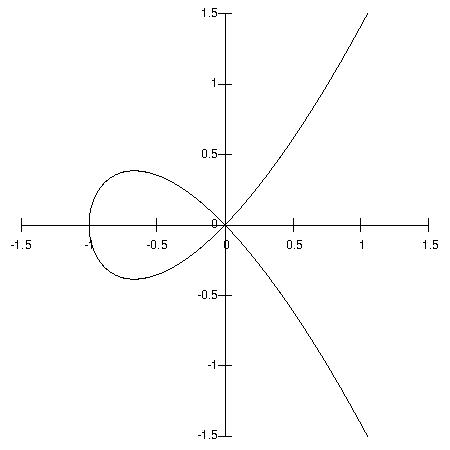
\includegraphics[width=\textwidth]{Algebra2Par29-pic2.pdf}
\end{minipage}
\end{tabular}
\section{Dedekindringe}

\begin{Def}

Ein nullteilerfreier Ring heißt \emp{Dedekindring}\index{Dedekindring}, wenn er noethersch, normal und eindimensional ist.

\begin{nnBsp}
\begin{enumerate}
\item[1)] $\mathbb{Z}$, $k[X]$ ($k$ Körper)

\item[2)] diskrete Bewertungsringe

\item[3)] Hauptidealringe (nullteilerfrei)

\item[4)] der ganze Abschluss $\mathcal{O}_d$ von $\mathbb{Z}$ in $\mathbb{Q}(\sqrt{d})$ wobei $d \in \mathbb{Z}$ quadratfrei.

$\mathcal{O}_d = \begin{cases}
\mathbb{Z}[\sqrt{d}] & d \not\equiv 1 \mod 4\\
\mathbb{Z}[\frac{1+\sqrt{d}}{2}] & d \equiv 1 \mod 4
\end{cases}$

\end{enumerate}
\end{nnBsp}

\end{Def}

Beobachtung: Es gibt Dedekindringe, die nicht faktoriell sind: Beispiel: $\mathbb{Z}[\sqrt(-5)]$.\\
($2 \cdot 3 = (1 + \sqrt{-5}) (1 - \sqrt{-5})$).

\begin{DefBem}
Sei $R$ nullteilerfrei, $K = \textrm{Quot}(R)$
\begin{enumerate}
\item[a)] Ein $R$-Untermodul $I \neq (0)$ von $K$ heißt \emp{gebrochenes Ideal}\index{Ideal!gebrochenes} von $R$, wenn es ein $a \in R \setminus \{0\}$ gibt mit $a \cdot I \subseteq R$. (Beispiel: $n \cdot (\frac{1}{n})$ mit $R = \mathbb{Z}$)

\item[b)] Für gebrochene Ideale $I,J$ von $R$ sei $I \cdot J$ der von allen $a \cdot b$, $a \in I, b \in J$, erzeugte $R$-Untermodul von $K$.

\item[c)] Die gebrochenen Ideale von $R$ bilden mit der Multiplikation aus b) ein kommutatives Monoid mit neutralem Element $R$.

\item[d)] Die Einheiten in diesem Monoid heißen \emp{invertierbare} (gebrochene) Ideale.

d.h. $I$ invertiertbar $\Leftrightarrow$ $\exists I'$ mit $I \cdot I' = R$.

\end{enumerate}
\end{DefBem}

\begin{nnBsp}
\begin{enumerate}
\item[0)] Jedes Ideal in $R$.

\item[1)] Jeder endlich erzeugbare $R$-Untermodul von $K$ ist gebrochenes Ideal.

\textbf{denn:} Seien $x_1 = \frac{a_1}{b_1}, \ldots, x_n = \frac{a_n}{b_n}$ Erzeuger von $M$ ($a_i, b_i \in R$) $\Rightarrow$ für $b = b_1 \cdot \ldots \cdot b_n$ ist $b \cdot M \subseteq R$.

\item[2)] Ist $I$ gebrochenes Ideal, so ist $I^{-1} := \{ x \in K : x \cdot I \subseteq R \}$ ebenfalls gebrochenes Ideal: für jedes $a \in I$ ist $a \cdot I^{-1} \subseteq R$.

$I$ ist invertierbar $\Leftrightarrow$ $I \cdot I^{-1} = R$.

\item[3)] $R = k[X,Y]$, $I = (X,Y)$ $\Rightarrow$ $I^{-1} = R$.

\textbf{denn:} für $a = \frac{f}{g} \in I^{-1}$ muss gelten: $a \cdot X \in R$, $a \cdot Y \in R$.

\item[4)] Jedes Hauptideal $\neq (0)$ ist invertierbar: $(a) \cdot (\frac{1}{a} \cdot R) = R$.
\end{enumerate}
\end{nnBsp}

\begin{Bem}\label{2.41}
Jedes invertierbare Ideal in einem Integritätsbereich ist endlich erzeugbar (als $R$-Modul).

\begin{Bew}
Sei $I$ invertierbar, also $I \cdot I^{-1} = R$, dann gibt es $a_i \in I, b_i \in I^{-1}$ mit $1 = \sum_{i=1}^{n} a_i b_i$

\textbf{Beh:} $a_1, \ldots a_n$ erzeugen $I$.

\textbf{denn:} Sei $a \in I$ $\Rightarrow$ $a = a \cdot 1 = a \cdot \sum_{i=1}^{n} a_i b_i = \sum_{i=1}^{n} a_i \underbrace{(a b_i)}_{\in R}$

\end{Bew}
\end{Bem}

\begin{Satz}[Dedekindringe]\label{Satz13}
Für einen nullteilerfreien Ring $R$ sind äquivalent:

\begin{enumerate}
\item[(i)] $R$ ist Dedekindring oder Körper.

\item[(ii)] $R$ ist noethersch und $R_\mathfrak{p}$ ist diskreter Bewertungsring für jedes Primideal $\mathfrak{p} \neq (0)$ in $R$.

\item[(iii)] Jedes Ideal $I \neq (0)$ in $R$ ist invertierbar.

\item[(iv)] Die gebrochenen Ideal in $R$ bilden eine Gruppe.

\item[(v)] Jedes echte Ideal in $R$ ist Produkt von endlich vielen Primidealen.

\item[(vi)] Jedes echte Ideal besitzt eine eindeutige Darstellung als Produkt von endlich vielen Primidealen.
\end{enumerate}

\end{Satz}

\begin{Bew}

\textbf{Beweisplan:}
\[
\begin{xy}
\xymatrix{
                 & (ii) \ar@{=>}[dr] &                              & (v) \ar@{<=>}[dd] \\
(i) \ar@{=>}[ur] &                   & (iii) \ar@{=>}[dl] \ar@{<=>}[ur] \\
                 & (iv) \ar@{=>}[ul] &                              & (vi) 
}
\end{xy}
\]

\begin{description}
\item[(i) $\Rightarrow$ (ii)]:

Sei $\mathfrak{p} \neq (0)$ Primideal im Dedekindring $R$. $\Rightarrow$ $R_\mathfrak{p}$ noethersch, $\dim R_\mathfrak{p} = \textrm{lat}(\mathfrak{p}) = 1$, da $\dim R = 1$.

$R_\mathfrak{p}$ normal: Sei $a \in K = \textrm{Quot}(R) = \textrm{Quot}(R_\mathfrak{p})$ ganz über $R_\mathfrak{p}$.

Dann gibt es eine Gleichung: $a^n + \sum_{i=0}^{n-1} \frac{b_i}{s_i} a^i = 0$ mit $b_i \in R, s_i \in R \setminus \mathfrak{p}$

$\Rightarrow$ $(s \cdot a)^n + \sum_{i=0}^{n-1} \widetilde{b_i} (s a)^i = 0$ mit $\widetilde{b_i} \in R$, $s := \prod_{i=0}^{n-1} s_i$

$\underset{R \text{ normal}}{\Longrightarrow}$ $s \cdot a \in R$ $\Rightarrow$ $a \underset{s \notin \mathfrak{p}}{=} \frac{s \cdot a}{s} \in R_\mathfrak{p}$

\item[(iii) $\Rightarrow$ (iv)]:

Sei $(0) \neq I \subset K$ gebrochenes Ideal, $a \in R \setminus \{0\}$ mit $a \cdot I \subseteq R$. $\underset{\text{(iii)}}{\Rightarrow}$ $a \cdot I$ invertierbar. $\Rightarrow$ $R = (a \cdot I) \cdot I' = I \cdot (a \cdot I')$ $\Rightarrow$ $I$ ist invertierbar.

\item[(ii) $\Rightarrow$ (iii)]:

Sei $I \neq (0)$ Ideal in $R$. $K = \textrm{Quot}(R)$. $I^{-1} := \{ x \in K : x \cdot I \subseteq R \}$
	
Zu zeigen: $I \cdot I^{-1} = R$.

Annahme: $I \cdot I^{-1} \subsetneqq R$:\\
Dann gibt es ein maximales Ideal $\mathfrak{m}$ von $R$ mit $I \cdot I^{-1} \subseteq \mathfrak{m}$.\\
$\Rightarrow$ $R_\mathfrak{m}$ ist diskreter Bewertungsring.\\
$\Rightarrow$ $I \cdot R_\mathfrak{m}$ ist Hauptideal, d.h. $I \cdot R_\mathfrak{m} = \frac{a}{s} \cdot R_\mathfrak{m}$ für ein $a \in I, s \in R \setminus \mathfrak{m}$

Seien $b_1, \ldots, b_n \in I$ Erzeuger ($R$ ist noethersch). $\Rightarrow$ $\frac{b_i}{1} = \frac{a}{s} \cdot \frac{r_i}{s_i}$ für gewisse $r_i \in R, s_i \in R \setminus \mathfrak{m}$

Sei $t = s \cdot \prod_{i=1}^{n} s_i$. Es gilt: $t \in R \setminus \mathfrak{m}$.

Für jedes $i = 1, \ldots n$ ist $\frac{t}{a} \cdot b_i = r_i \cdot s_i \cdot \ldots \cdot \widehat{s_i} \cdot \ldots \cdot s_n \in R$.

$\Rightarrow$ $\frac{t}{a} \in I^{-1}$ $\Rightarrow$ $t = a \cdot \frac{t}{a} \in I \cdot I^{-1} \subseteq \mathfrak{m}$. Widerspruch.

\item[(iv) $\Rightarrow$ (i)]:

\underline{$R$ noethersch}: Nach \myref{Bemerkung}{2.41} ist jedes invertierbare Ideal endlich erzeugbar.

\underline{$R$ normal}: Sei $x \in K$ ganz über $R$. $\Rightarrow$ $R[x]$ ist endlich erzeugbarer $R$-Modul, also gebrochenes Ideal (Beispiel 1). $\underset{\text{(iv)}}{\Rightarrow}$ $R[x]$ ist invertierbar. 

Da $R[x]$ Ring ist, gilt $R[x] \cdot R[x] = R[x]$. $\underset{R[x]\text{ invertierbar}}{\Longrightarrow}$ $R[x] = R$ (neutrale Element).

$\Rightarrow$ $x \in R$.

\underline{$\dim R \leq 1$}: Sei $\mathfrak{p} \neq (0)$ Primideal in $R$, $\mathfrak{m} \subseteq R$ maximales Ideal mit $\mathfrak{p} \subseteq \mathfrak{m}$.

$\Rightarrow$ $\mathfrak{m}^{-1} \cdot \mathfrak{p} \subseteq \mathfrak{m}^{-1} \mathfrak{m} \underset{\text{(iv)}}{=} R$ und $\mathfrak{m} \cdot (\mathfrak{m}^{-1} \mathfrak{p}) = \mathfrak{p}$.

$\underset{\mathfrak{p}\text{ Primideal}}{\Longrightarrow}$ $\mathfrak{m} = \mathfrak{p}$ oder $\mathfrak{m}^{-1} \mathfrak{p} \subseteq \mathfrak{p}$.

Falls $\mathfrak{m}^{-1} \mathfrak{p} \subseteq \mathfrak{p}$ $\underset{\cdot \mathfrak{p}^{-1}}{\Rightarrow}$ $\mathfrak{m}^{-1} \subseteq R$. Widerspruch (da sonst $\mathfrak{m}^{-1} \cdot \mathfrak{m} \subseteq \mathfrak{m}$)

\item[(iii) $\Rightarrow$ (v)]:

Sei $I \neq (0)$, $I \neq R$ Ideal in $R$.

Setze $I_0 := I$.

Definiere induktiv: $I_n$ für $n \geq 1$:

Ist $I_{n-1} \neq R$, so sei $\mathfrak{m}_{n-1}$ maximales Ideal mit $I_{n-1} \subseteq \mathfrak{m}_{n-1}$ und $I_n := I_{n-1} \mathfrak{m}_{n-1}^{-1} \subseteq R$.

Es ist $I_{n-1} \subseteq I_n$

Wäre $I_n = I_{n-1}$, so wäre $\mathfrak{m}_{n-1}^{-1} = R$. Widerspruch zu $\mathfrak{m}_{n-1}^{-1} \cdot \mathfrak{m}_{n-1} = R$.

Da nach \ref{2.41} $R$ noethersch ist, wird die Kette $I_0 \subsetneqq I_1 \subsetneqq I_2 \subsetneqq \cdots$ stationär.

$\Rightarrow$ $\exists n$ mit $R = I_n = I_{n-1} \mathfrak{m}_{n-1}^{-1} = I_{n-2} \mathfrak{m}_{n-2}^{-1} \mathfrak{m}_{n-1}^{-1} = \cdots = I_0 \cdot \prod_{i=0}^{n-1} \mathfrak{m}_{i}^{-1}$

$\Rightarrow$ $I = I_0 = \prod_{i=0}^{n-1} \mathfrak{m}_i$

\item[(v) $\Rightarrow$ (vi)]:

Sei $\mathfrak{p}_1 \cdots \mathfrak{p}_n = \mathfrak{q}_1 \cdots \mathfrak{q}_m$ mit Primidealen $\mathfrak{p}_i$, $\mathfrak{q}_i$. Zu zeigen: $n=m$ und $\mathfrak{p}_i = \mathfrak{q}_{\sigma(i)}$ für eine Permutation $\sigma \in S_n$:

Induktion über $n$:

$n=1$: $\mathfrak{p} = \mathfrak{p}_1 = \mathfrak{q}_1 \cdots \mathfrak{q}_m$ $\underset{\mathfrak{p}\text{ prim}}{\Rightarrow}$ $\exists\, i_0$ mit $\mathfrak{q}_{i_0} \subseteq \mathfrak{p}$. Umgekehrt ist $\mathfrak{p} \subseteq \mathfrak{q}_i$ für jedes $i$. $\Rightarrow$ $\mathfrak{p} = \mathfrak{q}_{i_0}$

$n>1$: Ohne Einschränkung $\mathfrak{p}_1$ minimal bzgl. $\subseteq$ in $\{ \mathfrak{p}_1, \ldots \mathfrak{p}_n \}$.

Aus $\prod \mathfrak{q}_i \subseteq \prod \mathfrak{p}_j \subseteq \mathfrak{q}_{i_1}$ $\Rightarrow$ $\exists j_0$ mit $\mathfrak{p}_{j_0} \subseteq \mathfrak{q}_{i_0} \subseteq \mathfrak{p}_1$ $\underset{\mathfrak{p}_1\text{ minimal}}{\Rightarrow}$ $\mathfrak{p}_1 = \mathfrak{q}_{i_0}$ $\underset{\text{(iii)}}{\Rightarrow}$ $\mathfrak{p}_2 \cdots \mathfrak{p}_n = \mathfrak{q}_1 \ldots \widehat{\mathfrak{q}_{i_0}} \ldots \mathfrak{q}_m$ $\Rightarrow$ Behauptung aus Induktionsvoraussetzung.

\item[(v) $\Rightarrow$ (iii)]:

Sei $I \neq (0)$, $I = \mathfrak{p}_1 \cdots \mathfrak{p}_r$ mit Primidealen $\mathfrak{p}_i$. Ist jedes $\mathfrak{p}_i$ invertierbar, so ist $I^{-1} = \mathfrak{p}_1^{-1} \ldots \mathfrak{p}_r^{-1}$ und $I \cdot I^{-1} = R$. Also ohne Einschränkung $I = \mathfrak{p}$ Primideal.

Sei $a \in \mathfrak{p} - \{0\}$, $(a) = \mathfrak{q}_1 \ldots \mathfrak{q}_n$ mit Primidealen $\mathfrak{q}_i$ $\Rightarrow$ $\mathfrak{q}_i \subseteq \mathfrak{p}$ für ein $i$.

$\mathfrak{q}_i$ ist invertierbar: $\mathfrak{q}_i^{-1} = \frac{1}{a} \cdot R \cdot \mathfrak{q}_1 \cdots \widehat{\mathfrak{q}_i} \cdots \mathfrak{q}_n$

Es genügt also zu zeigen: $\mathfrak{q}_i = \mathfrak{p}$

\textbf{Beh. 1:} Jedes invertierbare Primideal $\mathfrak{q}$ in $R$ ist maximal.

\textbf{Bew. 1:}
Ist $\mathfrak{q}$ nicht maximal, so sei $x \in R \setminus \mathfrak{q}$ mit $\mathfrak{q} + (x) \neq R$.

\textbf{Beh. 2:} Dann ist $(\mathfrak{q} + (x))^2 = \mathfrak{q} + (x^2)$

Dann ist $\mathfrak{q} \subseteq \mathfrak{q} + (x^2) \underset{\text{Beh. 2}}{=} (\mathfrak{q} + (x))^2 \subseteq \mathfrak{q}^2 + (x)$ $(\ast)$

Weiter ist $\mathfrak{q} \subseteq \mathfrak{q}^2 + \mathfrak{q} \cdot (x)$

\textbf{denn:} Sei $b \in \mathfrak{q}$, schreibe nach $(\ast)$ $b = c + r x$ mit $c = \mathfrak{q}^2, r \in R$, dabei ist $r \in \mathfrak{q}$, da $r \cdot x \in \mathfrak{q}$ und $x \notin \mathfrak{q}$.

$\Rightarrow$ $\mathfrak{q} = \mathfrak{q}^2 + \mathfrak{q} \cdot (x)$ (,,$\supseteq$`` ist trivial)

$\Rightarrow$ $\mathfrak{q} = \mathfrak{q} (\mathfrak{q} + (x)) \underset{\mathfrak{q}\text{ invertierbar}}\Rightarrow R = \mathfrak{q} + (x)$ Widerspruch.

\textbf{Bew. 2:} ,,$\subseteq$`` \checkmark, ,,$\supseteq$``

Schreibe beide Seiten als Produkt von Primidealen.

$\mathfrak{q} + (x) = \mathfrak{p}_1 \cdots \mathfrak{q}_r$, $\mathfrak{q} + (x^2) = \mathfrak{q}_1 \cdots \mathfrak{q}_s$.

In $R / \mathfrak{q}$ ist dann: $(\bar{x}) = \bar{\mathfrak{p}}_1 \cdots \bar{\mathfrak{p}}_r$, $(\bar{x})^2 = \bar{\mathfrak{q}}_1 \cdots \bar{\mathfrak{q}}_s = \bar{\mathfrak{p}}_1^2 \cdots \bar{\mathfrak{q}}_r^2$

$(\bar{x}), (\bar{x}^2)$ invertierbar. $\Rightarrow$ $\bar{\mathfrak{p}_i}, \bar{\mathfrak{q}_j}$ invertierbar.

$\underset{\text{,,(iii) + (v) = (vi)``}}{\Rightarrow}$ $\bar{\mathfrak{q}}_i = \bar{\mathfrak{p}}_{\sigma(i)}^2$ $\Rightarrow$ ohne Einschränkung $\mathfrak{q}_i = \mathfrak{p}_i^2$.

\end{description}
\end{Bew}

\begin{Satz} 
Sie $R$ ein Dedekindring, $K = \Quot(R), \; L/K$ endliche separable
Körpererweiterung.
$S$ der ganze Abschluß von $R$ in $L$.\\
Dann ist $S$ ein Dedekindring.
\end{Satz}

\begin{Bew} 
\underline{$\dim S=1:$} Folgt aus \hyperref[Satz10]{Satz~\ref*{Satz10}\ref*{Satz10c}}

\underline{$S$ normal:}\\
Sei $x\in L$ ganz über $S$, also $x^n+\sum_{i=1}^{n-1}a_i x^i = 0$ mit $a_i \in S$.
Sei $S'$ der von $R$ und $a_1,\dots,a_{n-1}$ erzeugte Unterring von $S$.
$S'$ ist endlich erzeugbarer $R$-Modul, da die $a_i$ ganz über $R$ sind.
$S[X]$ ist endlich erzeugter $S'$-Modul und damit endlich erzeugbarer $R$-Modul $\Rightarrow x$ ist ganz über $R \Rightarrow x \in S$.

\underline{$S$ noethersch:}\\
\textbf{Beh. 1:} Es gibt ein primitives Element $\alpha$ von $L/K$ mit $\alpha \in S$.\\
\textbf{Bew. 1:} Sei $\tilde{\alpha} \in L$ primitives Element, also $1, \tilde{\alpha}, \tilde{\alpha}^2, \dots, \tilde{\alpha}^{n-1}$ ist $K$-Basis von $L \; (n \defeqr [L:K])$.
Sei $\tilde{\alpha} = \sum_{i=0}^{n-1} c_i \tilde{\alpha}^i$ für gewisse $c_i \in K, \; i = 0, \dots, n-1$.
Schreibe $c_i = \frac{a_i}{b_i}$ mit $a_i, b_i \in R, \; b \defeqr \prod_{i=0}^{n-1} b_i$.
Setze $\alpha \defeqr b \cdot \tilde{\alpha} \Rightarrow \alpha^n = b^n \cdot
\sum_{i=0}^{n-1} c_i \tilde{\alpha}^i = \sum_{i=0}^{n-1} \underset{\in
R}{\underbrace{c_i b^{n-i}}}\alpha^i \Rightarrow \alpha \in S$

$1, \alpha, \alpha^2, \dots, \alpha^{n-1}$ linear unabhängig:\\
Sei $\sum_{i=0}^{n-1} \lambda_i \alpha^i = 0 \Rightarrow \sum \lambda_i b^i \tilde{\alpha}^i = 0 \Rightarrow \lambda_i b^i = 0 \; \forall i$

Sei nun $\bar{K}$ ein algebraischer Abschluss von K.
Seien $\sigma_1, \dots, \sigma_n$ die verschiedenen Einbettungen von $L$ in
$\bar{K}$, also die Elemente von $\Hom(L,\bar{K})$.\\
$d \defeqr d(\alpha) \defeqr (\det(\sigma_i(\alpha^{j-1})_{i,j=1, \dots, n}))^2$
heißt die Diskriminante von $L/K$ (bzgl. $\alpha$).

\textbf{Beh. 2:}
\vspace{-1.5ex}
\begin{enumerate} 
  \item $d \not= 0$
  \item $S$ ist in dem von $\frac{1}{d}, \frac{\alpha}{d}, \dots,
  \frac{\alpha^{n-1}}{d}$ erzeugten $R$-Untermodul von $L$ enthalten.
\end{enumerate}
Dann ist $S$ als Untermodul eines endlich erzeugbaren $R$-Modul selbst endlich
erzeugbar und damit noethersch (weil $R$ noethersch ist).

\textbf{Bew. 2:}
\begin{enumerate}
\item $d = \det
  \begin{pmatrix}
    1 & 1 & \dots & 1 \\
    \sigma_1(\alpha) & \sigma_2(\alpha) & \dots & \sigma_n(\alpha) \\
    \sigma_1(\alpha)^2 & \sigma_2(\alpha)^2 & \dots & \sigma_n(\alpha)^2 \\
    \vdots & \vdots & \ddots & \vdots \\
    \sigma_1(\alpha)^{n-1} & \sigma_2(\alpha)^{n-1} & \dots & \sigma_n(\alpha)^{n-1}
  \end{pmatrix}
  \overset{\text{Vandermonde}}{=} \displaystyle\prod_{i \not= j}
  (\sigma_i(\alpha) - \sigma_j(\alpha)) \not= 0$

\item Für $x \in L$ sei $\text{Spur}(x) \defeqr \sum_{i=1}^n \sigma_i(x) \in \bar{K}$

  $\text{Spur}(x) \in K:$ Für $\sigma \in \Aut_K(\bar{K})$ ist $\sigma \circ \sigma_i \in \Hom_K(L,\bar{K})$

  $\sigma(\text{Spur}(x)) = \sum_{i=1}^n (\sigma \circ \sigma_i)(x) = \text{Spur}(x) \in \bar{K}^{\Aut_K(\bar{K})} = K$.

  Sei $x \in S, \; x = \sum_{j=1}^n c_j \alpha^j$ mit $c_j \in K$.
\end{enumerate}

\textbf{Beh. 3:} $c = \begin{pmatrix} c_1\\ \vdots\\ c_n \end{pmatrix}$ ist
Lösung eines LGS $A \cdot c = b$ mit $b \in R^n$ und $A \in R^{n \times n}$
mit $\det A = d$.\\
Nach der Cramerschen Regel ist dann $c_i = \frac{\det A_i}{\det A}$ wobei
$A_i$ aus $A$ dadurch entsteht, dass die $i$-te Zeile durch $b$ ersetzt wird.
$\Rightarrow$ $c_i \in \frac{1}{d}R$ $\Rightarrow$ $x$ liegt in 
dem von $\frac{1}{d}, \frac{\alpha}{d}, \dots, \frac{\alpha^{n-1}}{d}$ erzeugten $R$-Modul.

\textbf{Bew. 3:} Für $i=1, \dots, n$ ist $\text{Spur}(\alpha^{i-1} x) = \sum_{j=1}^n \text{Spur}((\alpha^{i-1}\alpha^{j-1})c_j) \in K \quad (*)$ ganz über $R$\\
$\Rightarrow$ $\text{Spur}(\alpha^{i-1}x) \in R \Rightarrow A \defeqr (\text{Spur}(\alpha^{i-1} \alpha^{j-1})_{i,j = 1, \dots, n}) \in R^{n \times n}$

$b \defeqr
\begin{pmatrix}
  \text{Spur}(x) \\
  \text{Spur}(\alpha x) \\
  \vdots \\
  \text{Spur}(\alpha^{n-1}x)
\end{pmatrix} \in R^n$ $(*)$ heißt $A \cdot c = b$.

Noch zu zeigen: $\det A = d$.\\
Nach Definition ist $d = (\det B)^2$ mit $B = (\sigma_i(\alpha^{j-1})_{i,j})$\\
$\Rightarrow$ $B^T \cdot B = (\beta_{ij})$ mit $\beta_{ij} = \sum_{k=1}^n \sigma(\alpha^{i-1}) \sigma_k(\alpha^{j-1}) = \text{Spur}(\alpha^{i-1} \alpha^{j-1})$\\
$\Rightarrow$ $B^T \cdot B = A$ $\Rightarrow$ $\det A = (\det B)^2 = d$
\end{Bew}

\begin{nnBsp}
$K=\mathbb{Q}$, $L=\mathbb{Q}(\sqrt{D})$, $D$ quadratfrei, $R=\mathbb{Z}$.

Was ist $d$? $\alpha = \sqrt{D}$, $\sigma_1=\textrm{id}$, $\sigma_2(a+b\sqrt{D})=a-b\sqrt{D}$

$B=\left(\begin{array}{cc}1&1\\\sqrt{D}&-\sqrt{D}\end{array}\right)$

$d=(\textrm{det}\ B)^2=(-2\sqrt{D})^2=4D$

\end{nnBsp}
\section{Primärzerlegung}

\begin{nnBsp}
$R = k[X,Y]$. $I = (X^2, Y)$ hat keine Darstellung als Produkt von Primidealen.

\textbf{denn}: Wäre $I = \mathfrak{p}_1^{\nu_1} \cdots \mathfrak{p}_r^{\nu_r}$ mit paarweise verschiedenen Primidealen $\mathfrak{p}_i$, so wäre $\sqrt{I} = \mathfrak{p}_1 \cdots \mathfrak{p}_r = (X,Y) = \mathfrak{m}$. also $r = 1$, $\mathfrak{p}_1 = \mathfrak{m}$. Aber: $\mathfrak{m} \supsetneqq I \supsetneqq \mathfrak{m}^2$.

\end{nnBsp}

\begin{DefBem}
Sei $R$ Ring, $\mathfrak{q} \subseteq R$ echtes Ideal.

\begin{enumerate}
\item[a)] $\mathfrak{q}$ heißt \emp{Primärideal}\index{Primärideal}, wenn für alle $a,b \in R$ mit $a \cdot b \in \mathfrak{q}$ und $a \notin \mathfrak{q}$ gilt: es gibt ein $n \geq 1$ mit $b^n \in \mathfrak{q}$.

\item[b)] Ist $\mathfrak{q}$ Primärideal, so ist $\mathfrak{p} = \sqrt{\mathfrak{q}}$ Primideal. $\mathfrak{p}$ heißt zu $\mathfrak{q}$ \emp{assoziiertes}\index{Primideal!assoziiertes} Primideal.

\begin{Bew}
Seien $a, b \in R$ mit $a \cdot b \in \sqrt{\mathfrak{q}}$ $\Rightarrow$ $a^n b^n \in \mathfrak{q}$ für ein $n \geq 1$.

Ist $a \notin \sqrt{\mathfrak{q}}$, so ist $a^n \notin \mathfrak{q}$ $\underset{\text{Def.}}{\Rightarrow}$ $(b^n)^m \in \mathfrak{q}$ $\Rightarrow$ $b \in \sqrt{\mathfrak{q}}$
\end{Bew}

\item[c)] $\mathfrak{q}$ Primärideal $\Leftrightarrow$ jeder Nullteiler in $R / \mathfrak{q}$ ist nilpotent.

\end{enumerate}
\end{DefBem}

\begin{nnBsp}
\begin{enumerate}
\item[1)] Ist $p \in R$ ein Primelement, so ist $(p^n) = (p)^n$ Primärideal für jedes $n \geq 1$.

\textbf{denn}: Seien $a, b \in R$ mit $a \cdot b \in (p^n)$ und $a \notin (p^n)$ Ist $b \in (p)$, so ist $b^n \in (p^n)$.

Anderenfalls ist $a \in (p)$. Dann gibt es $1 \leq d < n$ mit $a \in (p^d) \setminus (p^{d+1})$ $\Rightarrow$ $a = p^d \cdot u$ mit $u \in R \setminus (p)$. Dann ist $u \cdot b \notin (p)$ $\Rightarrow$ $a \cdot b = p^d \cdot u \cdot b \notin (p^{d+1})$ Widerspruch.

\item[2)] Ist $R$ Dedekindring, so sind die Primärideale genau die Potenzen von Primidealen.

\textbf{denn}: Ist $\mathfrak{q}$ Primärideal, $\mathfrak{q} = \mathfrak{p}_1^{\nu_1} \cdots \mathfrak{p}_r^{\nu_r}$ die Zerlegung von $\mathfrak{q}$ in Primidealen.\\
$\Rightarrow$ $\sqrt{\mathfrak{q}} = \mathfrak{p}_1 \cdots \mathfrak{p}_r$ $\underset{\sqrt{\mathfrak{q}}\text{ ist prim}}\Rightarrow$ $r=1$.

Sei umgekehrt $\mathfrak{q} = \mathfrak{p}^n$ für ein Primideal $\mathfrak{p}$, $n \geq 1$. Seien $a, b \in R$, $a \cdot b \in \mathfrak{p}^n$, $a \notin \mathfrak{p}^n$. Nach \myref{Satz}{Satz13} ist $R_\mathfrak{p}$ Hauptidealring. D.h. $\mathfrak{p} R_\mathfrak{p}$ wird erzeugt von einem $\frac{p}{s}$, wobei $p \in \mathfrak{p}, s \in R \setminus \mathfrak{p}$ $\underset{\text{Bsp 1}}\Rightarrow$ $\mathfrak{p}^n R_\mathfrak{p} = (\mathfrak{p} R_\mathfrak{p})^n$ ist Primideal.

Ist $a \in \mathfrak{p}^n R_\mathfrak{p}$, so ist $a = \frac{p^n}{s^n} \cdot \frac{u}{t}$ mit $u \in R, t \in R \setminus \mathfrak{p}$ $\Rightarrow$ $t \cdot s^n \cdot a \in \mathfrak{p}^n$ $\Rightarrow$ $a \in \mathfrak{p}^n$. Widerspruch.

Anderenfalls ist $b^m \in \mathfrak{p}^n R_\mathfrak{p}$ für ein $m$ und damit $b \in \mathfrak{p}$ und $b^n \in \mathfrak{p}^n$.

\end{enumerate}
\end{nnBsp}

\begin{Bem}
Sind $I_1, \ldots I_r$ $\mathfrak{p}$-primär (d.h. $I_i$ primär und $\sqrt{I_i} = \mathfrak{p}$), so ist auch $I := \displaystyle\bigcap_{i=1}^{r} I_i$ $\mathfrak{p}$-primär.

\begin{Bew}
Seien $a,b \in R$ mit $a \cdot b \in I$, $a \notin I$. Dann gibt es $i$ mit $a \notin I_i$ $\Rightarrow$ $b^{n_i} \in I_i$ für ein $n_i \geq 1$ $\Rightarrow$ $b \in \sqrt{I_i} = \mathfrak{p}$ $\Rightarrow$ Für $j = 1, \ldots r$ gibt es $n_j \geq 1$ mit $b^{n_j} \in I_j$ $\Rightarrow$ $b^n \in I$ für $n = \max_{j=1}^{n} n_j$.

\end{Bew}
\end{Bem}

\begin{Def}
Sei $I$ Ideal in $R$.

\begin{enumerate}
\item[a)] Eine Darstellung $I = \mathfrak{q}_1 \cap \cdots \cap \mathfrak{q}_r$ heißt \emp{Primärzerlegung}\index{Primärzerlegung} von $I$, wenn alle $\mathfrak{q}_i$ primär sind.

\item[b)] Eine Primärzerlegung heißt \emp{reduziert}\index{Primärzerlegung!reduziert}, wenn $\sqrt{\mathfrak{q}_i} \neq \sqrt{\mathfrak{q}_j}$ für $i \neq j$ und kein $\mathfrak{q}_i$ weggelassen werden kann.

\item[c)] Besitzt $\mathfrak{q}$ eine Primärzerlegung, so auch eine reduzierte.
\end{enumerate}
\end{Def}

\begin{Satz}[Reduzierte Primärzerlegung]
Sei $R$ noetherscher Ring.

Dann hat jedes echte Ideal in $R$ eine reduzierte Primärzerlegung. Die assoziierten Primideale sind eindeutig. Die Primärideale, deren assoziierten Primideale minimal unter den in der Zerlegung vorkommenden sind, sind ebenfalls eindeutig.

\begin{Bew}
Sei $\mathcal{B} = \{ I \subset R \text{ Ideal} : I \text{ besitzt keine Primärzerlegung} \}$. Ist $\mathcal{B} \neq \emptyset$, so besitzt $\mathcal{B}$ ein maximales Element $I_0$. Da $I_0$ nicht primär ist, gibt es $a,b \in R$ mit $a \cdot b \in I_0$ und $a \notin I_0$ und $b^n \notin I_0$ für alle $n \geq 1$.

\textbf{Ziel}: Konstruiere Ideale $I$ und $J$ mit $I_0 = I \cap J$ und $I \neq I_0 \neq J$. Dann haben $I$ und $J$ Primärzerlegungen, also $I_0$ auch. Widerspruch!

Für $n \geq 1$ sei $I_n := \{ c \in R : c \cdot b^n \in I_0 \}$. $I_n$ ist Ideal mit $I_0 \subseteq I_n \subseteq I_{n+1}$. Da $R$ noethersch ist, gibt es $k \in \mathbb{N}$ mit $I_n = I_k$ für alle $n \geq k$. Setze $I := I_n$. Beachte $a \in I_1 \setminus I_0 \subseteq I \setminus I_0$.

Sei $J := I_0 + (b^k) \supsetneqq I_0$, da $b^k \notin I_0$.

\textbf{Beh}: $I \cap J = I_0$

\textbf{denn}: ,,$\supseteq$`` \checkmark ,,$\subseteq$`` Sei $y \in I \cap J$, also $y = x + b^k \cdot r$ (für ein $x \in I_0, r \in R$) und $y \cdot b^k \in I_0$ $\Rightarrow$ $y \cdot b^k = b^{2k} \cdot r + x \cdot b^k$ $\Rightarrow$ $r \cdot b^{2k} = y b^k \cdot x b^k$ $\Rightarrow$ $r \in I_{2k} = I_k$ $\Rightarrow$ $r \cdot b^k \in I_0$ $\Rightarrow$ $y \in I_0$.

\end{Bew}
\end{Satz}

\appendix

\def\indexspace{\par\medskip}
\printindex[default][\phantomsection\addcontentsline{toc}{chapter}{Vokabeln}\vspace{-1.2em}]

\end{document}
